%% LyX 2.2.3 created this file.  For more info, see http://www.lyx.org/.
%% Do not edit unless you really know what you are doing.
\RequirePackage{fix-cm}
\documentclass[12pt,twoside,english]{article}
\usepackage[latin9]{inputenc}
\usepackage[a4paper]{geometry}
\geometry{verbose,tmargin=24.75mm,bmargin=48.5mm,lmargin=23.25mm,rmargin=31.5mm}
\pagestyle{headings}
\usepackage{babel}
\usepackage{array}
\usepackage{rotating}
\usepackage{varioref}
\usepackage{float}
\usepackage{mathtools}
\usepackage{multirow}
\usepackage{amsmath}
\usepackage{amssymb}
\usepackage{makeidx}
\makeindex
\usepackage{graphicx}
\usepackage{setspace}
\usepackage[numbers]{natbib}
\onehalfspacing
\usepackage[unicode=true]
 {hyperref}

\makeatletter

%%%%%%%%%%%%%%%%%%%%%%%%%%%%%% LyX specific LaTeX commands.
%% Because html converters don't know tabularnewline
\providecommand{\tabularnewline}{\\}
\floatstyle{ruled}
\newfloat{algorithm}{tbp}{loa}
\providecommand{\algorithmname}{Algorithm}
\floatname{algorithm}{\protect\algorithmname}

%%%%%%%%%%%%%%%%%%%%%%%%%%%%%% User specified LaTeX commands.
% how to get rid of overfull hboxes:
\tolerance=1600
%\sloppy
%\setlength\emergencystretch{2em}

% \bot or \perp sign with two parallel vertical lines, for independency between random variables
\newcommand{\indep}{\rotatebox[origin=c]{90}{$\models$}}

\makeatother

\begin{document}

\title{\vspace{-1.4cm}
\textbf{Semi-supervised Classification}\\
\textbf{of Breast Cancer Expression Profiles}\\
\textbf{Using Neural Networks}}

\date{~}

\maketitle
\thispagestyle{empty}

\vspace{-1.5cm}
\begin{center}

\includegraphics[width=0.25\paperwidth]{images/sigillum}
\par\end{center}

\vspace{0.9cm}
\begin{spacing}{1.6}
\begin{center}
\textsc{\large{}Dissertation zur Erlangung des Doktorgrades}\\
\textsc{\large{}der Naturwissenschaften (Dr. rer. nat.)}\\
\textsc{\large{}der Fakult�t f�r Biologie und Vorklinische Medizin}\\
\vspace{0.3cm}
\textsc{\large{}der Universit�t Regensburg}
\par\end{center}{\large \par}
\end{spacing}

\vspace{0.8cm}
\begin{center}
{\large{}vorgelegt von}
\par\end{center}{\large \par}

\begin{center}
\textbf{\textsc{\Large{}Anton G. Moll}}
\par\end{center}{\Large \par}

\begin{center}
{\large{}aus Starnberg}
\par\end{center}{\large \par}

\vspace{0.3cm}
\begin{center}
{\large{}im Jahr 2017}
\par\end{center}{\large \par}

\clearpage{}

\thispagestyle{empty}

\cleardoublepage{}

\thispagestyle{empty}\vspace*{2cm}

\noindent{Promotionsgesuch eingereicht am: 22. September 2017}\vspace{1cm}

\noindent{Die Arbeit wurde angeleitet von:}
\begin{enumerate}
\item Prof. Dr. Rainer Spang
\item Prof. Dr. Rainer Merkl
\end{enumerate}
\vspace*{12cm}

Unterschrift\hfill{}Regensburg, den 22. September 2017

\clearpage{}

\section*{Acknowledgements}

This work was carried out in the department for \emph{Statistical
Bioinformatics} of the Institute of Functional Genomics at the University
of Regensburg. I am grateful to Rainer Spang for the opportunity to
work in his group.

I would like to thank my two supervisors \emph{Rainer Spang }and \emph{Rainer
Merkl }for their constant advice. Especially I would like to thank
my advisor \emph{Claudio Lottaz }for the scientific discussions and
input he gave me during the past years.

I thank all past and present colleagues for the pleasant working athmosphere
and fruitful scientific and non-scientific discussions. In particular
I would like to thank my past and present office mates \emph{Christian
H.,} \emph{Farhad}, \emph{Frank}, \emph{Franziska}, \emph{Julia},
\emph{Nicholas}, \emph{Martin, }and \emph{Qian.}

I would also like to thank my family for their support. Special thanks
go to my sister \emph{Susanne} for proofreading and commenting on
a draft of this thesis.


\cleardoublepage{}\tableofcontents{}

\cleardoublepage{}


\section{Summary}

In classification tasks of biological data, there are usually fewer
labeled than unlabeled samples because labeling samples is costly
or time-consuming. In addition, labeled data sets can be re-used in
different contexts as additional unlabeled data sets. For example,
when searching the Gene Expression Omnibus (GEO) repository for microarray
data sets of drug sensitivity and resistance experiments, the largest
one has 2,522 samples, but the median has only 12 samples.

In machine learning in general, utilizing unlabeled data in classification
tasks is called semi-supervised learning. Artificial neural networks
can be used to pre-train on unlabeled data before fine-tuning via
back-propagation with labeled data. Such artificial neural networks
enabling deep learning have gained attention since around 2010, since
when they have been among the best-performing algorithms in visual
object recognition.

We measured accuracies in the task of classifying tissue taken from
breast cancer patients at reductive surgery as chemotherapy-resistant
or -sensitive. Different data sets were constructed by subsampling
from GEO data set GSE25055 and GSE25065. Using these data sets, we
compared classification accuracy of the neural networks autoencoder,
Restricted Boltzmann Machine, Deep Belief Network (DBN) and support
vector machine (SVM), and Transductive SVM (TSVM). Training was done
both in supervised and semi-supervised mode. For the neural networks,
we tried several different network architectures. 

Smoothing the validation set accuracies obtained during training iterations
to alleviate low sample numbers helped in model selection of the best
classifier. We also investigated the effect of different normalization
procedures on the classification accuracy. The data were normalized
with either RMA or MAS5, followed by either no batch-effect correction
or Combat batch-effect correction. Only MAS5 profited from added Combat
batch-effect correction, but normalization with RMA alone yielded
the best classification accuracy.

We were particularly interested whether classification accuracies
improve when adding unlabeled samples in semi-supervised learning.
Overall, neural networks and support vector machines performed similar.
We found a slight improvement of classification accuracy when the
number of unlabeled samples presented to DBN and TSVM was increased
to the maximal number of samples in our data sets. However, this effect
was only observed when the learning algorithms were presented the
expression values of all 22,283 genes, not just the 500 most variable
genes.


\cleardoublepage{}

\part{Introduction}


\section{Personalized Medicine}

A medium-term goal of medicine is ``personalized medicine\index{personalized medicine}'',
whose goal is to provide custom-tailored health care on an individual
basis. For example, a standard treatment for breast cancer is chemotherapy,
but not all patients profit from this treatment. The event that a
patient has no sign of breast cancer after reductive surgery followed
by chemotherapy is called \emph{pathologic complete response}\index{pathologic complete response}\index{pCR},
and the opposite event that the patient still has cancerous tissue
after this procedure is called \emph{residual disease}\index{residual disease}\index{RD}.

Suppose there were a predictor that could tell the physicist how likely
a patient is to benefit from chemotherapy. If the prediction for a
certain patient was such that complete response to chemotherapy was
unlikely, chemotherapy could be replaced by another therapy.

The goal of this work is to contribute to such a predictor. The input
to the predictor is the molecular expression data, i.e. measures of
the number of RNA copies of specific genes present in the cancer tissue.
These gene expression measurements are ususally measured using microarrays
or next generation sequencing. An artificial neural network then processes
this data. The prediction is output by the network in the form of
a number between 0 and 1. Here, 0 means the patient is predicted with
absolute certainty to have residual disease, 1 means the patient is
predicted with absolute certainty to have pathologic complete response,
and a number in-between is interpreted as the probability for pathologic
complete response.

The study of neural networks in biology prompted the development of
artificial neural networks as models of biological neural networks.
After an introduction to biological and artificial neural networks
we will give an overview of the relevant topics of machine learning
and then introduce the own work done in this manuscript.

\section{Biological and Artificial Neural Networks}

Artificial neural networks\index{artificial neural networks} are
mathematical constructs, designed to imitate the signal processing
capabilities of real neurons, found in nearly all animals. Neurons
can be connected to form complex neural networks. Like their biological
counterparts, artificial neural networks consist of simpler building
blocks, the neurons.

\subsection{Neurons As Basic Signal Processing Units}

The biological neurons are defined (according to the neuron doctrine
\cite{BullockDouglas2005}) as the smallest units whose state change
may be called signal processing, so they are the basic signal processing
units. They have multiple inputs at dendrites, and multiple outputs
at axon terminals \cite{ByrneDafny1997}. Figure \ref{fig:Schematic-image-of-biological-neurons}
gives a schematic overview of these elements.

\begin{figure}
\begin{centering}
\includegraphics[width=0.8\columnwidth]{images/neurons}
\par\end{centering}
\caption[Schematic image of three biological neurons.]{\label{fig:Schematic-image-of-biological-neurons}Schematic image
of three biological neurons. A: neuron body B: nucleus C: dendrite
D: synapse E: axon projecting from a distant neuron.}
\end{figure}

In most real neurons, the signal transmission and processing is facilitated
by alternating small electric (action) potentials (along the axons)
and chemical transmissions (at chemical synapses between axon and
dendrite). The electric potential is transmitted along the dendrites
of a neuron, and flows to the axon of the neuron, where it can lead
to the release of neurotransmitters stored in the axon terminals into
the synaptic cleft. The released neurotransmitters are detected by
receptors and cause ion channels in the adjacent dendrites of other
neurons to open, which changes their membrane potential. See figure
\ref{fig:Schema-of-chemical-synapse} for a depiction of axon, synaptic
cleft, and dendrite.

\begin{figure}[t]
\begin{centering}
\includegraphics[width=0.8\columnwidth]{images/synapse}
\par\end{centering}
\caption[Schema of a chemical synapse.]{\label{fig:Schema-of-chemical-synapse}Schema of a chemical synapse.
The signal is transmitted from the axon terminal (left) to the dendrite
(right). Grey: membranes of neurons. Green and blue: ion transporters
maintain intracellular ion concentrations. Red: neurotransmitter is
stored inside the cell in vesicles and emitted into the synaptic cleft
upon an electric potential arriving at the axon terminal. Purple:
receptors signal to the inside of the cell the absence or presence
of neurotransmitter on the outside of the cell.}
\end{figure}

\subsubsection{Action Potentials, Their Propagation, and Chemical Synapses }

The action potentials are realized by cells in the form of different
ion concentrations inside and outside the cell. These ion gradients
are maintained in the resting state by the $Na^{+}/K^{+}$-ATPases
that pump 3 $Na^{+}$ ions out of and 2 $K^{+}$ ions into the cell
for every ATP molecule \cite{LodishZipursky2000}. Because ions are
charged, there is an electric potential between the outside and inside
of the cell. The resting potential is between $-80$mV and $-40$mV,
depending on the type of neuron. The electric potential becoming more
positive is called depolarization, and the opposite hyperpolarization.

The propagation of the action potentials along dendrites is realized
by the opening and closing of ion channels. Once depolarization of
an adjacent region of a neuron causes the electric potential between
the inside and outside of a $Na^{+}$ ion channel to reach a critical
value, the ion channel opens, causing further depolarization in adjacent
regions of the neuron. This positive feedback loop continues until
all $Na^{+}$ channels are open. At the peak of depolarization, $K^{+}$
ion channels open, causing hyperpolarization, and the potential returns
to the resting  potential. This makes the action potential travel
along the neuron. Once it has reached an axon terminal, it causes
neurotransmitter release.

Neurotransmitters binding to receptors present on the outside of
the neuron's membrane cause ion channels to open, and the ions flow
into or out of the cell to achieve equilibrium of ion concentration.
The type of ion channel being opened upon binding of a neurotransmitter
can cause either depolarization or hyperpolarization of the dendrite,
depending on the charge of the ion, and whether the resting concentration
of the ion is higher intracellular or extracellular. If a critical
threshold of depolarization is reached, the $Na^{+}$ ion channels
will open, and an action potential ``spike'' is generated as described
above.

\subsubsection{Encoding of Information in Action Potentials}

The presence of a critical threshold suggests that it is not the ``analog''
electric potential, but the ``digital'' spike that carries the information
from one neuron to the next. For example, the strength muscles are
innervated with, is encoded in the number of action potentials per
time delivered by the muscle neuron to the muscle fiber. However,
some neurons involved in perception directly transmit information
in the fluctuations of neurotransmitter released. This analog mode
of transmission allows more information to be transmitted per time.
Sub\-threshold emission of neurotransmitter also seems to modulate
subsequent action potentials, allowing for a mixture of analog and
digital information transmission \cite{DebanneRama2013}. 

Examples for neural networks that have been partly decoded are the
eye (visual system) and the nose (olfactory system).

\subsection{Examples of Biological Neural Networks}

\subsubsection{The Eye, a Visual System}

In the eye, specialized cells called rods and cones detect light\cite{Biochemistry2002,Kolb2003}.
Rods are more sensitive to dim light, while the three types of cones
react to bright light only but can differentiate between colors. Both
rods and cones release the neurotransmitter glutamate continuously
into the synaptic cleft, but when hit by light, suspend this emission
for the duration of the light. This is implemented by the cell by
a long pathway.

Specifically, light elicits a transformation of cis-rhodopsin to trans-rhodopsin,
which presents on its surface a G protein binding site. The G protein
transducin binds to the activated rhodopsin, and in this process GDP
acquires a phosphate group to form GTP. The $\alpha$-subunit of transducin
activates a cGMP phosphodiesterase, which in turn hydrolyzes cGMP
to GMP. The reduction in the concentration of cGMP causes cGMP-gated
ion channels to close. This in turn hyperpolarizes the photosensitive
cell, causing glutamate to be released into the synaptic cleft at
a slower rate. This long pathway between cis-rhodopsin and glutamate
release inhibition facilitates an amplification of the signal at every
step, which allows rod cells to signal a spike in response to it being
hit by a single photon.

The area that elicits a response in the cell upon being illuminated
is called the \emph{receptive field}\index{receptive field}, and
is just as large as the top of the photoreceptor for rods and cones.
The released glutamate binds to receptors present on the outside of
bipolar cells, and, depending on the type of bipolar cell, cause either
an action potential to be generated when the photoreceptor is lit
and the surrounding area is dark (\emph{ON }bipolar cell), or when
the photoreceptor is dark against a bright background (\emph{OFF }bipolar
cell). Another type of cell, the horizontal cell integrates signals
from surrounding cone cells, and feed their signal back to the cones,
or directly to bipolar cells. This enhances contrast. The signal from
several bipolar cells is fed into a ganglion cell, which therefore
has a larger receptive field than its connected bipolar cells. ON
bipolar cells only excite ON ganglion cells, and OFF bipolar cells
excite only OFF ganglion cells. Finally, in primates, there are more
than a million nerve fibers from ganglion cells to the visual cortex
of the brain. Altogether, the basic cell types are, depending on the
species, 1 to 4 types of horizontal cells, 11 types of bipolar cells,
22 to 30 types of amacrine cells, and 20 types of ganglion cells.
Among those cell types' known functions are integration of a large
number of rods to provide sight in little light, brightness-dependent
size regulation of the receptive field of amacrine cells, and an additional
photoreceptor distinct from rods and cones\cite{Kolb2003}.


\subsubsection{Odor Sensing in the Olfactory System}

The olfactory system of mammals and insects contains neurons that
detect odor molecules, called glomeruli\cite{ZhangSharpee2016}. In
humans, there are about $500$ different types of glomeruli {[}1{]},
but it is hypothesized that a human can perceive around $10,000$
different odors. Each ``atomic'' odor consisting of a few ($<100$)
molecular species excites one or more glomeruli, and the compression
requires each glomerulus to signal the presence of one or more than
one odor. The excitation pattern of multiple glomeruli must be resolved
in the olfactory neuronal system so that a low-dimensional vector
of ($\approx500$) glomeruli activations is decompressed to a high-dimensional
representation of ($\approx10,000$) odors in the brain.

Each glomerulus is connected to one or more Kenyon Cells in insects.
It is assumed that the activation of a Kenyon cell signals to the
insect nervous system the presence of one specific odor. (In the mammalian
brain, a single odor is represented by neurons in the olfactory cortex.)
Experiments show that the circuit connecting glomeruli to Kenyon cells
is feed-forward\index{feed-forward neural network} only, i.e. without
recurrent connections (loops). The structure of a feed-forward compressed
sensing circuitry is of interest, because standard compressed sensing
circuits are recurrent dynamic systems that converge to one of their
attractor states. In addition to quick decoding of odors, experimental
evidence shows that the biological compressed sensing circuitry is
robust to noise, i.e. to spurious neuronal spikes in glomeruli, or
noise due to experimental inhibition\footnote{Also experimental modifications of glomeruli have been made so that
half of all glomeruli always express only one type of receptor.} of glomeruli.

The theoretical work of \cite{ZhangSharpee2016} proposed that a feed-forward
architecture could facilitate odor decoding simply by implementing
a logical AND. They suggest that in the neuronal AND-circuit a specific
odor's Kenyon cell is activated when at least (for example) $80\%$
of the glomeruli with receptors to this odor are active. On a cellular
level, this could be realized by connecting the glomeruli associated
with an odor with the odor's Kenyon cell, and a threshold at the Kenyon
cell's input.

A prediction of \cite{ZhangSharpee2016} is that the number of glomeruli
activated by a single odor should be close to the number of glomeruli
that are connected to a Kenyon cell. They postulated further that
the validity of their feed-forward model can be tested by measuring
the odor sparseness\footnote{Odor sparseness is the average number of different molecular species
in an odor.} in the environment of an animal species and comparing it to its average
number of connections from glomeruli to Kenyon cells.

For example, in \emph{Drosophila}, about $9\%$ of the glomeruli are
excited by an odorant, and the connectivity rate between glomeruli
and Kenyon Cells is between $6.5\%$ and $12.5\%$. In the locust,
a projection neuron (the equivalent to a glomerulus) is activated
by half of the odorants and the connectivity rate is about $50\%$.
This is in agreement with the proposed model.

The model also predicts that species with sparse connectivity have
better odor perception of complex odor mixtures. On the other hand,
species with dense connectivity should have better olfactory performance
in detecting simple odor mixtures.

\subsection{Artificial Neurons as Simple Models of Biological Neurons\label{subsec:Artificial-Neurons-as-Simple-Models-of-Biological-Neurons}}

The machinery facilitating propagation and transmission of information
in and between biological neurons is highly simplified in artificial
neurons\index{artificial neuron signal processing}. Signal processing
of a real neuron is modelled in an artificial neuron as a mathematical
function that has multiple input variables, computes a value according
to the function formula and its parameters and outputs its computed
value to multiple neurons, which use it as an input variable. Herein,
the processes of neurotransmitter release, de- and hyperpolarization,
and propagation of the action potential are abstracted away into discrete
time steps.

Each artificial neuron's function is evaluated once per time step.
Often, the \emph{sigmoid}\index{sigmoid function}\emph{ }function
is used to describe the output of an artificial neuron, the so-called
\emph{activation}\index{activation of an artificial neuron}

\begin{equation}
o_{i}=\sigma(v_{i})=\frac{1}{1+\exp(-v_{i})},\label{eq:sigmoid-function}
\end{equation}
where $v_{i}\in\mathbb{R}$ is the accumulated input to neuron $i$,
and $o_{i}\in[0;1]$ is the activation of neuron $i$. See the left
panel of figure \ref{fig:sigmoid-function} for a plot of the sigmoid
function.
\begin{figure}
\begin{centering}
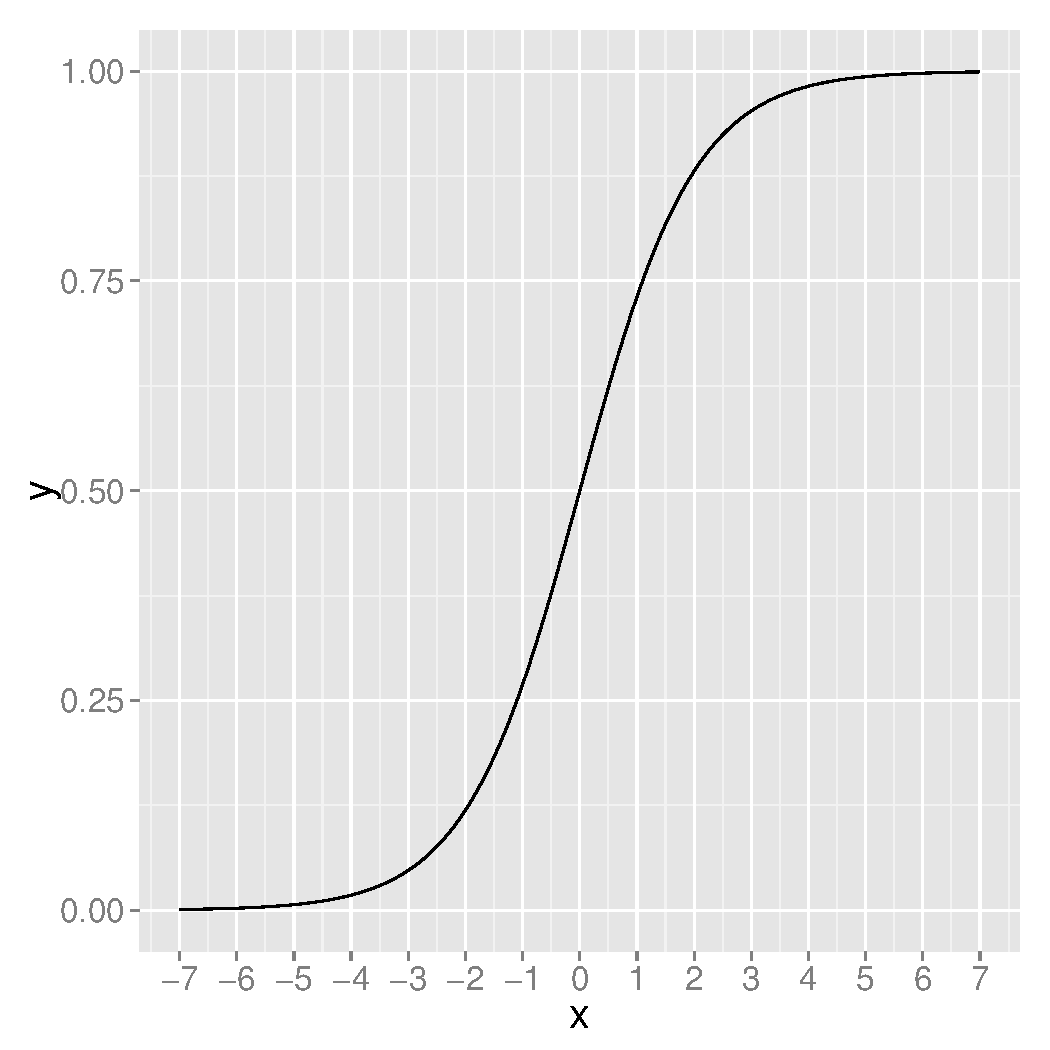
\includegraphics[width=0.45\columnwidth]{images/plot-sigmoid}\hfill{}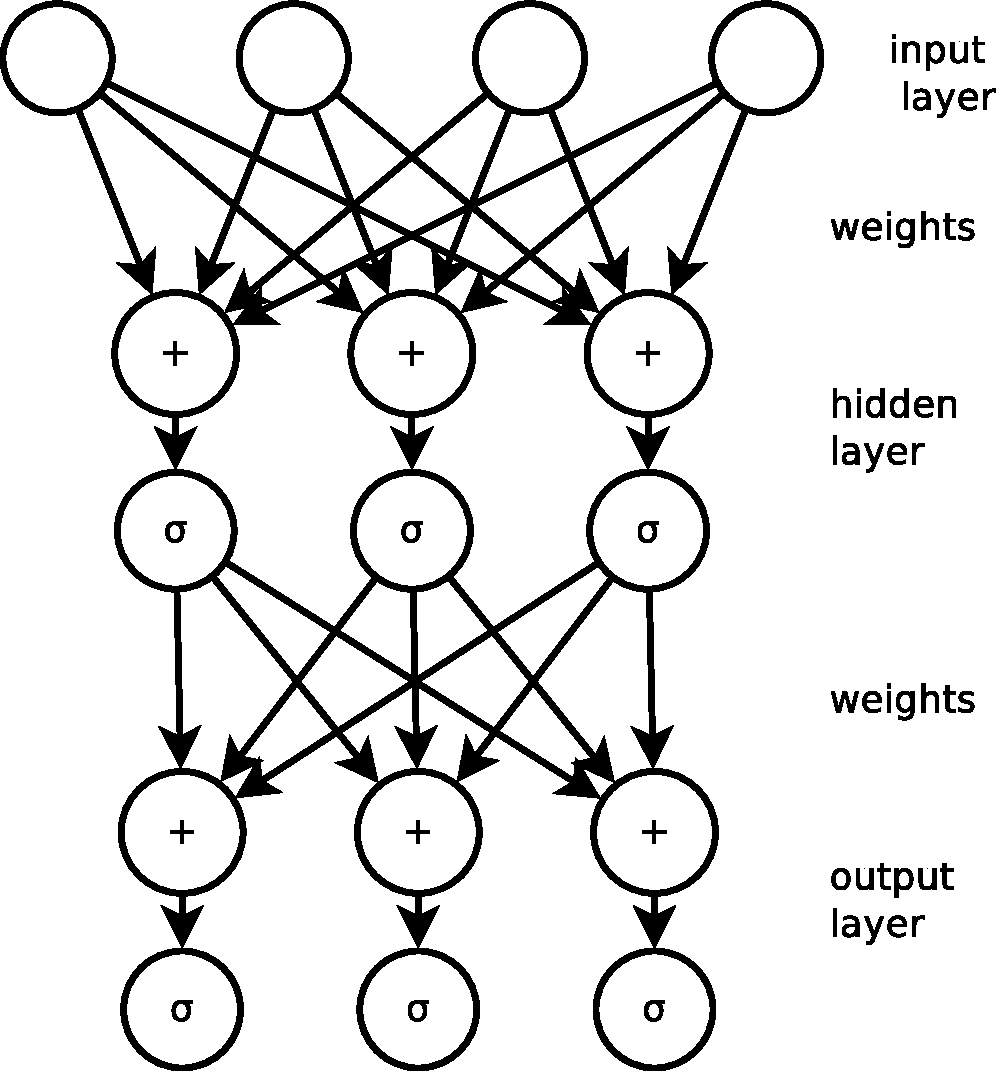
\includegraphics[width=0.45\columnwidth]{images/neuronal-network-example}
\par\end{centering}
\caption{\label{fig:sigmoid-function}Left: The sigmoid function $\sigma$.
Right: Schema of the computational steps in an artificial neural feed-forward
network\index{feed-forward neural network} from input layer to output
layer. The ``+'' nodes accumulate their input values, and the ``$\sigma$''
nodes compute the output of a neuron, to be used as input for the
next layer.}
\end{figure}

The effect of an incoming axon onto a neuron, that is, the different
types of receptors that can be present on the outside of a real dendrite,
and the effected de- or hyperpolarization of the dendrite are abstracted
away by using real-numbered weights. Weights are parameters to the
mathematical function describing the conversion of outputs of neurons
to the single input of the next connected neuron. Usually the input
$v_{i}$ of neuron $i$ is computed from the outputs of its connected
neurons $\mathbf{c_{i}}$ as in
\begin{equation}
v_{i}=b_{i}+\sum_{j\in\mathbf{c_{i}}}o_{j}w_{ij},\label{eq:input-to-a-neuron}
\end{equation}
where $b_{i}\in\mbox{\ensuremath{\mathbb{R}}}$ is the so-called \emph{bias}\index{bias of an artificial neuron}\emph{
}of neuron $i$, $\mathbf{c_{i}}$ is the vector of indices of its
in-going connected neurons, $o_{j}\in\mathbb{R}$ is the activation
of the connected neuron $j$, and $w_{ij}\in\mathbb{R}$ is the weight
of the connection going out of neuron $j$ and into neuron $i$.

In an neural network the neurons are often arranged in layers. See
the right panel of figure \ref{fig:sigmoid-function} for an example
of the structure of an artificial neural network.

\subsection{Learning in Biological Neural Networks}

Nervous systems do not only process signals, but they also learn,
that means that they adapt their signal processing over time. One
reason for this is an organism's need for a change in behavior, as
response to a changing environment.

In biological neuronal systems, this is possible by altering existing
synapses (for example by exchanging the receptors on the surface of
dendrites), or by creating and abandoning existing synapses (i.e.
connecting the axon terminals of a neuron to different neurons). There
are several known cellular mechanisms for that, among them LTP, LTD,
and PTP\cite{BermudezFederico2007}. Strengthening of the synaptic
link (that occurs within minutes and remains after hours and up to
weeks in the hippocampus of mammals) is called long-term potentiation
(LTP), while its weakening is called long-term depression (LTD). LTP
is induced by associativity of connected neurons, that means, when
a neuron contributes to the depolarization in a directly connected
neuron, the efficiency of that connection will be strengthened. The
molecular mechanisms responsible for this phenomenon are not yet completely
understood. It is known that they differ between brain regions, and
also between types of synapses in the same brain region. The cellular
mechanisms controlling these processes, and their interplay in larger
neuron ensembles are a field of active research \cite{BermudezFederico2007}.

An unproven hypothesis is that learning is local\index{locality of Hebbian learning rule},
which means that changes at a synapse only depend on the directly
connected neurons, but not on other distantly-connected neurons. This
type of local learning is called \emph{Hebbian learning}\index{Hebbian learning}.

The learning in biological neuronal systems happens seemingly automatically,
for example, migratory birds learn and remember travel paths around
the globe, without an apparent teacher. Ultimately the goals of learning
are determined by an interplay of evolution and the environment. 

\subsection{Back-propagation for Training Artificial Neural Networks\label{subsec:Back-propagation}}

The nearest analog to learning in biological neural networks is \emph{training
}artificial neural networks\index{training of artificial neural networks}.
Here, the goal is explicitly set by humans by providing training data
sets. One training sample consists of a vector of real numbers called
\emph{input patterns}\index{input pattern} and a corresponding vector
of real numbers of desired \emph{output patterns}\index{output pattern},
also called \emph{labels}\index{label}. For every input pattern in
the training data set an output pattern is defined that the learner
should compute from the input pattern. Learning is hereby facilitated
by changing the parameters of the artificial neural network.

Back-propagation is a supervised training procedure for artificial
neural networks \cite{RumelhartWilliams1988}. It learns from labeled
training samples. The parameters of the network, the weights and biases,
are adapted using \emph{gradient descent}\index{gradient descent}.
The basic idea is to set the neurons in the input layer to the input
pattern, compute the activations of neurons in the network, compute
the total error observed in the output layer using the difference
between actual and desired output, then determine how much each neuron
was ``responsible'' for the total error in the network, and finally
use it to adapt the weights and biases. This procedure is then repeated
until the network is fully trained.

Let the supervised training patterns be indexed by $p$, $x_{i,p}$
the activation of a neuron $i$ in the input layer for training pattern
$p$, and $y_{k,p}$ the desired activation of neuron $k$ in the
output layer for this training pattern.

\paragraph{Forward Pass}

The supervised training procedure first performs the \emph{forward
pass}\index{forward pass}: it sets activations $o_{i}$ in the input
layer according to the input pattern $x_{i,p}$ to be learned, computes
the activations $o_{j}$ of the hidden layers and the output layer
$o_{k}$.

(In the following, index $k$ is used for a neuron in the output layer,
and indices $j$ and $i$ for a neuron in a hidden layer or the output
layer. If the network has only one hidden layer, then index $i$ refers
to a neuron in the input layer.)

Each input neuron's output $o_{i}$ is set to a training input: 
\begin{equation}
o_{i}=x_{i,p}.
\end{equation}
The input $v_{j}$ to a hidden or output neuron is computed from the
sum of the connected neurons' outputs in the layer above (see section
\ref{subsec:Artificial-Neurons-as-Simple-Models-of-Biological-Neurons}
):
\begin{equation}
v_{j}=b_{j}+\sum_{i\in\mathbf{c_{j}}}o_{i}w_{ji},
\end{equation}
 where $b_{j}$ is the bias, $o_{i}$ is the output of a neuron in
the layer above, and $w_{ji}$ is the weight of the connection from
neuron $i$ to neuron $j$. The input $v_{j}$ is then scaled by the
sigmoid function to produce a neuron's output $o_{j}$:

\begin{equation}
o_{j}=\sigma(v_{j})=\frac{1}{1+\exp(-v_{j})}.\label{eq:sigmoid-function-2}
\end{equation}

\paragraph{Backward Pass for the Output Layer}

While in the forward pass the information flowed from input to output
layer, in the \emph{backward pass}\index{backward pass}, the information
flows from output to input layer, adjusting the weights and biases
on the way. See figure \ref{fig:Data-flow-in-back-propagation} for
an illustration of the two data flow directions.

\begin{figure}
\begin{centering}
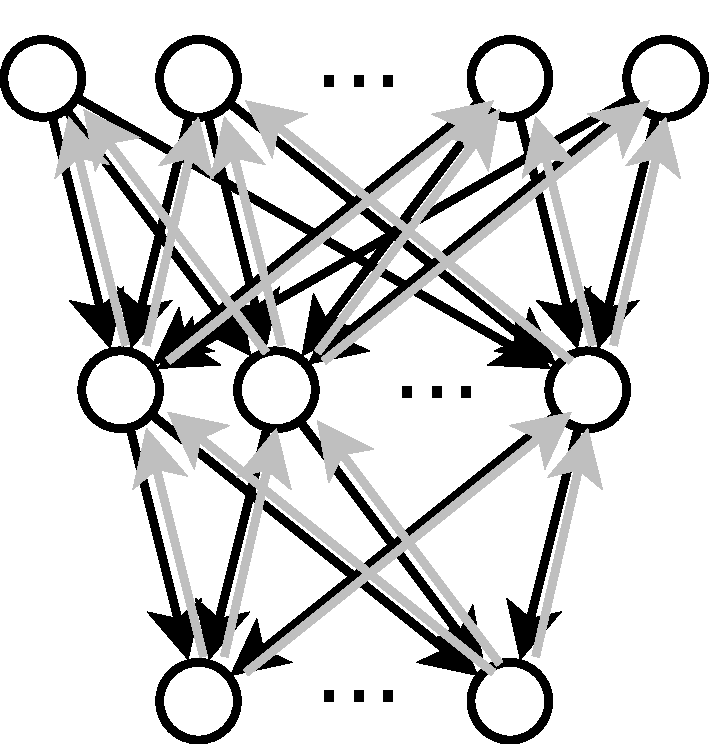
\includegraphics[width=0.34\columnwidth]{images/introduction-backpropagation-data-flow}
\par\end{centering}
\caption[Data flow in training a neural network using back-propagation.]{\label{fig:Data-flow-in-back-propagation}Data flow in training a
neural network with three layers using back-propagation. The input
layer is at the top, the hidden layer in the middle, and the output
layer at the bottom. The black arrows denote information flow during
the forward pass. Each black arrow is associated with a weight from
tail to head. The grey arrows denote information flow during the backward
pass, which propagates errors in the reverse direction.}
\end{figure}
The training procedure computes the total error $E_{total}$ of the
network, which is defined as the squared sum of differences between
actual output $o_{k}$ and desired output $y_{k}$ over all training
patterns:
\begin{eqnarray}
E_{total} & = & \sum_{p}\sum_{k}\frac{1}{2}(o_{k,p}-y_{k,p})^{2}\\
 & = & \sum_{p}E,\nonumber 
\end{eqnarray}
 where $E$ is the error of one training pattern. We further split
$E$ into a sum of errors of individual neurons $E_{k}$: 
\begin{eqnarray}
E & = & \sum_{k}\frac{1}{2}(o_{k}-y_{k})^{2}\\
 & = & \sum_{k}E_{k},\nonumber 
\end{eqnarray}
where $E_{k}=\frac{1}{2}(o_{k}-y_{k})^{2}$. To compute the contribution
of weight $w_{kj}$ to the error, the error $E$ is then differentiated
with respect to a weight $w_{kj}$ for a connection from neuron $j$
in the last hidden layer to neuron $k$ in the output layer: 
\begin{eqnarray}
\frac{\partial E}{\partial w_{kj}} & = & \frac{\partial E}{\partial o_{k}}\cdot\frac{\partial o_{k}}{\partial v_{k}}\cdot\frac{\partial v_{k}}{\partial w_{kj}}\nonumber \\
 & = & \frac{\partial\sum_{k}E_{k}}{\partial o_{k}}\cdot\frac{\partial o_{k}}{\partial v_{k}}\cdot\frac{\partial v_{k}}{\partial w_{kj}}\nonumber \\
 & = & \frac{\partial E_{k}}{\partial o_{k}}\cdot\frac{\partial o_{k}}{\partial v_{k}}\cdot\frac{\partial v_{k}}{\partial w_{kj}}\label{eq:backpropagation-error-wrt-weight-output-layer}\\
 & = & (o_{k}-y_{k})\cdot o_{k}(1-o_{k})\cdot o_{j},\nonumber 
\end{eqnarray}
 which uses that the derivative of the sigmoid function $o_{k}=\frac{1}{1+\exp(-v_{k})}$
is $\frac{\partial o_{k}}{\partial v_{k}}=o_{k}(1-o_{k})$. The derivative
of the error with respect to $b_{k}$ is
\begin{equation}
\frac{\partial E}{\partial b_{k}}=\frac{\partial E}{\partial o_{k}}\cdot\frac{\partial o_{k}}{\partial v_{k}}\cdot\frac{\partial v_{k}}{\partial b_{k}}=(o_{k}-y_{k})\cdot o_{k}(1-o_{k})\cdot1.
\end{equation}

\paragraph{Backward Pass for the Other Layers}

To perform gradient descent, we also need to update the weights and
biases for the remaining connections between hidden layers, and from
the input layer to the first hidden layer. The derivative of the error
with respect to the weight $w_{ji}$ of the connection from neuron
$i$ in a layer to neuron $j$ in the layer below (for example, from
neuron $i$ in the second last hidden layer to neuron $j$ in the
last hidden layer) is
\begin{eqnarray}
\frac{\partial E}{\partial w_{ji}} & = & \frac{\partial E}{\partial o_{j}}\cdot\frac{\partial o_{j}}{\partial v_{j}}\cdot\frac{\partial v_{j}}{\partial w_{ji}}\label{eq:backpropagation-error-wrt-weight-other-layers}\\
 & = & \frac{\partial E}{\partial o_{j}}\cdot o_{j}(1-o_{j})\cdot o_{i},\nonumber 
\end{eqnarray}
 where 
\begin{eqnarray}
\frac{\partial E}{\partial o_{j}} & = & \frac{\partial}{\partial o_{j}}\sum_{k}E_{k}\nonumber \\
 & = & \sum_{k}\frac{\partial}{\partial o_{j}}E_{k}\nonumber \\
 & = & \sum_{k}\frac{\partial E_{k}}{\partial o_{k}}\frac{\partial o_{k}}{\partial v_{k}}\cdot\frac{\partial v_{k}}{\partial o_{j}}\nonumber \\
 & = & \sum_{k}\frac{\partial E_{k}}{\partial o_{k}}\frac{\partial o_{k}}{\partial v_{k}}\cdot w_{kj},\label{eq:backpropagation-error-wrt-output-other-layers}
\end{eqnarray}
and neuron $k$ is in the layer below the layer that neuron $j$ is
in (in our example neuron $k$ is in the output layer). We take the
value for $\frac{\partial E_{k}}{\partial o_{k}}\frac{\partial o_{k}}{\partial v_{k}}$
in equation \ref{eq:backpropagation-error-wrt-output-other-layers}
above from equation \ref{eq:backpropagation-error-wrt-weight-output-layer}
when neuron $k$ is in the output layer or equation \ref{eq:backpropagation-error-wrt-weight-other-layers}
when neuron $k$ is in a hidden layer. (Neuron $k$ is named $j$
in equation \ref{eq:backpropagation-error-wrt-weight-other-layers}.)
In our example (for neuron $j$ in the last hidden layer), we take
$\frac{\partial E_{k}}{\partial o_{k}}\frac{\partial o_{k}}{\partial v_{k}}$
from the output layer: 
\begin{eqnarray}
\frac{\partial E}{\partial o_{j}} & = & \sum_{k}\frac{\partial E_{k}}{\partial o_{k}}\cdot\frac{\partial o_{k}}{\partial v_{k}}\cdot w_{kj}\\
 & = & \sum_{k}(o_{k}-y_{k})\cdot o_{k}(1-o_{k})\cdot w_{kj}.\nonumber 
\end{eqnarray}
Analogously, the derivative of $E$ with respect to $b_{j}$ is 
\begin{eqnarray}
\frac{\partial E}{\partial b_{j}} & = & \frac{\partial E}{\partial o_{k}}\frac{\partial o_{k}}{\partial v_{k}}\cdot\frac{\partial v_{k}}{\partial o_{j}}\cdot\frac{\partial o_{j}}{\partial v_{j}}\cdot\frac{\partial v_{j}}{\partial b_{j}}\\
 & = & \sum_{k}\frac{\partial E_{k}}{\partial o_{k}}\frac{\partial o_{k}}{\partial v_{k}}w_{kj}\cdot o_{j}(1-o_{j})\cdot1.\nonumber 
\end{eqnarray}

The error for each node $\frac{\partial E_{k}}{\partial o_{k}}\cdot\frac{\partial o_{k}}{\partial v_{k}}$
is thus back-propagated in reverse input direction through the hidden
layers, until all derivatives have been determined.

\subparagraph{Updating rule}

After having computed the derivatives of the error with respect to
the parameters of the network, we can perform gradient descent and
integrate these derivatives over the training patterns $p$. We update
each weight $w$ and bias $b$ using the learning rate\index{learning rate}
$\epsilon$, a small positive number:
\begin{eqnarray}
\Delta w & = & -\epsilon\sum_{p}\frac{\partial E}{\partial w}^{(p)}\\
\Delta b & = & -\epsilon\sum_{p}\frac{\partial E}{\partial b}^{(p)},\nonumber 
\end{eqnarray}
where $\frac{\partial E}{\partial w}^{(p)}$ or $\frac{\partial E}{\partial b}^{(p)}$
are the derivatives of the error with respect to a weight or bias,
when the input layer was set to training pattern $p$.

Alternatingly performing forward and backward pass and updating the
weights and biases, until the error over all training patterns $E_{total}$
is small enough, forms the complete back-propagation training procedure
of a neural network.

\paragraph{Limits of Backpropagation}

The purpose of error back-propagation is to adjust the weights of
the artificial neural network following the gradient, such that when
the current input pattern pair is presented to the network, its computed
output pattern gets closer and closer to the desired output pattern.
However, back-propagation is not able to train networks with more
than one or two hidden layers, because it is a gradient descent method
and can get stuck in poor local optima, and the error surface gets
more rugged the more hidden neurons and layers there are \cite{GoriTesi1992}.
Having artificial neural networks with more than one hidden layer
is desirable, because they can perform the same computation with less
total number of hidden nodes compared to a network with less hidden
layers. A network with one hidden layer less needs up to an exponential
factor more hidden nodes \cite{Hastad1987}.

\section{Introduction to Machine Learning}

\subsection{Supervised and Unsupervised Machine Learning}

In machine learning, there are two major types of learning: \emph{supervised}\index{supervised machine learning}
and \emph{unsupervised learning}\index{unsupervised machine learning}
\cite{Barber2012}. Both methods process training data sets that are
in matrix form: for example, in expression data, the rows usually
denote different genes or transcripts, and each column represents
an independently measured sample. (Note that in the general machine
learning literature, usually the data matrix is transposed: the columns
denote the features, and the rows the samples.) Samples usually are
tissue, blood samples, or cell line, and differ in their biological
background (e.g. cell type, gene knock-out or knock-in, cell cycle
phase) or treatment (e.g. drugs applied).

In supervised learning, for every input pattern in the data set an
output pattern is defined that the learner should compute from the
input pattern. Herein, both input and output pattern can be one- or
multi-dimensional vectors. The goal of supervised learning is to infer
a function that maps from the space of input patterns to the space
of output patterns. The output patterns are also called \emph{labels}\index{labels}.
(The fact that for every input pattern there is a defined output pattern
is termed ``the input data is labeled'').

In unsupervised learning, there is only an input data set and the
goal is to find its compact description. The output of an unsupervised
learning algorithm is the underlying structure of the data according
to the algorithm's objective function. The objective of an unsupervised
learning algorithm can range from dimensionality reduction to data
re-representation to latent variable modelling.

Examples of supervised learning algorithms are (linear or logistic)
regression, k-Nearest Neighbor (k-NN) regression, support vector machines
(SVMs), and backpropagation neural networks. Examples for unsupervised
learning algorithms are (hierarchical or kNN) clustering, self-organising
maps (SOMs), principal component analysis (PCA), and Restricted Boltzmann
Machines (RBMs).

A goal of both supervised and unsupervised learning is that the learned
rules should generalize well, i.e. previously unseen data should be
characterized correctly. The samples are therefore split into training,
validation and test data sets. The \emph{training data set}\index{training data set}
is used to train a machine learning algorithm. Some machine learning
algorithms have meta-parameters, i.e. parameters that are needed for
the algorithm, but that we are not really interested in. (An example
is the number of hidden neurons in an artificial neural network.)
The meta-parameters are optimized using the \emph{validation data
set}\index{validation data set}. At the end of training, the performance
of the machine learning algorithm must be evaluated on previously
unseen samples, the \emph{testing data set}\index{testing data set}.

\subsection{Semi-supervised Machine Learning}

An intermediate form between supervised and unsupervised machine learning
is semi-supervised learning\index{semi-supervised learning}. In contrast
to supervised machine learning, which has for every input pattern
a target output pattern, semi-supervised learning does not need a
target output pattern for every input pattern. However, in contrast
to fully unsupervised machine learning, it does need some labeled
input data sets. A common objective of semi-supervised machine learning
algorithms is to find underlying structure in all input data sets
and then use the known labels to assign labels to unlabeled input
samples. This assumes that samples close in the (high-dimensional)
input space have the same label. Another assumption is that samples
distant to each other have different labels. An example of a possible
improvement of semi-supervised classification over supervised classification
is given in figure \ref{fig:Illustration-of-semi-supervised-learning}
(adapted from \cite{Joachims1999a}). In the figure, the two-dimensional
samples are either labeled orange or blue, or unlabeled, and the task
is to (1) find a straight line that separates samples with the two
colors and (2) color the unlabeled samples. Supervised learning alone
does not take into account the unlabeled samples, while semi-supervised
learning recognizes that there are two clouds of samples, separated
by a gap, where the labeled samples from each color are on different
sides of the gap. It then draws the separating line in the middle
of the gap, and colors the unlabeled samples on the side with the
orange samples orange, and the unlabed samples on the other side blue.

\begin{figure}
\begin{centering}
A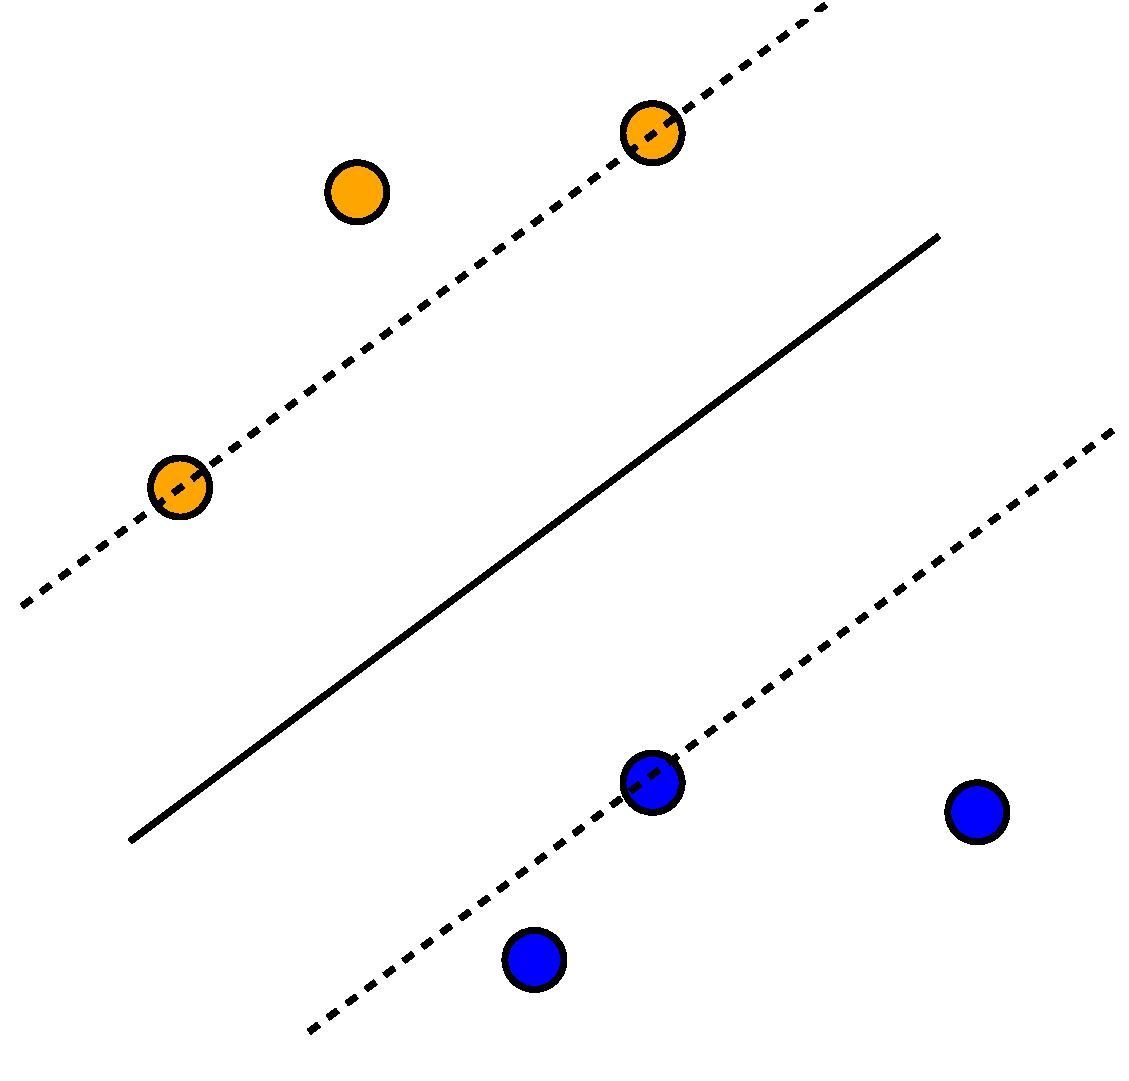
\includegraphics[width=0.3\columnwidth]{images/semi-supervised-advantage1}
B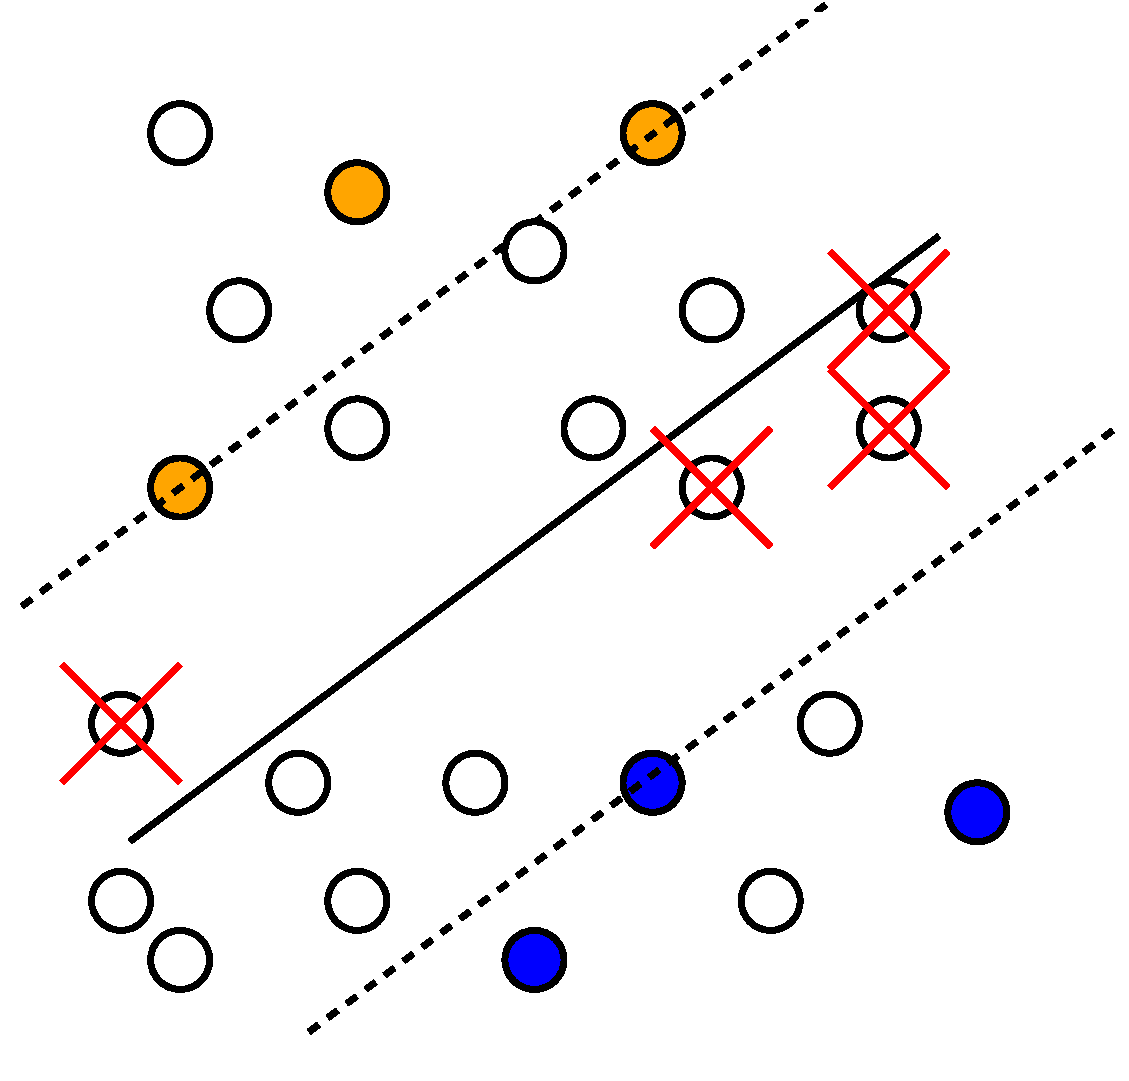
\includegraphics[width=0.3\columnwidth]{images/semi-supervised-advantage2}
C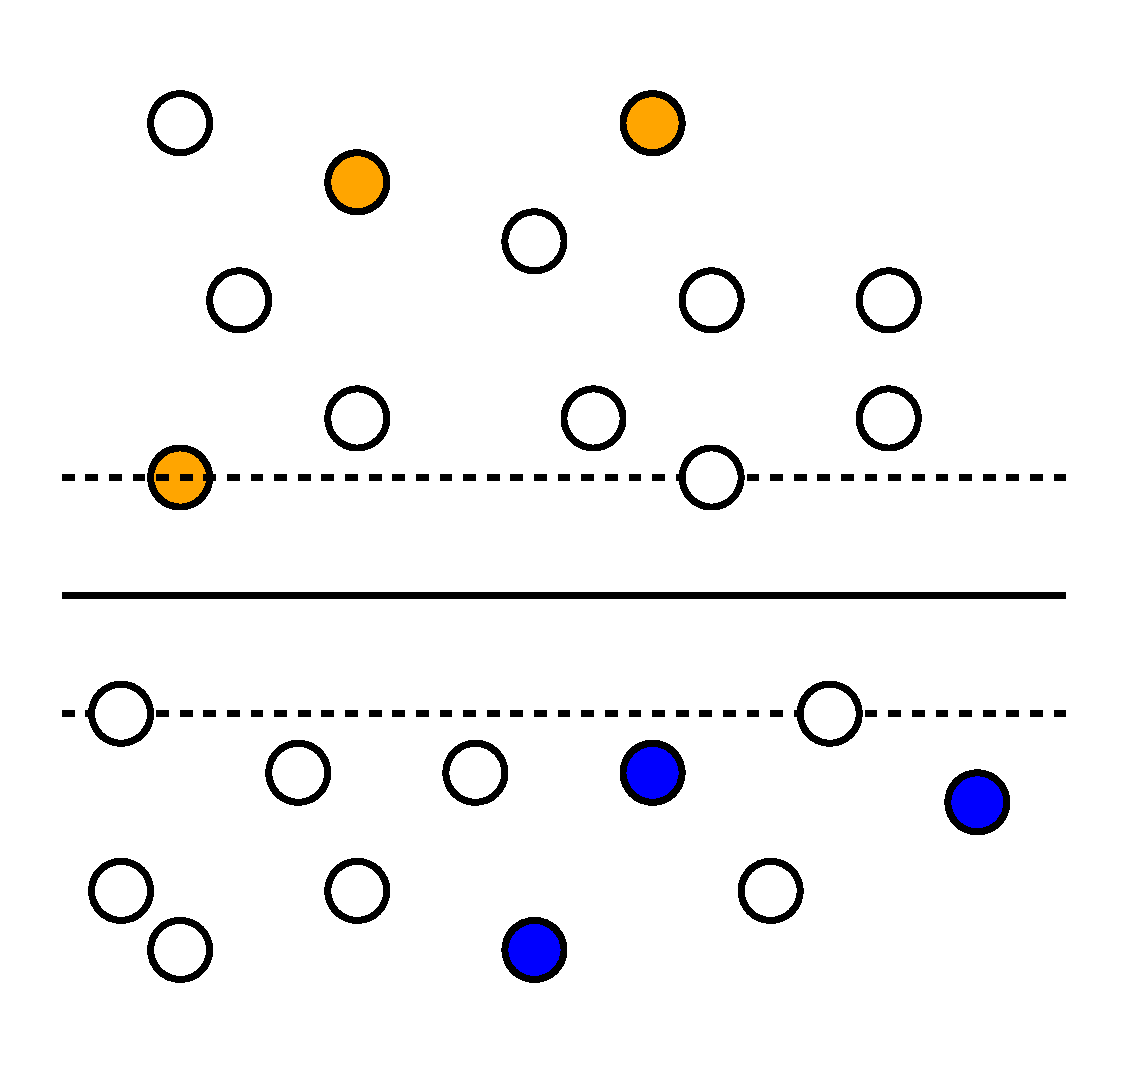
\includegraphics[width=0.3\columnwidth]{images/semi-supervised-advantage3}
\par\end{centering}
\caption[Illustration of semi-supervised learning in two dimensions.]{\label{fig:Illustration-of-semi-supervised-learning}Illustration
of semi-supervised learning in two dimensions. Each axis is a dimension.
Circles are samples; filled circles are labeled samples; unfilled
circles are unlabeled samples. The blue circles are samples with label
1, the orange circles are samples with label 2. A: Supervised SVM
learning produces a maximum-margin classifier. B: Supervised learning
ignores and probably mis-classifies some unlabeled samples (the red
crossed-out samples). C: Semi-supervised learning regards densities
of unlabeled samples and may give better results than supervised learning
on the labeled samples alone.}
\end{figure}

There are two types of semi-supervised learning: transductive and
inductive semi-supervised learning. The goal of transductive semi-supervised
learning\index{transductive semi-supervised learning} is to predict
the class labels of a pre-specified list of unlabeled input patterns,
while the goal of inductive\index{inductive semi-supervised learning}
semi-supervised learning is to find a universal rule mapping from
the space of input patterns to class labels, which could be applied
to classify unknown, future input patterns. In case unknown, future
input patterns are to be classified using transductive semi-supervised
machine learning, the whole model may have to be re-evaluated.

\subsubsection{Example Scenarios for Semi-supervised Learning}

An advantage of semi-supervised learning over supervised learning
is that it does not need labels for all input patterns, because labels
are often time-consuming or costly to acquire. For example, the Gene
Expression Omnibus data base (GEO) \cite{BarrettSoboleva2013} contains
41,379 expression data sets that were uploaded between Jan 1st, 2000,
and August 31st, 2013. Many of these are potentially usable as unlabeled
data sets in semi-supervised learning.

However in practice, many machine learning algorithms require samples
to be independently and identically distributed\index{independetly and identically distributed}
(iid\index{iid}). In an ideal world, GEO samples could be assumed
to be identically distributed within a data set. Unfortunately even
within the same GEO data set there often is systematic variation between
samples, called the \emph{batch-effect}\index{batch-effect}, caused,
for example, by different sample handling or conditions at measurement
time. Hence one either has to use samples from one data set only,
or, if one wants to use samples from different GEO data sets simultaneously,
correct for a possible batch-effect manually, or use an algorithm
that has some built-in mechanism to make such a correction.

One machine learning algorithm with such a built-in mechanism is\emph{
deep learning}\index{deep learning}, as employed in \emph{Deep Belief
Networks}\index{Deep Belief Network}\emph{ (DBNs}\index{DBN}\emph{)}
\cite{HintonTeh2006}. This machine-learning algorithm (which is unsupervised,
but can be used for supervised and semi-supervised learning) can learn
from images of objects or faces, where the objects or faces are in
different lighting conditions or are viewed from different angles
(\cite{HintonSalakhutdinov2006,KrizhevskyHinton2012,KarpathyFei-Fei2014}).
In this setting, the batch effect would be the lighting condition
or viewing angle. Such results seem to imply that DBNs are able to
abstract the images, which are given as vectors of pixels, into encodings
of relevant features and compute a classifier on these abstract features.
This can be seen as a form of batch-effect correction.

An extreme form of batch-effect correction is when all training data
are in batch 1 and all test data in batch 2. Are neural networks able
to handle such a situation? For example, suppose that batch 1 are
all face portraits (frontal view), batch 2 are half profile faces
(30 degree angle view) of \textendash{} not necessarily the same \textendash{}
people, and the task is to match faces seen from both viewing angles
to the same person. During training, semi-supervised learning would
have access to the unlabeled faces from both viewing angles, but all
the half profiles would be unlabeled. We are not aware of a study
of that setting using artificial neural networks, but a similar setting
was studied in cognitive psychology, where humans were the learners
\cite{BobakBate2015}. The participants of the study were asked to
match a given half profile to one out of 10 portraits, or indicate
that there is no matching face. The accuracy of average people was
81\%, while people who have extraordinary face recognition abilities,
so-called ``super-recognizers'', had 94\% accuracy. When there was
no matching face, average people correctly rejected the face in 65\%
of all cases, and super-recognizers did so in 92\%. For humans, the
unsupervised training would consist in seeing people's faces from
different angles during normal day-to-day activity. However, one could
argue that this training is unfair, because humans had access to the
label of many half profiles, since they often have seen a person's
portrait just moments before seeing the half profiles.

\subsection{Deep Learning}

Deep learning\index{deep learning} is a term used in artificial neural
networks with several hidden layers. The advantage of a deep network
over a network with just one hidden layer is that it can model a problem
more compactly using less hidden neurons in total, because it has
more than one intermediate computation step.

\emph{Autoencoders} and \emph{Deep Belief Networks}\index{Deep Belief Network}\emph{
}(\emph{DBNs}\index{DBN}) overcame the limitation of only a few hidden
layers \cite{BengioLarochelle2007,HintonTeh2006}. Here we give brief
overviews over both types of artificial neural network.

\paragraph{Autoencoder}

An autoencoder is a network with more than one hidden layer, whose
training is unsupervised and its objective is to reconstruct the input
in the output layer. An autoencoder starts as a three-layer network
composed of input layer, hidden layer, and output layer. This network
is trained using back-propagation. The middle hidden layer is then
copied and new hidden layer is inserted between both copies, forming
a five-layer-network. The newly added parameters of this network are
the same in number compared to a three-layer network, which can be
trained using back-propagation. Hence, training the five-layer-network
using back-propagation also works, and adding a new hidden layer in
the middle can be repeated.

\paragraph{Deep Belief Network}

Training a Deep Belief Network is separated into a pre-training phase
and a fine-tuning phase. The pre-training phase is unsupervised. It
starts with a network consisting of one input layer and a hidden layer.
This pair of  layers is called a \emph{Restricted Boltzmann Machine}\index{Restricted Boltzmann Machine}
(RBM\index{RBM}). There is an accompanying unsupervised training
procedure called \emph{contrastive divergence}\index{contrastive divergence}
which finds weights between these layers. After training the RBM,
hidden layers are iteratively added on top of the RBM, and the new
weights between layers are initialized and pre-trained using contrastive
divergence. While the pre-training phase is unsupervised, the fine-tuning
phase can be unsupervised as well as supervised. After training, the
multiple-hidden-layer-network forms a generative artificial neural
network called a Deep Belief Network.

\section{Overview of Own and Related Work}

We used autoencoders, Deep Belief Networks, and Transductive Support
Vector Machines on expression data to predict whether breast cancer
patients will show pathologic complete response to chemotherapy or
residual disease. The expression data are high-dimensional ($\approx22,000$
genes) and we use a relatively large data set ($\approx500$ patients).

\subsection{Motivations for Using Deep Belief Networks on Transcriptomic Data}

The motivations for using Deep Belief Networks on transcriptomic data
come from those networks' successes when used on image data. In the
hand-written digit classification and graphical object recognition
data sets on which the deep artificial neural networks were developed,
they are among the best-performing predictors.

\subsubsection{The ImageNet Large Scale Visual Recognition Challenge}

An example for the success of deep neural network is image classification
in the ImageNet Large Scale Visual Recognition Challenge \cite{RussakovskyFeiFei2015}.
It is a yearly contest, wherein participants are given around 1.2
million training images. Each training image is labeled with one of
$1,000$ possible object categories describing the main object appearing
in the image, for example ``trumpet'' or ``butterfly''. After
training an image classification algorithm, each contestant must compute
up to $5$ labels for each of $100,000$ test images. Each test image
has a single label, which is kept hidden by the contest organizer.
A test image is scored as correctly classified if the correct label
appears in the (up to $5$) labels submitted by the contestant. (Up
to 5 labels may be submitted because for example a street scene may
contain, besides the correct ``car'' label also street signs and
drivers.) Finally, the accuracy of a contestant is computed as the
average fraction of correctly classified test images.

There have been notable improvements in the accuracy of the winning
contestant, starting in 2012. In the last years, all top contestants
have moved to using deep neural networks. See table \ref{tab:ILSVRC-Test-set-accuracies}
for the winning contestants between 2010 and 2014. Significant differences
before and after 2012 are the usage of neural networks directly on
the image pixel data, and not using pre-computed image features in
a supervised learning algorithm like a Support Vector Machine.

\begin{table}
\begin{centering}
\begin{tabular}{|c|c|c|c|}
\hline 
Year & Winner & Accuracy & Technique\tabularnewline
\hline 
\hline 
2010 & NEC & 71.8\% & SIFT and LBP image features classified by SVM\tabularnewline
\hline 
2011 & XRCE & 74.2\% & image signatures classified by one-vs-all SVMs\tabularnewline
\hline 
2012 & SuperVision & 83.6\% & deep convolutional neural network\tabularnewline
\hline 
2013 & Clarifai & 88.3\% & deep convolutional neural networks averaged\tabularnewline
\hline 
2014 & GoogLeNet & 93.3\% & deep convolutional neural network\tabularnewline
\hline 
\end{tabular}
\par\end{centering}
\caption[Test set accuracies and techniques of winning contestants in the ImageNet
Large Scale Visual Recognition Challenge from 2010-2014.]{\label{tab:ILSVRC-Test-set-accuracies}Test set accuracies and techniques
of winning contestants in the ImageNet Large Scale Visual Recognition
Challenge from 2010-2014. Column ``Year'' is the year of the contest,
``Winner'' the team name of the winner of this year, ``Accuracy''
the test set accuracy of the winner's submission, and ``Technique''
a summary of the winner's algorithm technique. SVM, support vector
machine.}
\end{table}

\subsubsection{Highly Correlated Inputs}

We will now discuss similarities between image classification and
expression data classification.

Both underlying distributions \textendash{} of images and of expression
data \textendash{} have many correlated features. For images, adjacent
pixels often display the same object and have therefore correlated
values. In some face recognition tasks for example, the faces are
scaled and translated so that the centers of both eyes and mouth are
aligned in different faces. There will be highly correlated pixels
for areas of the image where the cheeks and lips usually are. If you
use the pixels of the whole image as input to the neural network,
the corresponding input nodes will be highly correlated as well.

For transcriptomic data, one almost always observes many correlated
genes. The correlations can be due to many genes being regulated by
the same transcription factor \cite{TornowMewes2003,KlebanovYakovlev2007}.

\subsubsection{Deep Belief Networks Find Correlated Nodes}

Deep Belief Networks can group correlated input nodes. The network
can do this by increasing the weights from the correlated group to
a single hidden node, and decreasing the weights from the group to
all other hidden nodes. The hidden node becomes the representative
of the correlated group of input nodes. This is a form of abstraction
and dimensionality reduction. The hidden node will only be active
if many of its highly-weighted input nodes are active and only few
of its negatively-weighted input nodes are active. Repeated application
of this principle of abstraction in deeper and deeper hidden layers
allows the Deep Belief Network to form more and more abstract representations
of its input.

In face recognition for example, an abstract representation might
have a single value for the size of the lips. In expression data,
a single node in an abstract representation might encode the activity
of a gene module.

\subsubsection{Transductive Support Vector Machine}

We compare the artificial neural network approach with another, older,
and established semi-supervised method, the Transductive Support Vector
Machine (TSVM) \cite{Joachims1999}. Despite the name, it supports
transductive as well as inductive learning. A standard Support Vector
Machine searches for a decision boundary such that the margin between
samples with differing labels is maximal (see figure \ref{fig:Illustration-of-semi-supervised-learning}).
The TSVM seeks a labeling of the unlabeled samples so that the decision
boundary has the maximal margin between all samples with differing
classes. 

\subsection{Previous Work: Gene Expression Inference With Deep Learning\label{subsec:Previous-Work:Gene-Expression-Inference-with-Deep-Learning}}

Very recently, \cite{ChenXie2015} published work on compressing expression
data into fewer dimensions on a large scale using deep learning. The
motivation for this work was that principal component analysis found
that $943$ ``landmark'' genes can capture about 80\% of the information
in the CMAP data set. This prompted the development of the ``L1000
Luminex bead technology'', which measures the expression of these
$943$ genes at a low cost, and computationally infers the remaining
$\approx21,000$ genes. \cite{ChenXie2015} worked on improving this
computational inference step.

Input data were all $\approx111,000$ genome-wide expression profiles
from the GEO database of Affymetrix microarrays, which were partitioned
into training, validation, and testing data sets. For each sample,
the same subset of $943$ landmark genes was chosen and $9,520$ other
genes were predicted from the landmark genes. This is different from
our work, because we classified breast cancer samples using gene expression
levels, while \cite{ChenXie2015} did regression of gene expression
levels using other gene expression levels.

\cite{ChenXie2015}'s artificial neural network architecture had between
$1$ and $3$ hidden layers with either $3,000$, $6,000$, or $9,000$
nodes. It had 943 input expression values (one for each landmark gene),
and a total of $9,520$ output expression values (one for each gene
to be predicted). In addition to the (non-linear) neural network,
they evaluated linear regression with no regularization, L1-, and
L2-regularization.

\cite{ChenXie2015} also evaluated k-Nearest Neighbor \index{k-Nearest Neighbor}(kNN\index{kNN}).
During training, they determined a number, $k$, of landmark genes
with expression value closest to each target gene $i$ (let's call
this set of genes $knn_{i}$) in the training data set. During testing,
they predicted the expression value of the target gene $i$ as the
average of the gene's $knn_{i}$ expression values in the testing
data set. The optimal $k$ (number of genes to average over) was chosen
based on a validation data set.

The input values were quantile normalized expression values between
4 and 15. The models were ranked according to the average prediction
errors over all 9,520 target genes.

k-Nearest Neighbor performed worst, with an average prediction error
of $0.5866$. Linear regression without regularization and with L2-regularization
both had an average prediction error of $0.3784$. Linear regression
with L1-regularization had an average prediction error of $0.3782$.
As the three linear regression models performed about equally well,
regularization did not improve linear regression. The neural network-based
average prediction errors were between $0.3421$ and $0.3204$, with
the network having $3$ hidden layers of size $9,000$ and $10\%$
dropout rate performing best. (\emph{Dropout }is a regularization
technique for neural networks, explained in section \ref{subsec:Dropout}.)
Because the input expression values were between $4$ and $15$, an
average prediction error of $0.3204$ implies an average error of
about $3\%$ on the GEO dataset.

In another dataset, \cite{ChenXie2015} again predicted $9,520$ genes
from the $943$ landmark genes, but used the GEO dataset for training,
the $1,000$ Genomes data for validation \cite{LappalainenPedro2013},
and GTEx data for testing \cite{ArdlieLek2015}. Learning in this
data set is harder since the training, validation, and testing data
sets are measured using different expression measurement technologies,
and therefore prone to the batch-effect. Nevertheless, the performance
ranking of the methods was the same, but worse than the data set without
batch-effect. KNN scored worst, with an average prediction error of
$0.6520$. Linear regression with L1-regularization had an average
prediction error of $0.5667$. Linear regression without regularization
and with L2-regularization both had an average prediction error of
$0.4702$. The artificial neural networks all scored consistently
better than KNN and linear regression, with the artificial neural
network with $2$ hidden layers of size $9,000$, and $25\%$ dropout
rate having the lowest prediction error of $0.4393$ (which is equivalent
to a relative error of $4\%$). On the validation data set, the average
prediction error was $0.7467$, which is a relative error of $6.8\%$.
This shows that artificial neural networks are capable of processing
input from multiple sources, with an acceptable gain in error. We
had a similar result, in section \ref{sec:Unsupervised-Reconstruction-of-Expression-Values}.


\cleardoublepage{}

\part{Methods}

Here we will introduce the methods used to train deep neural networks,
as applied in the results part.

\section{Notation}
\begin{description}
\item [{Random~variable,~Node}] Random variables and nodes are written
upper-case. For example: $X$ or $N_{4}$.
\item [{Value,~Scalar~Variable}] The value of a random variable and a
scalar variable are written lower-case. For example, the value of
random variable $X$ is written $x$, and $i$ is a scalar.
\item [{Vector,~Set}] Vectors or sets are written in bold font. For example,
the vector $\mathbf{X}$ represents e.g. the random variables $\{X_{1},X_{2},X_{3}\}$.
And the vector $\mathbf{x}$ stands for e.g. the value $\{x_{1},x_{2},x_{3}\}$
of the variable $\mathbf{X}$.
\end{description}

\section{Machine Learning}


\subsection{Generative and Discriminative Models}

An often-cited quote by \cite{Vapnik1998} is: ``If you possess a
restricted amount of information for solving some problem, try to
solve the problem directly and never solve a more general problem
as an intermediate step. It is possible that the available information
is sufficient for a direct solution but is insufficient for solving
a more general intermediate problem.''

A generative model\index{generative model} is such a more general
problem: its aim is to model the input data set such that hypothetical
samples can be generated from the model which might as well be found
in the original input data set. A discriminative model\index{discriminative model}
on the other hand receives the input samples and models the output
from these inputs. Usually the outputs have lower dimension.

Restricted Boltzmann Machines and Deep Belief Networks are both generative
models, while a neural network supervisedly trained with back-propagation
is a discriminative model. In a discriminative model, the parameters
(weights and biases) specify the class label of a training sample.
In a generative model, the parameters need to encode the whole sample.
The number of bits required to specify the class label is much smaller
than the number of bits required to specify a whole training sample
\cite{Hinton2010}.

Another advantage of a generative model is that one can draw samples
from its distribution (``generate samples'') to easily find out
what the model has learned. In a discriminative model, this can be
substantially harder. Consider for example a classifier network trained
with back-propagation that decides whether an image shows a red ball
(output: true or false). The decision function of the network is a
complicated function of all input pixels. Therefore it can be hard
to determine the property an unseen image must have so that the network
would classify it as containing a red ball. Due to their greater generality,
generative models have the disadvantage that they are slower than
discriminative models. As \cite{HintonTeh2006} note, however, the
class of too computationally intensive models is being eroded by Moore's
Law.

We will discuss the established Support Vector Machines, Graphical
Models, several artificial neural networks, Restricted Boltzmann Machines,
and Deep Belief Networks.

\subsection{Support Vector Machines}

Here we review supervised and transductive Support Vector Machines\index{Support Vector Machine}
(SVMs\index{SVM} and TSVMs\index{TSVM}).

\subsubsection{Supervised Support Vector Machines}

A linear SVM\index{supervised SVM} separates data points into two
distinct classes using the hyperplane
\[
\mathbf{w}\cdot\mathbf{x}+b=0,
\]
 where $\mathbf{w}\in\mathbb{R}^{n}$ is the vector perpendicular
to the plane, $\mathbf{x}\in\mathbb{R}^{n}$ is a point on the plane,
and \textbf{$b\in\mathbb{R}$} is the distance to the origin (in units
of length $-\left\Vert \mathbf{w}\right\Vert $) \cite{StatnikovGuyon2011}.
The hyperplane is defined in the $n$-dimensional space in which the
samples lie, each sample having $n$ features. For a specific hyperplane
defined by $\mathbf{w}$ and $b$ and a sample $\mathbf{x}$, one
can calculate the distance $d$ between $\mathbf{x}$ and the hyperplane
using
\[
d=\mathbf{w}\cdot\mathbf{x}+b.
\]
In particular, the sign of $d\in\mathbb{R}$ is called the class of
$\mathbf{x}$.

\paragraph{Training a Hard-margin SVM}

When training a SVM by providing binary class labels $y_{i}\in\{-1,1\}$
for all training samples $\mathbf{x_{i}}$, the hyperplane is constructed
such that it separates the two classes and that it has the largest
possible distance (\index{margin}\emph{margin}) to border-line samples
(\index{support vectors}\emph{support vectors}). Learning a hard-margin
SVM means finding a $\mathbf{w}$ so that its length is minimal
\begin{equation}
\mbox{minimize }\frac{1}{2}\left\Vert \mathbf{w}\right\Vert ^{2}\label{eq:hard-margin-SVM-min-w}
\end{equation}
subject to the condition that all samples are classified correctly
by $\mathbf{w}$, $b$. Hence, the constraints 
\begin{equation}
y_{i}(\mathbf{w}\cdot\mathbf{x_{i}}+b)-1\geq0,\label{eq:hard-margin-SVM-constraints}
\end{equation}
(where $y_{i}$ is the true class of sample $i$) must be fulfilled
for all samples $i$. The two equations \ref{eq:hard-margin-SVM-min-w}
and \ref{eq:hard-margin-SVM-constraints} are called the ``primal
formulation of linear SVMs''. This formulation can be solved by \emph{convex
quadratic programming}\index{quadratic programming} with $n$ variables,
where $n$ is the number of features. Using Lagrange multipliers \cite{StatnikovGuyon2011},
the primal formulation can be rewritten into the equivalent ``dual
formulation'':
\begin{eqnarray}
\mbox{minimize } &  & \sum_{i}^{N}\alpha_{i}-\frac{1}{2}\sum_{i,j}^{N}\alpha_{i}\alpha_{j}y_{i}y_{j}\mathbf{x_{i}}\mathbf{x_{j}}\label{eq:hard-margin-SVM-dual-formulation-min-w}\\
\mbox{subject to } &  & \alpha_{i}\geq0\mbox{ and }\sum_{i}^{N}\alpha_{i}y_{i}=0,\nonumber 
\end{eqnarray}
where the $\alpha_{i}$s are the $N$ variables to be solved by quadratic
programming, and $N$ is the number of samples. After computing the
solution for the dual formulation, the $\mathbf{w}$-vector is given
in terms of the $\alpha_{i}$: $\mathbf{w}=\sum_{i}^{N}\alpha_{i}y_{i}\mathbf{x_{i}}$
and the distance from the origin is $b=y_{i}-\mathbf{w}\mathbf{x_{i}}$,
for any sample $i$ which has $\alpha_{i}\neq0$ \cite{BurbidgeBuxton2001}.
The classifier is then $f(\mathbf{x})=sgn(\sum_{i}^{N}\alpha_{i}y_{i}\mathbf{x_{i}}\mathbf{x}+b)$.

If there is no solution, i.e. a separating hyperplane does not exist,
one can do two things:
\begin{itemize}
\item make the margin a soft margin, i.e. allow some training samples to
be misclassified.
\item implicitly map samples into a higher dimensional space where a separating
hyperplane exists. This implicit mapping is called the \emph{kernel
trick}.
\end{itemize}
Both strategies will be described in the following.

\paragraph{Training a Soft-margin SVM}

A soft-margin SVM is learned by introducing \index{slack variables}\emph{slack
variables }$\xi_{i}\geq0$ in the primal formulation:
\begin{eqnarray*}
\mbox{minimize } &  & \frac{1}{2}\left\Vert \mathbf{w}\right\Vert +C\sum_{i}^{N}\xi_{i}\\
\mbox{subject to } &  & y_{i}(\mathbf{w}\cdot\mathbf{x_{i}}+b)\geq1-\xi_{i}\mbox{ for }i=1,\dots,N
\end{eqnarray*}
and in the dual formulation:
\begin{eqnarray}
\mbox{minimize } &  & \sum_{i}^{N}\alpha_{i}-\frac{1}{2}\sum_{i,j}^{N}\alpha_{i}\alpha_{j}y_{i}y_{j}\mathbf{x_{i}}\mathbf{x_{j}}\label{eq:soft-margin-SVM-dual-formulation-min-w}\\
\mbox{subject to } &  & 0\leq\alpha_{i}\leq C\mbox{ and }\sum_{i}^{N}\alpha_{i}y_{i}=0\mbox{ for }i=1,\dots,N,\nonumber 
\end{eqnarray}
where $C>0$ is a meta-parameter that controls trading off a small
margin size $\left\Vert \mathbf{w}\right\Vert $ for allowing misclassifications
of training samples. Many SVM implementations have a default of 1.

\paragraph{Kernel Trick}

\index{kernel trick}The samples can be mapped into a higher-dimensional
space where a separating hyperplane exists or has a larger margin.
Mapping vectors $\mathbf{x}$ into a higher-dimensional space $\Phi(\mathbf{x})$
explicitly requires computing all dimensions, which is time-consuming
or impossible for infinite-dimensional spaces.

However, in the dual formulations in equations \ref{eq:hard-margin-SVM-dual-formulation-min-w}
and \ref{eq:soft-margin-SVM-dual-formulation-min-w} above, the sample
vectors $\mathbf{x_{i}}$ only occur together in a scalar product
with another sample $\mathbf{x_{j}}$. The mapping can be done implicitly
by not computing $\Phi(\mathbf{x_{i}})$ and $\Phi(\mathbf{x_{j}})$,
but by defining a \emph{kernel }function $K$ that computes the scalar
product $\Phi(\mathbf{x_{i}})\cdot\Phi(\mathbf{x_{j}})$ directly:
\[
K(\mathbf{x_{i}},\mathbf{x_{j}}):\mathbb{R}^{n}\times\mathbb{R}^{n}\rightarrow\mathbb{R}.
\]
Calculating $K$ is much cheaper than computing $\Phi(\mathbf{x_{i}})$,
$\Phi(\mathbf{x_{j}})$. Not every function can be a kernel, it has
to satisfy the Mercer conditions: for all square-integrable functions
$g(x)$ the integral 
\[
\int\int K(\mathbf{x_{i}},\mathbf{x_{j}})g(\mathbf{x_{i}})g(\mathbf{x_{j}})d\mathbf{x_{i}}d\mathbf{x_{j}}\geq0
\]
 must be non-negative. Otherwise, the quadratic programming problem
may not have a solution \cite{StatnikovGuyon2011}.

\subsubsection{Transductive Support Vector Machines\label{subsec:Transductive-Support-Vector-Machines}}

A Transductive SVM \index{transductive SVM} (TSVM) \index{TSVM}
is a semi-supervised version of a SVM \cite{Joachims1999a}. In addition
to $N$ training samples $\mathbf{x_{i}},$ and their class labels
$y_{i}$, we now know $N^{*}$ test samples $\mathbf{x_{j}^{*}}$
without labels. The objective of training a TSVM is to find class
labels $y_{j}^{*}$ for the test samples, such that a separating hyperplane
between the positive and negative test and training samples has minimal
length
\begin{eqnarray*}
\mbox{minimize } &  & \frac{1}{2}\left\Vert \mathbf{w}\right\Vert +C\sum_{i}^{N}\xi_{i}+C^{*}\sum_{j}^{N^{*}}\xi_{j}^{*}\\
\mbox{subject to } &  & y_{i}\mathbf{w}\cdot\mathbf{x_{i}}+b\geq1-\xi_{i}\mbox{ for }i=1,\ldots,N\\
 &  & y_{j}^{*}\mathbf{w}\cdot\mathbf{x_{j}^{*}}+b\geq1-\xi_{j}^{*}\mbox{ for }j=1,\ldots,N^{*}\\
 &  & \xi_{i}>0\mbox{ for }i=1,\ldots,N\\
 &  & \xi_{j}^{*}>0\mbox{ for }j=1,\ldots,N^{*},
\end{eqnarray*}
where $C$ allows trading off margin size for misclassification errors
of training samples (as for the supervised SVM), and $C^{*}$ controls
the influence of test samples. If $C^{*}$ is zero, the formulation
above is equivalent to the inductive case.

Choosing class labels $y_{j}^{*}$ for the test samples $\mathbf{x_{j}^{*}}$
must be done before solving the quadratic programming problem, otherwise
it is not convex anymore (see \cite{CollobertBottou2006}). \cite{Joachims1999a}
does this by starting with an inductive SVM, i.e. setting $C^{*}$
to zero, and classifying the test samples $\mathbf{x_{j}^{*}}$ to
obtain class labels $y_{j}^{*}$. Then he proceeds by incrementing
$C^{*}$ while swapping two test samples' class labels if the objective
function decreases. When $C^{*}$ has reached a user-defined threshold,
training stops and the current test sample labels $y_{j}^{*}$, and
the separating hyperplane defined by the parameters $\mathbf{w}$
and $b$\textbf{ }are returned.

\cite{Joachims1999a} notes that it is the co-occurrence of features
that the transductive SVM exploits to transduce labels from training
samples to test samples. For example, if a cluster of features always
has a certain pattern in a group of samples containing mostly positively
labelled training samples, then test samples showing that same feature
pattern will likely also be positively labelled.

Figure \ref{fig:transductive-feature-co-occurrence} is adapted from
\cite{Joachims1999a}. It shows samples and features. Suppose sample
A and F are given as training samples, with A labeled ``positive''
and F labeled ``negative''. Samples B-E are given as test samples
and we have to label them. Transductive learning can use the co-occurrence
of features 1-3, and the co-occurrence of features 4-6 to label samples
B and C ``positive'' and samples D and E ``negative''. Although
feature 3 does not occur in sample A, sample C belongs to the ``positive''
class because sample B links samples A and C, by having features 1
and 3 present simultaneously. Feature 7 has the same value in all
samples and cannot contribute to the labeling.

\begin{figure}
\begin{centering}
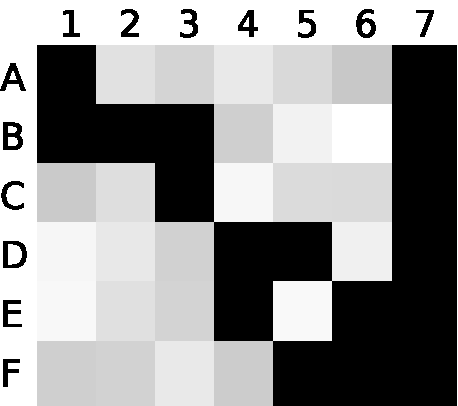
\includegraphics[width=0.35\columnwidth]{images/TSVM-co-occurrence-pattern}
\par\end{centering}
\caption[Example of the co-occurrence of features that transductive learning
can exploit.]{\label{fig:transductive-feature-co-occurrence}Example of co-occurrence
of features (columns, 1-7) that transductive learning can exploit
to label samples (rows, A-F). (See text.)}
\end{figure}

\section{Graphical Models}

\subsection{Graphs}

In the following we will define some graph nomenclature.

A \emph{graph}\index{graph} is a tuple $G=(\mathbf{N},\mathbf{E})$
of nodes $\mathbf{N}$ and edges $\mathbf{E}$. An \emph{edge}\index{edge}
$\mathbf{E}\ni E=(N_{1},N_{2})$ consists of a pair of nodes $N_{1}$
and $N_{2}$. Two nodes $N_{1}$ and $N_{2}$ connected by an edge
are called \emph{neighbors}\index{neighbor}. A \emph{complete graph}\index{complete graph}
is a graph with an edge $E=(N_{1},N_{2})$ for every distinct pair
of nodes $\mathbf{N}\ni N_{1}\neq N_{2}\in\mathbf{N}$.

An edge can be \emph{directed}\index{directed edge} or \emph{undirected}\index{undirected edge},
which means that the edge $(N_{1},N_{2})$ is either distinct from
the edge $(N_{2},N_{1})$ or they are the same. If all edges of a
graph are directed, then the graph is called a \emph{directed graph}\index{directed graph};
if all edges are undirected, then the graph is called an \emph{undirected
graph}\index{undirected graph}. In a directed edge $E=(P,C)$, also
written as $P\rightarrow C$, $P$ is called the \emph{parent}\index{parent}
and $C$ the \emph{child}\index{child}.

A \emph{path}\index{path} is an ordered list of edges $\mathbf{P}=[E_{1},E_{2},\dots,E_{n}]$,
so that the child of the previous edge is the parent of the next edge:
If $E_{i}=(P_{i},C_{i})$ and $E_{i+1}=(P_{i+1},C_{i+1})$, then $C_{i}=P_{i+1}$.
In the path $\mathbf{P}$, $P_{p}$ is called \emph{ancestor}\index{ancestor}
of $C_{c}$ if $p\leq c$, and $C_{c}$ is called  \emph{descendant}\index{descendant}
of $P_{p}$ if $p\leq c$. If the child $C_{j}$ of any edge $E_{j}$
in $\mathbf{P}$ is equal to the parent $P_{i}$ of the same or a
previous edge (i.e. $i\leq j$), then the sub-path $\mathbf{C}=[(P_{i},C_{i}),(P_{i+1},C_{i+1}),\dots,(P_{j},C_{j})]$
is called a \emph{cycle}\index{cycle}.

A \emph{directed acyclic graph}\index{directed acyclic graph} (DAG\index{DAG})
is a directed graph that does not contain directed cycles.

A \emph{clique}\index{clique} in an undirected graph is a subset
of nodes $\mathbf{N_{C}}\subset\mathbf{N}$, such that every pair
of nodes in the clique $N_{1},N_{2}\in\mathbf{N_{C}}$ has an edge
in the graph: $(N_{1},N_{2})\in\mathbf{E}$. A \emph{maximal clique}\index{maximal clique}
is a clique where there are no nodes that can be added to it so that
the resulting set of nodes is still a clique.

A set of nodes $\mathbf{N_{A}}\subset\mathbf{N}$ is \emph{separated}\index{separation of nodes}
from a set of nodes $\mathbf{N_{B}}\subset\mathbf{N}$ by a set of
nodes $\mathbf{N_{S}}\subset\mathbf{N}$, if it is impossible to go
(along the edges $\mathbf{E}$ of the graph) from a node $N_{1}\in\mathbf{N_{A}}$
to a node $N_{2}\in\mathbf{N_{B}}$ without passing through any of
the nodes in $\mathbf{N_{S}}$.

\subsection{Definition of Graphical Models}

Graphical models encode a factorization of a joint probability distribution
with the help of a graph. Each node of the graph corresponds to a
random variable of the joint probability distribution. The (union
of the) edges of the graph encode the conditional probability distributions.
Missing edges encode conditional independencies. The graph, together
with probability functions over the structural elements of the graph
is equivalent to the joint probability distribution.

Figure \ref{fig:Example-of-a-graphical-model} is an example of a
(directed) graphical model. The random variables are \textbf{$\mathbf{Sun}$},
$\mathbf{Clouds}$, \textbf{$\mathbf{Temperature}$}, and \textbf{$\mathbf{Icecream}$}.
Each variable has two possible values, for example $\mathbf{Sun}$
can be either ``S+'' or ``S-''. The tables below $\mathbf{Sun}$
and $\mathbf{Clouds}$ are called the priors, and the tables below
$\mathbf{Temperature}$ and $\mathbf{Icecream}$ are each conditional
probability distributions. The graph, together with the priors and
the conditional probability distributions, encodes the joint probability
distribution. For example, the first entry in the joint probability
distribution table is $P(\mathbf{Sun}=\mbox{S+},\mathbf{Clouds}=\mbox{C+},\mathbf{Temperature}=\mbox{T+},\mathbf{Icecream}=\mbox{I+})=$$P(\mathbf{Sun}=\mbox{S+})*P(\mathbf{Clouds}=\mbox{C+})*P(\mathbf{Temperature}=\mbox{T+}\mid\mathbf{Sun}=\mbox{S+},\mathbf{Clouds}=\mbox{C+})$$*P(\mathbf{Icecream}=\mbox{I+}\mid\mathbf{Temperature}=\mbox{T+})$$=0.5*0.5*0.7*0.7=0.1225.$
\begin{figure}
\begin{centering}
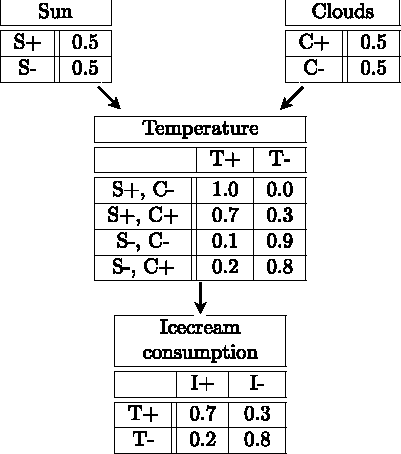
\includegraphics{images/graphical-model-example}
\par\end{centering}
\caption[Example of a graphical model.]{\label{fig:Example-of-a-graphical-model}Example of a graphical model. }
\end{figure}

\paragraph{Directed and Undirected Graphical Models}

In the following, we will introduce and discuss directed graphical
models and undirected graphical models. Directed graphical models
are also called \emph{Bayesian networks}\index{Bayesian network}
or \emph{Belief Networks}\index{Belief network}, and undirected graphical
models are also called \emph{Markov Random Fields}\index{Markov Random Field}
or \emph{Markov Networks}\index{Markov network}\footnote{There is also an unification of Bayesian networks and Markov random
fields, i.e. a graphical model that can have both directed and undirected
edges. These networks are called \emph{chain graphs} , or \emph{partially
directed acyclic graphs} and are not discussed here.}. We will consider only models with discrete random variable values.

\subsubsection{Undirected Graphical Models\label{par:Hammersley-Clifford-theorem}}

We want to encode a joint probability distribution $P$ in an undirected
graph $G=(\mathbf{N},\mathbf{E})$. Every random variable corresponds
to a node. The missing edges encode conditional independencies. A
complete graph would encode no conditional independencies. However,
we normally want to get a graph with the least possible edges (so
that the independencies between random variables in the joint probability
distribution are all represented in the graph). What properties does
the joint probability distribution $P$ have to fulfill so that it
can be encoded in an undirected graph and what does the minimal undirected
graph $G$ look like? This is answered by the \emph{Hammersley-Clifford
theorem}. \index{Hammersley-Clifford theorem} \cite{HammersleyClifford1971}

\paragraph{Hammersley-Clifford Theorem\label{par:The-Hammersley-Clifford-theorem-of-Undirected-Graphical-Model}}

Let $\mathbf{N}=\{N_{1},\dots,N_{n}\}$ be a vector of random variables,
$P(\mathbf{N})$ be a strictly positive joint probability distribution
with $P(\mathbf{n})>0$ for all possible values $\mathbf{n}$ of \textbf{$\mathbf{N}$},
and $G=(\mathbf{N},\mathbf{E})$ be an undirected graph with each
node corresponding to a random variable (i.e. $\mathbf{N}=\{N_{1},\dots,N_{n}\}$).
Then the following statements are equivalent:
\begin{itemize}
\item $P(\mathbf{N})$ factorizes according to the maximal cliques $\mathbf{C_{1}},\dots,\mathbf{C_{m}}$
in $G$, i.e. $P(\mathbf{N})=\frac{1}{Z}\phi_{1}(\mathbf{C_{1}})\cdot\ldots\cdot\phi_{m}(\mathbf{C_{m}})$,
where $Z$ is a scalar such that $\sum_{\mathbf{n}}P(\mathbf{N}=\mathbf{n})=1$,
i.e. $Z=\sum_{N_{1},\dots,N_{n}}\phi_{1}(\mathbf{C_{1}})\cdot\ldots\cdot\phi_{3}(\mathbf{C_{3}})$,
and the $\phi_{i}(\mathbf{C_{i}})$ depend only on the states of the
random variables in the clique $\mathbf{C_{i}}=(N_{i_{1}},\dots,N_{i_{n}})$
and must be positive for all possible states. $P(\mathbf{N})$ is
then called a \emph{Gibbs distribution}\index{Gibbs distribution},
$Z$ is called the \emph{partition function}\index{partition function},
and $\phi(\mathbf{C_{i}})$ are called the \emph{potential functions}\index{potential function}.
\item \label{local-Markov-property}the \emph{local Markov property}\index{local Markov property}
holds for the graph $G$ and the joint probability distribution $P$:
A node $N_{i}$ is conditionally independent from all non-neighbor
nodes $\mathbf{N}\backslash\mathbf{N_{neighbor(i)}}$, given the states
of the random variables $\mathbf{N_{neighbor(i)}}$ immediately connected
to $N$: $P(N_{i}\mid\mathbf{N_{neighbor(i)}})=P(N_{i}\mid\mathbf{N})$.
\item the \emph{global Markov property}\index{global Markov property} holds
for the graph $G$ and the joint probability distribution $P$: Given
any disjoint subsets $\mathbf{N_{A}},\mathbf{N_{B}},\mathbf{N_{S}}\subset\mathbf{N}$
where $\mathbf{N_{S}}$ separates the nodes $\mathbf{N_{A}}$ from
the nodes $\mathbf{N_{B}}$, and given the states of the random variables
of $\mathbf{N_{S}}$, the nodes $\mathbf{N_{A}}$ are conditionally
independent of the nodes $\mathbf{N_{B}}$: $P(\mathbf{N_{A}}\mid\mathbf{N_{S}})=P(\mathbf{N_{A}\mid}\mathbf{N_{S}},\mathbf{N_{B}})$.
\end{itemize}
Hence when we have a strictly positive joint probability distribution
$P(\mathbf{N})$, we can determine the corresponding minimal graph
$G$ with the following ``brute-force'' algorithm by using the local
Markov property: Start with the empty graph. For a variable $N_{i}$,
consider all sets of possible neighbor nodes, i.e. the power set $\mathbf{P}=\mathbb{\mathfrak{\mathcal{P}}}(\{\mathbf{N}\backslash N_{i}\})$,
and check for each such possible set of neighbors $\mathbf{N_{neighbors(i)}}$,
whether all non-neighbors $\mathbf{N_{nonneighbors(i)}}$ are independent
of $N_{i}$, given the neighbors
\[
N_{i}\,\mathbf{\,\indep\,\,N_{nonneighbors(i)}}\mid\mathbf{N_{neighbors(i)}},
\]
 i.e. whether $P(N_{i}\mid\mathbf{N_{neighbors(i)}},\mathbf{N_{nonneighbors(i)}})=P(N_{i}\mid\mathbf{N_{neighbors(i)}})$.
When a set of neighbors $\mathbf{N_{neighbors}}$ satisfying the conditional
independency has been found, we can draw an edge $E=(N_{i},N_{j})$
between $N_{i}$ and all neighbors $N_{j}\in\mathbf{N_{neighbors(i)}}$.
Repeat this for all variables $N_{i}\in\mathbf{N}$. Call the resulting
set of edges $\mathbf{E}$, and the minimal graph $G=(\mathbf{N},\mathbf{E})$.

On the other hand, if we have a graph $G=(\mathbf{N},\mathbf{E})$
consisting of a given set of nodes $\mathbf{N}$ and edges $\mathbf{E}$,
and local conditional probabilities $P(N\mid\mathbf{N}_{\mathbf{Parents}})$
at each node fulfilling the Markov property, then we can derive from
that the joint probability distribution over all random variables,
or equivalently over all nodes $\mathbf{N}$.

\paragraph{Example of an Undirected Graphical Model\label{par:Example-of-an-Undirected-Graphical-Model}}

\begin{figure}
\begin{centering}
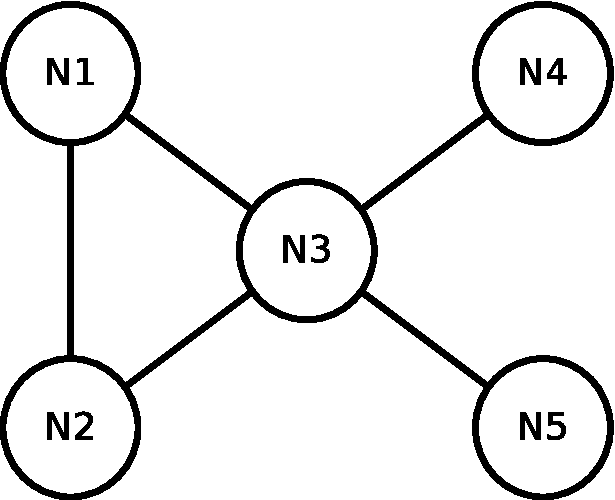
\includegraphics[width=0.45\columnwidth]{images/undirected-graphical-model-example}
\par\end{centering}
\caption[Example of an Undirected Graph.]{\label{fig:Example-of-an-Undirected-Graph}Example of an Undirected
Graph encoding the following conditional independencies: the node
pairs (N1,N4), (N1,N5), (N2,N4), (N2,N5),(N4,N5) are conditionally
independent given node N3. (But (N1,N2) are not conditionally independent
given N3.)}
\end{figure}

For example, if there are the three cliques $\mathbf{C_{1}}=\{N_{1},N_{2},N_{3}\}$,
$\mathbf{C_{2}}=\{N_{3},N_{4}\}$, and $\mathbf{C_{3}}=\{N_{3},N_{5}\}$
(see figure \ref{fig:Example-of-an-Undirected-Graph}), then the joint
probability distribution $P$ (also called \index{Gibbs distribution}Gibbs
distribution) can be written as: 
\[
P(N_{1},\dots,N_{5})=\frac{1}{Z}\phi_{1}(\mathbf{C_{1}})\phi_{2}(\mathbf{C_{2}})\phi_{3}(\mathbf{C_{3}}),
\]
where $\phi_{1}(\mathbf{C_{1}})=\phi(N_{1},N_{2},N_{3})$ is the potential
function of clique 1 (\emph{clique potential}\index{clique potential}),
and is a function of the 3 random variables $N_{1},N_{2},N_{3}$ in
the clique. $Z$ is the partition function and must normalize the
function so that $P$ is a probability: 
\[
Z=\sum_{X_{1},\dots,X_{n}}\phi_{1}(\mathbf{C_{1}})\phi_{2}(\mathbf{C_{2}})\phi_{3}(\mathbf{C_{3}}).
\]

In practice, $\phi_{1}(N_{1},N_{2},N_{3})$ can be represented by
a table that holds, for each possible combination of states of the
three random variables, a positive real number. For example, if each
of the three random variables has two states, then the table (with
$2^{3}$ entries) could look like in table \ref{tab:Example-of-potential-function}.

\begin{center}
\begin{table}
\begin{centering}
\begin{tabular}{|c|c|c||c|}
\hline 
$n_{1}$ & $n_{2}$ & $n_{3}$ & $\phi(N_{1}=n_{1},N_{2}=n_{2},N_{3}=n_{3})$\tabularnewline
\hline 
\hline 
A & A & A & 0.124\tabularnewline
\hline 
A & A & B & 2.553\tabularnewline
\hline 
A & B & A & 0.842\tabularnewline
\hline 
$\vdots$ & $\vdots$ & $\vdots$ & $\vdots$\tabularnewline
\hline 
B & B & B & 1.258\tabularnewline
\hline 
\end{tabular}
\par\end{centering}
\caption{\label{tab:Example-of-potential-function}Example of a potential function
$\phi$ represented as a table.}
\end{table}
\par\end{center}

\subsubsection{Directed Graphical Models}

\begin{figure}
\begin{centering}
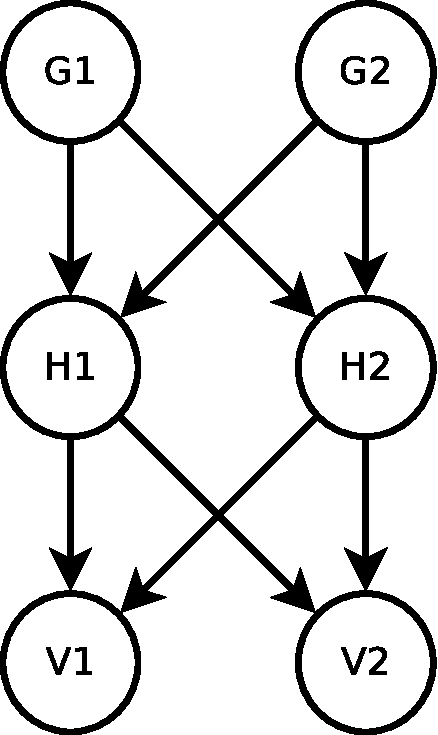
\includegraphics[width=0.3\columnwidth]{images/directed-graphical-model-example}
\par\end{centering}
\caption[Example of a Directed Graph.]{\label{fig:Example-of-a-Directed-Graph}Example of a Directed Graph.
Note that the graph is acyclic, and the nodes are laid out in layers.}
\end{figure}

Directed graphical models are also called \emph{Bayesian Networks}\index{Bayesian network}
or \emph{Belief Networks}\index{Belief network}. (See e.g. \cite{KollerTaskar2007,Neal1992}.)

Like undirected graphical models, directed graphical models represent
an implicit joint probability distribution over all random variables
present in the model. The graph must be directed and acyclic, and
each node of the graph is associated with a random variable. See figure
\ref{fig:Example-of-a-Directed-Graph} for an example.

A directed graphical model is defined by the directed graph $G=(\mathbf{N},\mathbf{E})$,
a prior probability distribution $P(N_{noparents})$ at the nodes
that do not have parents $\mathbf{N_{noparents}}$, and conditional
probability distributions $P(N_{hasparents}\mid\mathbf{N_{parents}})$
at the nodes that have parents $\mathbf{N_{hasparents}}$. In the
latter nodes the conditional probability distribution may only be
conditional on its immediate parents, not on distant ancestors. The
directed graph encodes the set of conditional independencies between
the random variables: A random variable $X$ of the graph is conditionally
independent of all random variables that are not descendants of $X$
(i.e. $\mathbf{N}\backslash\mathbf{N_{descendant(\mathbf{\mathrm{X}})}}$)
given the values of the parent variables of $X$ (this is called the
\emph{local Markov property}\index{local Markov property} of directed
graphs):
\[
X\,\,\indep\,\,(\mathbf{N}\backslash\mathbf{N_{descendant(\mathrm{X})}})\mid\mathbf{N_{parent(\mathrm{X})}}.
\]
(In general, independencies betweem any two sets of variables conditioned
on a third can be derived from the structure of the graph using \index{d-separation}\emph{d-separation}
\cite{Barber2012}.)

\paragraph{The Joint Probability Distribution Encoded by the Graphical Model\label{par:The-Joint-Encoded-by-Directed-Graphical-Model}}

In a directed graphical model, the random variables $\mathbf{N}$
can be totally ordered such that $N_{i}$ comes before $N_{j}$ if
there is a directed path from $N_{i}$ to $N_{j}$ in the graph, and
the order is unspecified if there is no directed path between $N_{i}$
and $N_{j}$ \cite{Neal1992}. (Thus, there are graphs which have
more than one compatible ordering, for example in the graph $A\rightarrow C\leftarrow B$,
the ordering can be $A,B,C$ as well as $B,A,C$.) In the following,
the ordering is expressed as the subscript $i\in\mathbb{N}$ of the
random variable $N_{i}$. The node $N_{i}$ has associated with it
the conditional probability $P(N_{i}=n_{i}\mid N_{j}=n_{j}\forall j<i)$.
(``The probability that the random variable $N_{i}$ is equal to
$n_{i}$ given that the random variables \textbf{$N_{j}$ }are equal
to $n_{j}$ where all subscripts $j$ that are smaller than $i$.'').

The joint probability distribution encoded by the graph is
\[
P(\mathbf{N})=P(N_{1}=n_{1},N_{2}=n_{2},\dots,N_{n}=n_{n})=\prod_{i=1}^{n}P(N_{i}=n_{i}\mid N_{j}=n_{j}\forall j<i).
\]

\paragraph{Example How to Represent the Conditional Probability Distribution}

For example, if the $N_{i}$ can only assume discrete $n_{i}$, the
conditional probability distribution can be represented by a table
with a size exponential in the number of involved nodes. When a node
has $a$ ancestors, each of which has $s$ possible states, and the
node itself also has $s$ possible states, then the table must contain
one probability for each of the $s^{a}\cdot(s-1)$ possible states.
($s^{a}$ for the combinations of the values of the ancestors and
$(s-1)$ for the values the node itself can assume.)

\subsection{Exact Inference in Graphical Models}

Inference in a graphical model is the task of answering a query about
the joint probability distribution encoded by the graph, or of a part
of the joint probability distribution. For example, one might be interested
in the overall probability of the configuration of a sub-set of variables.
However, in the general case this takes exponential time.

\subsubsection{Naive Approach: Marginalizing the Joint \label{par:Exact-Inference-in-Directed-and-Undirected Graphical Models}}

Since a graphical model is a representation of a joint probability
distribution, it can answer queries about probabilities of the joint
probability distribution encoded by the graphical model by first explicitly
calculating the joint, then marginalizing out non-interesting variables.

For example, we might want to infer the probability of a configuration
of variables when the values of only some of the variables are known.
We can then partition the variables $\mathbf{V}$ of a graphical model
into three disjoint groups:
\begin{enumerate}
\item the known variables $\mathbf{K}$,
\item the unknown variables $\mathbf{W}$ that we want to know the probability
distribution of,
\item the unknown variables $\mathbf{U}$ that we do not care about.
\end{enumerate}
Let the known values of $\mathbf{K}$ be written \textbf{$\mathbf{k}$}.
The unknown values of $\mathbf{W}$ are named \textbf{$\mathbf{w}$},
and the values of $\mathbf{U}$, $\mathbf{u}$. 

How to calculate the joint $P(\mathbf{W},\mathbf{U},\mathbf{K})$
encoded by the graphical model was defined in section \ref{par:The-Hammersley-Clifford-theorem-of-Undirected-Graphical-Model}
for undirected graphical models and in section \ref{par:The-Joint-Encoded-by-Directed-Graphical-Model}
for directed graphical models. Let's now turn our attention to marginalizing
out the non-interesting variables $\mathbf{U}$.

When we want to find the probability of configuration $\mathbf{W}=\mathbf{w}$,
given $\mathbf{K}=\mathbf{k}$, we can first write the query in terms
of the joint probability distribution. We have to condition on $\mathbf{K}$,
and marginalize out the unknown variables $\mathbf{U}$ that we do
not care about: 
\begin{eqnarray}
P(\mathbf{W}=\mathbf{w}|\mathbf{K}=\mathbf{k}) & = & \sum_{\mathbf{U}}P(\mathbf{W}=\mathbf{w},\mathbf{U}=\mathbf{u}|\mathbf{K}=\mathbf{k})\nonumber \\
 & = & \sum_{\mathbf{U}}\frac{P(\mathbf{W}=\mathbf{w},\mathbf{U}=\mathbf{u},\mathbf{K}=\mathbf{k})}{P(\mathbf{K}=\mathbf{k})}.\label{eq:Inference in graphical models}
\end{eqnarray}

In the above formula there is a sum over all variables \textbf{$\mathbf{U}$}.
Writing this out, we obtain 
\begin{eqnarray}
P(\mathbf{W}=\mathbf{w}|\mathbf{K}=\mathbf{k}) & = & \sum_{\mathbf{U}}\frac{P(\mathbf{W}=\mathbf{w},\mathbf{K}=\mathbf{k})}{P(\mathbf{K}=\mathbf{k})}\label{eq:Inference in graphical models, written out}\\
 & = & \sum_{U_{1}}\sum_{U_{2}}\cdots\sum_{U_{n}}\frac{P(\mathbf{W}=\mathbf{w},U_{1}=u_{1},U_{2}=u_{2},\dots,U_{n}=u_{n},\mathbf{K}=\mathbf{k})}{P(\mathbf{K}=\mathbf{k})}.\nonumber 
\end{eqnarray}

In the general case (if the joint probability cannot be factorized),
this nested sum needs $O(|\mathbf{u}|^{|\mathbf{U}|})=O(|\mathbf{u}|^{n})$
operations to compute, where $|\mathbf{u}|$ is the number of possible
values a variable $U_{i}$ can have (assuming for simplicity that
all random variables $U_{i}$ have the same number of possible values
$|\mathbf{u}|$) and $|\mathbf{U}|$ is the number of unknown variables
$U_{i}$. This is because all possible combinations of variable assignments
have to be considered. Thus, for this naive marginalization run-time
is exponential in the number of variables, and therefore intractable.

However, we have not yet considered the structure of the graph. We
can improve run-time in some cases of graphs and for some sets of
variables $\mathbf{K}$, $\mathbf{W}$, $\mathbf{U}$, as shown by
the following example.

\subsubsection{Factorization in Undirected Graphical Models}

In the case of an undirected graphical model, we can factorize the
joint probability into independent sub-joint-probabilities according
to the cliques. For instance, if the random variables $\mathbf{U}=\{U_{1},U_{2},\dots,U_{m}\}$
are composed of cliques $\mathbf{C_{1}},\mathbf{C_{2}},\dots,\mathbf{C_{n}}$,
so that $P(\mathbf{U})=\frac{1}{Z}\phi_{1}(\mathbf{C_{1}})\phi_{2}(\mathbf{C_{2}})\dots\phi_{n}(\mathbf{C_{n}})$,
then the above sum can be written, using Hammersley-Clifford, as
\begin{eqnarray*}
 & P(\mathbf{W}=\mathbf{w}|\mathbf{K}=\mathbf{k})\\
= & \sum_{U_{1}}\sum_{U_{2}}\cdots\sum_{U_{n}}\frac{P(\mathbf{W}=\mathbf{w},U_{1}=u_{1},U_{2}=u_{2},\dots,U_{n}=u_{n},\mathbf{K}=\mathbf{k})}{P(\mathbf{K}=\mathbf{k})}\\
= & \sum_{\mathbf{C}_{1}}\cdots\sum_{\mathbf{C}_{n}\backslash\{C_{1},\dots,C_{n-1}\}}\frac{\frac{1}{Z}\mbox{\ensuremath{\phi}}_{1}(\mathbf{W}=\mathbf{w},\mathbf{C}_{1}=\mathbf{c}_{1},\mathbf{K}=\mathbf{k})\cdot\ldots\cdot\mbox{\ensuremath{\phi}}_{n}(\mathbf{W}=\mathbf{w},\mathbf{C}_{n}=\mathbf{c}_{n},\mathbf{K}=\mathbf{k})}{P(\mathbf{K}=\mathbf{k})}\\
= & \frac{\frac{1}{Z}\left(\sum_{\mathbf{C}_{1}}\mbox{\ensuremath{\phi}}_{1}(\mathbf{W}=\mathbf{w},\mathbf{C}_{1}=\mathbf{c}_{1},\mathbf{K}=\mathbf{k})\cdot\left(\ldots\cdot\left(\sum_{\mathbf{C}_{n}\backslash\{C_{1},\dots,C_{n-1}\}}\mbox{\ensuremath{\phi}}_{n}(\mathbf{W}=\mathbf{w},\mathbf{C}_{n}=\mathbf{c}_{n},\mathbf{K}=\mathbf{k})\right)\right)\right)}{P(\mathbf{K}=\mathbf{k})}.
\end{eqnarray*}

The sums in the last line are nested sums that sum over all possible
states in the corresponding cluster. (If we order cliques descendingly
by the number of clique members then $\mathbf{C_{1}}$ is the largest
clique.) We still need to sum over the state combinations in the largest
clique. Therefore the run-time is at least $O(|\mathbf{u}|^{|\mathbf{C_{m}}|})$,
where $\mathbf{C_{m}}$ is the clique with the largest number of variables
in it. This is still an exponential run-time.


\subsubsection{Example of Inference in a Directed Graphical Model\label{subsec:Example-of-Exact-Inference-in-a-directed-graphical-model}}

Here we show an example how inference in a specific directed graphical
model is done. In our example, the directed graphical model is composed
of several densely connected layers, where the nodes within a layer
are not connected, and they have outgoing directed connections only
to nodes in the adjacent layer below.

When the probability distribution of the parent nodes are known, inferring
the probability distributions of child nodes is easy: just multiply
the probability of the parents with the conditional probability of
the child. To keep the example interesting, given the probability
distributions of the nodes in the bottom layer, we want to infer the
probability distributions for all the other nodes.

\paragraph{Deep Belief Networks}

For example consider the graph in figure \vref{fig:Example-of-a-Directed-Graph}.
This directed acyclic graph has the following directed connections
between its nodes: $G_{1}\rightarrow H_{1}$, $G_{1}\rightarrow H_{2}$,
$G_{2}\rightarrow H_{1}$, $G_{2}\rightarrow H_{2}$, $H_{1}\rightarrow V_{1}$,
$H_{1}\rightarrow V_{2}$, $H_{2}\rightarrow V_{1}$, $H_{2}\rightarrow V_{2}$.
Furthermore, the following conditional probability distributions are
given: $P(H_{1}|G_{1},G_{2})$, $P(H_{2}|G_{1},G_{2})$, $P(V_{1}|H_{1},H_{2})$,
$P(V_{2}|H_{1},H_{2})$. This layered architecture, where each node
in a layer is connected to all nodes in adjacent layers, defines a
directed graphical model called \emph{Deep Belief Network}\index{Deep Belief Network}.

\paragraph{Bayes Theorem Applied to Inference in a Deep Belief Network}

Now assume that $P(V_{1})$, $P(V_{2})$ are given and we want to
infer $P(G_{1}\mid\mathbf{V})$, $P(G_{2}\mid\mathbf{V})$, $P(H_{1}\mid\mathbf{V})$,
$P(H_{2}\mid\mathbf{V})$. Using Bayes' Theorem ($\mbox{posterior}=\mbox{likelihood}\cdot\mbox{prior}$)
we get
\begin{eqnarray}
P(H_{1},H_{2}|V,V_{2}) & = & \frac{P(V_{1},V_{2}|H_{1},H_{2})P(H_{1},H_{2})}{P(V_{1},V_{2})}\nonumber \\
 & = & \frac{P(V_{1},V_{2}|H_{1},H_{2})\left(\sum_{g_{1}}\sum_{g_{2}}P(g_{1})P(g_{2})P(H_{1}|g_{1},g_{2})P(H_{2}|g_{1},g_{2})\right)}{P(V_{1},V_{2})}\nonumber \\
 & = & \frac{1}{P(V_{1},V_{2})}\cdot P(V_{1}|H_{1},H_{2})P(V_{2}|H_{1},H_{2})\nonumber \\
 &  & \cdot\left(\sum_{g_{1}}\sum_{g_{2}}P(g_{1})P(g_{2})P(H_{1}|g_{1},g_{2})P(H_{2}|g_{1},g_{2})\right),\label{eq:deep-network-conditional-probability}
\end{eqnarray}
where 
\[
P(V_{1},V_{2})=\sum_{h_{1}}\sum_{h_{2}}P(V_{1}|H_{1}=h_{1},H_{2}=h_{2})P(V_{2}|H_{1}=h_{1},H_{2}=h_{2})P(H_{1}=h_{1},H_{2}=h_{2}).
\]
We can make the last transformation because $\ensuremath{V_{1}}$
and $\ensuremath{V_{2}}$ are independent given $\ensuremath{H_{1}},\ensuremath{H_{2}}$
(local Markov property). To determine $P(H_{1}|V_{1},V_{2})$ and
$P(H_{2}|V_{1},V_{2})$, we have to marginalize the other variable
in $\mathbf{H}$ out:
\begin{eqnarray}
P(H_{1}|V_{1},V_{2}) & = & \sum_{h_{2}}P(H_{1},H_{2}=h_{2}|V_{1},V_{2})\nonumber \\
P(H_{2}|V_{1},V_{2}) & = & \sum_{h_{1}}P(H_{1}=h_{1},H_{2}|V_{1},V_{2})\label{eq:deep-network-marginalization}
\end{eqnarray}

Since we now have $P(H_{1}|\mathbf{V})$, using $P(H_{1})=\sum_{v_{1}}\sum_{v_{2}}P(H_{1},V_{1}=v_{1},V_{2}=v_{2})$
and $P(H_{1}|V_{1},V_{2})=P(H_{1},V_{1},V_{2})/P(V_{1},V_{2})$ (and
equivalently $P(H_{1},V_{1},V_{2})=P(H_{1}|V_{1},V_{2})P(V_{1},V_{2})$),
we can determine $P(H_{1})$

\begin{eqnarray*}
P(H_{1}) & = & \sum_{v_{1}}\sum_{v_{2}}P(H_{1}|V_{1}=v_{1},V_{2}=v_{2})P(V_{1}=v_{1},V_{2}=v_{2}).
\end{eqnarray*}

$P(H_{2})$ can be computed similarly. Now that we know $P(H_{1})$
and $P(H_{2})$, we can repeat the steps to determine $P(G_{1}\mid\mathbf{H})$
and $P(G_{2}\mid\mathbf{H})$.

\subsubsection{Inference in Deep Belief Networks is Complicated\label{par:Exact-Inference-in-Deep-Belief-Networks-is-Complicated}}

The previous example shows that inference in a directed graphical
model with densely connected layers is complicated. If there are $n$
binary variables in $\mathbf{H}$ and $\mathbf{G}$, then the computation
of $P(\mathbf{H}\mid\mathbf{V})$ in equation \ref{eq:deep-network-marginalization}
takes $O(2^{n-1}n)$ due to having to marginalize out all variables
in $\mathbf{H}$ except one (the term $2^{n-1}$), and this for all
variables (the term $n$). In addition, this applies only if $P(\mathbf{H}\mid\mathbf{V})$
is known already. But in the computation of $P(\mathbf{H}\mid\mathbf{V})$,
equation \ref{eq:deep-network-conditional-probability}, there are
sums over the variables $g_{1}$ and $g_{2}$, which take another
$O(2^{n})$ in general. The phenomenon that leads to this computational
problem is called \emph{explaining away}\index{explaining away}.

The posterior of $H_{1}$ depends on all conditional probabilities
of the model, in this example, $P(\mathbf{V}\mid\mathbf{H})$ and
$P(\mathbf{H}\mid\mathbf{G})$. For Deep Belief Networks, which are
a kind of Directed Graphical Model with densely connected layers,
the conditional probabilities $P(\mathbf{V}\mid\mathbf{H})$ and $P(\mathbf{H}\mid\mathbf{G})$
have parameters called ``weights'' associated with them, and inference
of the layer immediately above $\mathbf{V}$, namely $\mathbf{H}$,
requires knowing all weights in the graph, not just those of $P(\mathbf{V}\mid\mathbf{H})$.
In addition, explaining away requires us to marginalize out all variables
in $\mathbf{H}$ except one, and this for all variables in $\mathbf{H}$.
A further problem is that we have to integrate over all variables
in all layers above $\mathbf{H}$ if we are interested in $P(\mathbf{H}\mid\mathbf{V})$.

These procedures become infeasible in a Belief Network with more than
a few parents per node. This is a problem in learning. If we want
to learn the parameters of a Deep Belief Network, we have to do inference.
However, we will see that there is a fast approximate learning algorithm.

\subsubsection{Intractability of Exact Inference on General Graphs}

Here we reference a proof by \cite{ChandrasekaranHarsha2012} that
low treewidth of the graph underlying inference in a graphical model
is the only structural property that enables tractable inference.

A \emph{triangulated graph}\index{triangulated graph} is a graph
where every loop having at least four nodes contains a \emph{chord}\index{chord},
i.e. an edge between two non-adjacent nodes in the loop\cite{Barber2012}.

For a triangulated graph, the \emph{treewidth}\index{treewidth} is
the number of nodes contained in the largest clique minus one. For
a graph of any form, the treewidth is the treewidth of the triangulation
that minimizes the treewidth. For directed acyclic graphs, the maximal
number of parents of any node is the critical number, since it determines
the treewidth of the moralized\footnote{You obtain a moralized graph from a directed acyclic graph by introducing
edges between all parents of a node, and then replacing directed edges
by undirected edges.} graph. (This was also shown by \cite{KwisthoutVanderGaag2010}.)

A graph is a \emph{minor}\index{minor of a graph}\emph{ }of a graph
$G$ if it is obtained from $G$ by one or more of the following operations:
1. deletion of an edge, 2. deletion of a node together with all edges
containing that node, and 3. contraction of an edge, which means an
edge $(N_{1},N_{2})$ and its two nodes $N_{1}$ and $N_{2}$ are
replaced with a new single node and the new node has edges to all
nodes that $N_{1}$ and $N_{2}$ had edges to.

Let $f(k)$ be the largest number such that every graph of treewidth
$k$ contains a grid of size $f(k)\times f(k)$ as minor. The \emph{grid-minor
hypothesis}\index{grid-minor hypothesis} states that $f(k)$ is polynomial
in $k$ (see \cite{ChandrasekaranHarsha2012}). \cite{ChekuriChuzhoy2014}
proved it in 2014.

A decision problem is in the complexity class $\mathbf{NP}$ if it
can be decided in time polynomial in the input by a non-deterministic
Turing machine. A decision problem is in the complexity class $\mathbf{P/Poly}$
if it can be decided in time polynomial in the input $x$ by a deterministic
Turing machine that receives as input not only $x$, but also an advice
string of length at most polynomial in the length of $x$ that may
only depend on the length of $x$, not $x$ itself\footnote{The advice string allows modeling pre-computation in the computation.}.
(See for example \cite{Sipser1996,Goldreich2008,AroraBarak2009}.)
The problem whether or not $\mathbf{NP}\subseteq\mathbf{P/Poly}$
is unsolved. 

\cite{ChandrasekaranHarsha2012} showed that under the assumptions
that the grid-minor hypothesis is true (which it is), and that $\mathbf{NP}\nsubseteq\mathbf{P/poly}$,
and given that arbitrary potential functions should be allowed, low
treewidth is the only structural property of otherwise arbitrary graphs
that ensures tractable run-time of exact inference on the graphical
model belonging to the graph. There exists no inference algorithm
with complexity polynomial in the treewidth.

If the assumption $\mathbf{NP}\nsubseteq\mathbf{P/poly}$ is correct,
then the only way to reduce the computational cost of exact inference
on a general graph with a given number of nodes is to reduce the
treewidth or to choose restricted potential functions (for example
constants) whose products do not require multiplication or can be
pre-computed. Therefore, in practice, the joint probability is approximated,
for example by Gibbs Sampling.

\subsection{Approximate Inference}

Approximate Inference in general graphical models by means of Gibbs
Sampling was first described by \cite{Neal1993}. We first have to
introduce Markov chains.

\subsubsection{Markov Chains}

For the following section, see e.g. \cite{Norris1997,GrinsteadSnell2003}
as references.


\paragraph{Markov property: Memorylessness}

A \emph{Markov chain}\index{Markov chain} is a sequence of random
variables $X_{t}$, where $t\in\mathbb{N}_{0}$ denotes the discrete
index of time. In a Markov chain, each random variable $X_{t}$ may
depend only on the state of the random variable at the immediate previous
time point $t-1$, i.e. 
\[
P(X_{t}=x_{t}\mid X_{0}=x_{0},\dots,X_{t-1}=x_{t-1})=P(X_{t}=x_{t}\mid X_{t-1}=x_{t-1})
\]
must hold for all $t\geq1$. This memorylessness is called the \emph{Markov
property}\index{Markov property}. In a Markov chain, possible states
$x_{t}$ at each time point are discrete and from the same set $\mathbb{S}$:
\begin{eqnarray*}
x_{t} & \in & \mathbb{S}\ \ \ \mbox{for all \ensuremath{t}}.
\end{eqnarray*}

\paragraph{Time-homogeneous Markov Chain and Transition Matrix}

A \emph{time-homogeneous Markov chain}\index{time-homogeneous Markov chain}
is a Markov chain in which the conditional probability $P(X_{t}=x_{t}|X_{t-1}=x_{t-1})$
is the same for all time points $t$, i.e. 
\[
P(X_{t}=x_{t}\mid X_{t-1}=x_{t-1})=P(X_{t-1}=x_{t-1}\mid X_{t-2}=x_{t-2})
\]
for all time points $t\geq2$. If this is the case, then this conditional
probability 
\[
P(X_{t}=j\mid X_{t-1}=i)\eqqcolon p_{ij}
\]
 is independent of the current time $t$ and can be written as the
matrix $p$, called the \emph{transition matrix}\index{transition matrix}.
In the following we will only deal with time-homogeneous Markov chains.

\paragraph{Computing future states from the initial distribution}

Let $d^{(t)}$ be the distribution of $X_{t}$, also named the \emph{probability
vector}\index{probability vector}, a row vector of length $|\mathbb{S}|$.
An entry $d_{i}^{(t)}$ is equal to the probability of $X_{t}$ having
state $x_{i}$: 
\begin{eqnarray*}
d_{i}^{(t)} & = & P(X_{t}=x_{i}).
\end{eqnarray*}
This implies $\sum_{i}d_{i}^{(t)}=1$ for all $t$. The distribution
$d^{(t+1)}$ can be computed from $d^{(t)}$ by matrix multiplication
with the transition matrix $p$: 
\[
d^{(t+1)}=d^{(t)}p.
\]
Given an initial distribution $d^{(0)}$ and the transition matrix
$p$, all $d^{(t)}$ are specified by 
\[
d^{(t)}=d^{(0)}p^{t}.
\]

\paragraph{Stationary distribution}

There are time-homogeneous Markov chains whose state distribution
stays constant once it has assumed a certain state distribution. Such
state distributions are called \emph{invariant}\index{invariant distribution}
or \emph{stationary distribution}\index{stationary distribution}.
A stationary distribution $\pi$ must fulfill the following equation:
\[
\pi p=\pi
\]
If $d^{(t)}=\pi$, then $d^{(t+u)}=\pi$ for all $u\geq0$. A Markov
chain can have more than one stationary distribution.

\paragraph{Detailed balance/Reversibility}

A Markov chain with transition matrix $p$ satisfies \emph{detailed
balance}\index{detailed balance}\emph{ }if there exists a probability
distribution $\pi=(\pi_{1},\pi_{2},\dots,\pi_{n})$ such that 
\[
\pi_{j}p_{ji}=\pi_{i}p_{ij}\ \ \ \mbox{for all \ensuremath{i}, \ensuremath{j}}.
\]
Such a Markov chain is also called a \emph{reversible} Markov chain\index{reversible Markov chain}
\cite{Norris1997}. A Markov chain with the detailed balance property
has at least one stationary distribution, where each stationary distribution
$\lambda$ fulfills the detailed balance condition: $\lambda_{j}p_{ji}=\lambda_{i}p_{ij}$
for all $i$, $j$.

While having detailed balance implies that a Markov chain has a stationary
distribution, the reverse is not true: there are Markov chains with
a stationary distribution but not satisfying detailed balance. For
example, a Markov chain with transition probabilities 
\[
(p_{ij})=\left(\begin{array}{ccc}
0 & 2/3 & 1/3\\
1/3 & 0 & 2/3\\
2/3 & 1/3 & 0
\end{array}\right)
\]
does not satisfy detailed balance, but $\pi=\left(\begin{array}{ccc}
\frac{1}{3} & \frac{1}{3} & \frac{1}{3}\end{array}\right)$ is a stationary distribution of this Markov chain \cite{Norris1997}.

\paragraph{Fundamental Theorem of Markov Chains\label{par:Fundamental-Theorem-of-Markov-Chains}}

Under what conditions does a Markov chain have an unique stationary
distribution? This is answered by the \emph{Fundamental Theorem of
Markov Chains}\index{fundamental theorem of Markov chains} \cite{Behrends2000}:

Theorem: Let $d^{(0)}$ and $e^{(0)}$ be any probability vectors
of a Markov chain with transition probabilities $(p_{ij})$, where
$(p_{ij})$ is irreducible, positive-recurrent and aperiodic. Then
the Markov chain converges to the unique stationary distribution $\pi$,
irrespective of the starting states:
\[
\lim_{t\rightarrow\infty}d^{(0)}p^{t}=\lim_{t\rightarrow\infty}e^{(0)}p^{t}=\pi.
\]

The definitions of irreducibility, positive recurrence, and aperiodicity
follow.

\paragraph{Irreducibility}

A Markov chain is called \emph{irreducible}\index{irreducible}, if
it is possible to go from any state $i$ of the Markov chain to any
state $j$ (possibly in more than 1 steps). Formally, a Markov chain
is called irreducible, if its states are all in the same (and only)
closed subset. A subset $C$ of $\mathbb{S}$ is called \emph{closed
}if $p_{ij}=0$ whenever $i\in C$ and $j\notin C$. (Remember that
$\mathbb{S}$ is the set of possible states of the Markov chain.)

\paragraph{Positive Recurrence}

A state $i$ of a Markov chain is \emph{positive recurrent}\index{positive recurrent},
if we expect the Markov chain to take a finite number of steps until
it is in state $i$ again, when it started in state $i$ at time point
$0$. To define positive recurrence formally, we have to define auxiliary
measures first. The probability that state $j$ is visited at time
step $k$ for the first time after the Markov chain had been in state
$i$ at time point $0$ is 
\[
f_{ij}^{(k)}:=P(X_{1}\neq j,X_{2}\neq j,\dots,X_{k-1}\neq j,X_{k}=j\mid X_{0}=i).
\]
The probability that state $j$ is ever reached from state $i$ is
\[
f_{ij}^{*}:=\sum_{k=1}^{\infty}f_{ij}^{(k)}.
\]
With this, we can define the expected number of steps for the Markov
chain to reach state $j$, when starting at state $i$:
\[
\mu_{ij}:=\sum_{k=1}^{\infty}kf_{ij}^{(k)}.
\]
This number is also called the \emph{mean recurrence time}\index{mean recurrence time}.
With these definitions, we can define a state to be \emph{transient}\index{transient},
positive recurrent, or \emph{null recurrent}\index{null recurrent}:
\begin{itemize}
\item If $f_{ii}^{*}<1$, the state $i$ is called transient.
\item If $f_{ii}^{*}=1$, the state $i$ is called recurrent.

\begin{itemize}
\item If $f_{ii}^{*}=1$ and $\mu_{ii}<\infty$, the state $i$ is called
\emph{positive recurrent}.
\item If $f_{ii}^{*}=1$ and $\mu_{ii}=\infty$, the state $i$ is called
\emph{null recurrent}.
\end{itemize}
\end{itemize}
It can be proven that when there are finitely many states, there are
no null recurrent states (see Proposition 7.2. in \cite{Behrends2000}).

\paragraph{Aperiodicity}

The definition of an \emph{aperiodic}\index{aperiodic} state is shorter.
The period of a state\index{period of a state} $i$ is defined as
the greatest common denominator of the number of time steps needed
for a Markov chain so that it is possible to be in state $i$ again,
after it was in state $i$ before: 
\[
period(i)=gcd(\{k\mid k\geq0,(p^{k})_{ii}>0\}).
\]
If $period(i)=1$, state $i$ is called \emph{aperiodic}. If all states
of a Markov chain are aperiodic, the Markov chain is called aperiodic.

\paragraph{Markov Chain Monte Carlo (MCMC)}

\emph{Markov Chain Monte Carlo}\index{Markov Chain Monte Carlo algorithm}\index{MCMC algorithm}
is an algorithm to sample from a multivariate probability distribution.
It sets up a Markov chain that converges to the desired stationary
distribution and iterates it through time until the stationary distribution
is approximated sufficiently.

A trick can be useful. To efficiently calculate the stationary distribution
$\pi$, compute only the transition matrix for time steps that are
a power of 2, i.e. $p^{2^{t}}$. This can be done by starting with
$p^{1}:=p$, repeated squaring: $p^{2t}:=p^{t}p^{t}$, and assigning
the stationary distribution $\pi=d^{(0)}p^{2^{t}}$ for a large enough
$t$.

MCMC will be described in the next section. 

\subsubsection{Gibbs Sampling}

Here, we will review Gibbs Sampling to show how \cite{Neal1993} used
it to approximate inference in directed and undirected graphical models.

\emph{Gibbs Sampling}\index{Gibbs sampling} \cite{GemanGeman1984}
is an instance of a Markov chain Monte Carlo (MCMC) algorithm. Its
goal is to generate samples from a multivariate joint probability
distribution, without having to know its closed form. The generated
samples can then be used to compute an approximation of the mean of
a distribution, for example.

To use a Gibbs Sampler, one must construct a Markov chain with its
(only) stationary distribution equal to the target distribution. Each
random variable is updated in turn, based on the conditional probabilities.

\paragraph{Gibbs Sampling Requires Closed-form Conditional Probabilities}

Suppose that the multivariate target distribution is $P(X_{1},\dots,X_{n})$.
Here, for each random variable $X_{i}\in\{X_{1},\dots,X_{n}\}$, the
conditional probability of the variable given all other variables
must be known in closed form, so that it can be evaluated: 
\[
P(X_{i}\mid\mathbf{X_{j}},j\in\{1,\dots,n\}\backslash i)=P(X_{i}\mid X_{1},\dots,X_{i-1},X_{i+1},X_{n}).
\]
Another prerequisite is that Gibbs Sampling, which requires sampling
from the conditional probability distribution and iterating, should
be faster than sampling from the joint target probability distribution
directly.

\paragraph{A Markov Chain in Multiple Dimensions}

The variable updates in Gibbs Sampling can be regarded as a Markov
chain. However, we must first define how the random variables of Gibbs
Sampling are mapped to the random variable of the Markov chain. One
possibility is to re-map the random variables and their states to
a single random variable.

Above, Markov chains were defined for a single state variable $X$.
But in Gibbs Sampling there are usually more than one variable, written
$X_{i}\in\{X_{1},\dots,X_{n}\}$ above. If there are a finite number
of random variables in Gibbs Sampling, and the state space of these
variables is also finite, say of size $m$, then the (therefore also
finite) number of states of these variables can be encoded in a single
variable with a state space of size $m^{n}$.

For example, say there are 3 variables, each of which can assume 2
states, and we want to encode these $2^{3}$ different possible states
in one variable. Then the Markov chain has one variable with $2*2*2$
different possible states.

\paragraph{Constructing a Markov Chain from Base Transitions}

\cite{Neal1993} suggests constructing a non-homogeneous Markov
chain with transition matrix $T$ by applying base transitions in
turn, each of which describe the probability of a state change of
one random variable. The base transitions are named $B_{k}(x,x')$,
where $k\in1,2,\ldots,s$ is the index of the base transition, $x$
is the starting state of the transition, $x'$ is the target state
of the transition. $B_{k}(x,x')$ is the probability of the transition
and must be strictly greater than zero for all values of $x$ and
$x'$, to make the Markov chain irreducible. At each time-point $a*s+k-1$
with $a\in\mathbf{\mathbb{N}}$, the next single base transition $B_{k}(x,x')$
is then applied:

\[
T_{as+k-1}(x,x')=B_{k}(x,x').
\]

\cite{Neal1993} also notes that the required properties for a Markov
chain to converge are fulfilled: If each of the base transitions $B_{k}$
have a stationary distribution, then the non-homogeneous $T$ also
has a stationary distribution.

\paragraph{Initialization of the Gibbs Sampler}

A Gibbs Sampler starts by specifying a start value $x_{i}^{(0)}$
for each random variable $X_{i}$. Since the Markov chain must be
constructed such that it converges to its only stationary distribution
the choice of start values is not critical, but it influences the
numbers of iterations needed until the Gibbs Sampler returns samples
from the target distribution. So the start value should be close to
the expected value of the distribution.

\paragraph{Iterating}

Then an iterative process is started. In each iteration $t$, each
random variable $X_{i}$ is updated by sampling a new value $x_{i}^{(t)}$
from the conditional probability distribution 
\begin{equation}
P(X_{i}\mid X_{1}=x_{1}^{(t-1)},\dots,X_{i-1}=x_{i-1}^{(t-1)},X_{i+1}=x_{i+1}^{(t-1)},\dots,X_{n}=x_{n}^{(t-1)}).\label{eq:Gibbs sampling: CPD}
\end{equation}

There are different alternative ways in which the random variables
are updated, for example updating the random variables can be done
in random order, or sequentially, or a whole ``block'' of multiple
random variables can be sampled from the conditional distribution
given all the other random variables (e.g. $P(X_{i_{1}},X_{i_{2}},X_{i_{3}}\mid\mathbf{X_{j}=x_{j}^{(t-1)}},j\in\{1,\dots,n\}\backslash\{i_{1},i_{2},i_{3}\})$).

If the Markov chain fulfills irreducibility, positive recurrence,
and aperiodicity, then it is guaranteed to converge to its stationary
distribution (Fundamental Theorem of Markov Chains). However there
is currently no known analytic method to determine when the Markov
chain has reached its stationary distribution, which leads to the
following two strategies, \emph{burn-in} and \emph{thinning}.

\paragraph{Burn-in Period}

The starting value of the random variable might be far from the ``center''
of the distribution. But after some number of throw-away iterations,
the Gibbs Sampler's values $\mathbf{x}=(x_{1},\dots,x_{n})$ will
start coming from the target joint distribution $P(X_{1},\dots,X_{n})$.
This ``some number of throw-away iterations'' is called the \emph{burn-in
period}\index{burn-in period} and can be considerable depending on
the starting values and the joint probability distribution underlying
the conditional probability distributions. If one knows where the
``center'' of the equilibrium distribution is then one should use
a value near that center as the starting point, however, in many cases
such things are not known (and may be the goal of Gibbs Sampling in
the first place).

There is no known analytic method to determine when a chain is burned-in.
Several convergence diagnostics methods have been proposed, see e.g.
\cite{CowlesCarlin1996} for a review.

\paragraph{Thinning}

\index{thinning}Even after the Markov chain is burned in, there is
still a problem with the returned samples, which prevent them from
being used in those applications needing \emph{independent }samples.
The samples of two adjacent time steps $\mathbf{x}^{(t)}$ and $\mathbf{x}^{(t+1)}$
are correlated however, because the latter is dependent on the former
(by definition).

This can be mitigated by returning only the states of every $n$th
iteration, where $n$ is a sufficiently large number. This is called
``thinning'' of the Gibbs sampler.

Again, there is currently no straightforward analytic way to determine
what a sufficiently large $n$ is for the adjacent $\mathbf{x}$ to
be regarded independent. In practice one resorts to heuristics like
autocorrelation.

\subsubsection{Gibbs Sampling in Markov Random Fields and Bayesian Networks \label{subsec:Inference-in-Markov-Random-Fields}}

We can now define the algorithms for approximate inference using Gibbs
Sampling in Markov Random Fields and Bayesian Networks.

In Markov Random Fields, we use the local Markov property: each random
variable $X_{i}$ is independent of all other random variables given
the states of the neighboring random variables. Thus, in Markov Random
Fields, the conditional probability (see equation \ref{eq:Gibbs sampling: CPD})
is 
\[
P(X_{i}\mid X_{1},\dots,X_{i-1},X_{i+1},\dots,X_{n})=P(X_{i}\mid\mathbf{X}_{Neighborhood(X_{i})}).
\]
In Bayesian Networks the conditional probability is 
\[
P(X_{i}\mid X_{1},\dots,X_{i-1},X_{i+1},\dots,X_{n})=P(X_{i}\mid\mathbf{X}_{MarkovBlanket(X_{i})}),
\]
where $\mathbf{X}_{MarkovBlanket(X_{i})}$ are the random variables
in the Markov Blanket of $X_{i}$.

\paragraph{Gibbs Sampling in Markov Random Fields\label{par:Gibbs-Sampling-in-Markov-Random-Fields}}

Exact inference in Markov Random Fields can be done by conditioning
on the known random variables and marginalizing out the uninteresting
variables (see section \ref{par:Exact-Inference-in-Directed-and-Undirected Graphical Models}).
The exponential runtime of exact inference can be circumvented by
approximate methods like Gibbs Sampling.

For example, we might want to infer the probability of a configuration
of variables when the values of only some of the variables are known.
We can partition the variables $\mathbf{X}:=\mathbf{U}\cup\mathbf{K}\cup\mathbf{W}$
of a graphical model into three disjoint groups:
\begin{enumerate}
\item the variables $\mathbf{K}$ whose states are known (for example because
they were measured)
\item the unknown variables $\mathbf{W}$ that we want to know the probability
distribution of,
\item the unknown variables $\mathbf{U}$ that we do not care about.
\end{enumerate}
Gibbs Sampling in Markov Random Fields uses a converging Markov chain
to sample from the target joint probability distribution. A prerequisite
is that the conditional probability distributions are known in closed
form.
\begin{enumerate}
\item Initialize the state $x_{i}^{(1)}$ of the random variable $X_{i}\in\mathbf{W}\cup\mathbf{U}$
with an arbitrary state.
\item Initialize the state $x_{i}^{(1)}$ of the known random variables
$X_{i}\in\mathbf{K}$ with their known state.
\item \label{enu:For-each-time}For each time point $t\in\{1,2,\dots\}$
do

\begin{enumerate}
\item Keep the known variables fixed (i.e. $x_{i}^{(t+1)}:=x_{i}^{(t)}$
for all $X_{i}\in\mathbf{K}$).
\item For each random variable $X_{i}\in\mathbf{W}\cup\mathbf{U}$ do

\begin{enumerate}
\item Given the states of all variables $\mathbf{X}\backslash X_{i}$, sample
a new $X_{i}$ from its conditional distribution $P(X_{i}=x_{i}^{(t+1)}\mid X_{1}=x_{1}^{(t)},\dots,X_{i-1}=x_{i-1}^{(t)},X_{i+1}=x_{i+1}^{(t)},\dots,X_{n}=x_{n}^{(t)})$.
The Hammersley-Clifford theorem  states that this conditional probability
is equal to $P(X_{i}=x_{i}^{(t+1)}\mid\mathbf{X}_{Neighborhood(X_{i})})$.
\end{enumerate}
\end{enumerate}
\item Repeat step \ref{enu:For-each-time} until the Markov chain converges.
\item Discard the states of the uninteresting random variables $\mathbf{U}$.
\item Return the states of the interesting random variables $\mathbf{W}$.
\end{enumerate}

\paragraph{Gibbs Sampling in Bayesian Networks}

We use the same algorithmic structure as for Markov Random Fields
above, but sample from a different conditional probability distribution
$P(X_{i}=x_{i}\mid\mathbf{X_{j}}=\mathbf{x_{j}}:j\neq i)$ when updating
the state of $X_{i}$ in step \ref{enu:For-each-time}(b).

The conditional probability of $X_{i}$ given all other nodes is equal
to its conditional probability given the values of the nodes in $X_{i}$'s
Markov Blanket $X_{MarkovBlanket(X_{i})}$
\[
P(X_{i}=x_{i}\mid\mathbf{X_{j}}=\mathbf{x_{j}}:j\neq i)=P(X_{i}=x_{i}\mid\mathbf{X}_{MarkovBlanket(X_{i})}=\mathbf{x}_{MarkovBlanket(X_{i})}),
\]
where $\mathbf{X}_{MarkovBlanket(X_{i})}$ is the set of $X_{i}$'s
parents and children, and its children's parents. Formally, and parallel
to section 4.1 in \cite{Neal1993}, the conditional probability distribution
$P(X_{i}=x_{i}\mid\mathbf{X}_{MarkovBlanket(X_{i})})$ is equal to
\begin{eqnarray*}
P(x_{i}\mid\{x_{i}:i\neq k\}) & = & P(x_{i}\mid\mathbf{x}_{MarkovBlanket(X_{i})})\\
 & = & \frac{P(x_{i}\mid\mathbf{x}_{Parent(i)})\prod_{j\in Child(i)}P(x_{j}\mid x_{i},\mathbf{x}_{Parent(j)\backslash i})}{\sum_{\tilde{x}_{i}}P(\tilde{x}_{i}\mid\mathbf{x}_{Parent(i)})\prod_{j\in Child(i)}P(x_{j}\mid\tilde{x}_{i},\mathbf{x}_{Parent(j)\backslash i})}.
\end{eqnarray*}

\section{Artificial Neural Networks}

Here we will introduce artificial neural networks that have been developed
as models of biological neural networks since in the middle of the
last century. The artificial neural networks introduced here are related
to Deep Belief Networks, namely Hopfield networks, Multilayer Perceptrons,
and (Restricted) Boltzmann Machines.

\paragraph{Distinction Between a Deterministic and Stochastic Network}

In a deterministic network\index{deterministic network} a node represents
a deterministic value. In contrast, in a stochastic network\index{stochastic network}
a node represents a probability distribution. If there is a set of
``output'' nodes, then in a deterministic setting the output can
be interpreted as a point in a high-dimensional space, while in a
stochastic network the output is the joint probability distribution
over all the random variables associated with the output nodes.

A stochastic network is more general than its deterministic counterpart,
since a stochastic network can be converted to a deterministic network,
but not vice-versa. This comes at a higher cost. Inference and learning
in stochastic networks take longer than in deterministic networks.

\paragraph{Distinction Between Feed-forward and Recurrent Networks}

A \emph{feed-forward network}\index{feed-forward neural network}\emph{
}is a network defined on a directed acyclic graph. In contrast, the
connections of a \emph{recurrent network}\index{recurrent neural network}\emph{
}may form cycles.

\subsection{Hopfield Networks}

\paragraph{Structure}

A \emph{Hopfield Network}\index{Hopfield Network} \cite{Hopfield1984}
is a deterministic recurrent network with $m$ nodes, each having
a binary state $n_{i}\in\{0,1\}$ for all nodes $i$. Every node is
connected with all others but not with itself. The connection from
node $N_{i}$ to node $N_{j}$ is directed and has a weight $w_{ij}\in\mathbb{R}$.
There is no self-connection from node $i$ to node $i$, and therefore
$w_{ii}=0$ for all nodes $i$. Hence, each node has $m-1$ outgoing
connections and $m-1$ incoming connections. There is also a real-valued
bias $b_{i}\in\mathbb{R}$ for each node $i$ that acts as a weight
of a connection from a ``virtual'' node that always has state 1.
Figure \ref{fig:Example-of-a-Hopfield-Network} shows an example of
the structure of a Hopfield Network.

\begin{figure}
\begin{centering}
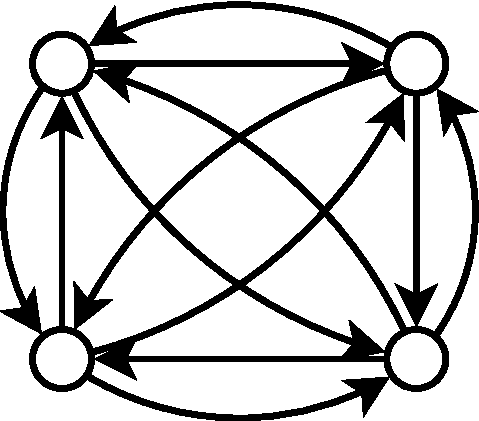
\includegraphics[width=0.3\columnwidth]{images/hopfield-network-example}
\par\end{centering}
\caption[Example of a Hopfield Network.]{\label{fig:Example-of-a-Hopfield-Network}Example of a Hopfield Network.
The circles are the nodes; the arrows are the (directed) connections.}
\end{figure}

\paragraph{Associative Memory}

Hopfield networks can be used as \emph{associative }or\emph{ content-addressable
memory}\index{associative memory}\index{content-addressable memory},
where the memory is a binary number. Bit $i$ of the memory is stored
in node $i$ of the network. Associative or content-addressable memory
means that the network can be initialized with a partially distorted
memory and the network can recall a previously learned memory that
is close to the initialized memory. Recalling a partially known memory
is done by repeatedly updating the network.

\paragraph{Updating Rule}

The network is updated asynchronously: At each time point $t$, a
node $i$ is chosen at random out of the $m$ possible nodes and it
is updated, while all other nodes remain constant. The state $n_{i}$
of node $i$ at time point $t$ is denoted $n_{i}^{(t)}$ and depends
on the state of all other nodes at time step $t-1$, the weights $w_{ji}$
from node $j$ to node $i$, and the bias $b_{i}$: 
\[
n_{i}^{(t)}=f\left(\sum_{j\neq i}n_{j}^{(t-1)}w_{ji}+b_{i}\right),
\]
where the \emph{activation function}\index{activation function} $f$
is a step function that maps nonpositive values to 0, and positive
values to 1: 
\[
f(x)=\begin{cases}
0 & \mbox{for }x\leq0\\
1 & \mbox{for }x>0
\end{cases}.
\]
(In \cite{Hopfield1984} there is also an external input to each
node, constant over all times $t$. Because the bias also does not
depend on $t$, both are combined into $b_{i}$ here.)\\
As described here, the updating rule is asynchronous (i.e. at each
time step a node is picked at random and its state is updated, which
is how Hopfield described it \cite{Hopfield1984}). Updating the
network synchronously (i.e. all nodes are updated at the same time)
is also possible.

\paragraph{Energy of a Hopfield Network}

The \emph{energy }\index{energy} is associated with the state of
the network at time point $t$ and is defined as

\begin{equation}
E^{(t)}=-\frac{1}{2}\sum_{i}\sum_{j\neq i}w_{ij}n_{i}^{(t)}n_{j}^{(t)}-\sum_{i}b_{i}n_{i}^{(t)}.\label{eq:Energy of a Hopfield network}
\end{equation}
Hopfield showed that when applying the updating rule repeatedly, the
energy converges to a (possibly local) minimum, provided that the
weights are symmetric (i.e. $w_{ij}=w_{ji}$) and there are no single-node
loops (i.e. $w_{ii}=0$). In more detail, each update of a node either
doesn't change the energy $E$ or decreases it. As time progresses
$E$ becomes smaller and smaller, i.e. $E^{(t)}\leq E^{(t-1)}$.


\paragraph{Recalling a Training Pattern by the Updating Rule}

Training a Hopfield network is the task of finding weights $w_{ij}$
and biases $b_{i}$, so that training patterns (i.e. memories to be
learned) have a low energy and all other states have a high energy.
After training, a Hopfield network can be initialized with a distorted
pattern, in which the states of some nodes are inverted. After iteratively
updating the network until its state doesn't change anymore, the stationary
state will be similar to a training pattern. In a demonstration of
\cite{Hopfield1982}, approximately 85\% of the trials ended in training
patterns, 5\% resulted in stable states near training patterns, and
10\% ended in stable states of no obvious meaning.

\subsection{Multilayer Perceptrons}

\paragraph{Structure}

A Multilayer Perceptron belongs to the class of deterministic feed-forward
neural networks. The neurons are arranged in layers, with the value
of nodes in a layer only depending on the values of nodes in the layer
above. Example structures of multilayer perceptrons were given in
figure \vref{fig:sigmoid-function} and figure \vref{fig:Data-flow-in-back-propagation}.

\subsubsection{Multilayer Feed-forward Networks as Universal Function Approximators}

\cite{HornikWhite1989} found that artificial feed-forward neural
networks with as few as one hidden layer can model any Borel measurable
function within a given error, provided the following conditions are
met:

\pagebreak{}
\begin{itemize}
\item The activation function must be a ``squashing'' function: A squashing
function $s(x)$ must be non-decreasing, $\lim_{x\rightarrow-\infty}s(x)=0$
and $\lim_{x\rightarrow\infty}s(x)=1$. An example is the sigmoid
function $\frac{1}{1+exp(-x)}$.
\item Sufficiently many hidden nodes must be available.
\end{itemize}
\cite{HornikWhite1989} also note that ``This {[}result{]} implies
that any lack of success in applications must arise from inadequate
learning, insufficient numbers of hidden units{[}nodes{]} or the lack
of a deterministic relationship between input and target.''

\subsubsection{Training Using Back-propagation}

\emph{Back-propagation}\index{back-propagation} is the adaptation
of weights and biases of the network to make its set of actual outputs
better fit a set of desired outputs for a given set of inputs. Technically
it is just running the network for a given input in the forward pass\index{forward pass},
observing the outputs in the output layer, computing the errors to
the desired outputs and back-propagating them to adapt the weights
and biases between all the layers. This will make the network output
values closer to the desired values next time this particular input
pattern is given to the network. The back-propagation algorithm is
a supervised learning step and thus prone to overfitting. In order
to discuss modifications and extensions of the algorithm, we will
first repeat the most important points of back-propagation as reviewed
in section \ref{subsec:Back-propagation}.

\paragraph{Forward and Backward Pass}

In the \emph{forward pass}\index{forward pass}, each node's output
is computed from the sum of its inputs
\begin{eqnarray*}
v_{j} & = & b_{j}+\sum_{i\in\mathbf{c_{j}}}o_{i}w_{ji},
\end{eqnarray*}
 where $b_{j}$ is the bias, $o_{i}$ is the output of a node in the
layer above, and $w_{ji}$ is the weight of the connection from node
$i$ to node $j$. The input $v_{j}$ is then scaled by the sigmoid
function to produce a node's output $o_{j}$

\[
o_{j}=\sigma(v_{j})=\frac{1}{1+\exp(-v_{j})}.
\]

In the \emph{backward pass}\index{backward pass}, the training procedure
computes the total error $E$ of the network, which is defined as
the squared sum of differences between actual output $o_{k}$ and
desired output $y_{k}$
\[
E=\frac{1}{2}\sum_{k}(o_{k}-y_{k})^{2},
\]
 where $o_{k}$ is the actual activation of node $k$ in the output
layer, and $y_{k}$ is its desired output. The sum-of-squared-differences
term $\frac{1}{2}\sum_{k}(o_{k}-y_{k})^{2}$ is called the \emph{error}\index{error function},\emph{
loss }\index{loss function}, or \emph{cost} function\index{cost function}.

\paragraph{Error of the Output Layer}

The error is then differentiated with respect to a weight $w_{kj}$
for a connection from node  $j$ in the last hidden layer to node
$k$ in the output layer 
\begin{equation}
\frac{\partial E}{\partial w_{kj}}=\frac{\partial E}{\partial o_{k}}\cdot\frac{\partial o_{k}}{\partial v_{k}}\cdot\frac{\partial v_{k}}{\partial w_{kj}}=(o_{k}-y_{k})\cdot o_{k}(1-o_{k})\cdot o_{j},\label{eq:backpropagation-error-wrt-weight}
\end{equation}
 and with respect to $b_{k}$
\[
\frac{\partial E}{\partial b_{k}}=\frac{\partial E}{\partial o_{k}}\cdot\frac{\partial o_{k}}{\partial v_{k}}\cdot\frac{\partial v_{k}}{\partial b_{k}}=(o_{k}-y_{k})\cdot o_{k}(1-o_{k})\cdot1.
\]

\paragraph{Error of the Other Layers}

The derivative of the error with respect to the weights $w_{ji}$
of the remaining connections from node $i$ in a layer to node $j$
in the layer below is
\begin{eqnarray*}
\frac{\partial E}{\partial w_{ji}} & = & \frac{\partial E}{\partial o_{j}}\cdot\frac{\partial o_{j}}{\partial v_{i}}\cdot\frac{\partial v_{i}}{\partial w_{ji}}\\
 & = & \frac{\partial E}{\partial o_{j}}\cdot o_{j}(1-o_{j})\cdot o_{i},
\end{eqnarray*}
 where
\begin{eqnarray*}
\frac{\partial E}{\partial o_{j}} & = & \sum_{k}\frac{\partial E}{\partial o_{k}}\frac{\partial o_{k}}{\partial v_{k}}w_{kj}
\end{eqnarray*}
and we take the value for $\frac{\partial E}{\partial o_{k}}\frac{\partial o_{k}}{\partial v_{k}}$
from node $k$, which is in the layer below node $j$. Analogously,
the derivative with respect to $b_{j}$ is 
\begin{eqnarray*}
\frac{\partial E}{\partial b_{j}} & = & \sum_{k}\frac{\partial E_{k}}{\partial o_{k}}\frac{\partial o_{k}}{\partial v_{k}}w_{kj}\cdot o_{j}(1-o_{j})\cdot1.
\end{eqnarray*}

\paragraph{Updating Rule and Learning Rate}

After computing the derivatives of the error with respect to the parameters
of the network, we can perform gradient descent and update the parameters
using the learning rate\index{learning rate} $\epsilon$, a small
positive number:
\begin{eqnarray}
\Delta w & = & -\epsilon\frac{\partial E}{\partial w}\label{eq:backpropagation-deltas}\\
\Delta b & = & -\epsilon\frac{\partial E}{\partial b}.\nonumber 
\end{eqnarray}

\paragraph{Optimizing the Sum of Squared Differences Error\label{par:Optimizing-the-Sum-of-Squared-DIfferences}}

Usually in back-propagation, the error function to be minimized is
the \emph{sum of squared differences}\index{sum of squared errors}\index{squared-error sum}
between the desired outputs and the actual outputs
\[
E=\frac{1}{2}\sum_{k}(o_{k}-y_{k})^{2},
\]
 where $y_{k}$ is the desired value of node $k$ in the output layer
and $o_{k}$ is the actual output value of node $i$. As stated in
equation \ref{eq:backpropagation-error-wrt-weight}, the derivative
of the error $E$ with respect to a weight $w_{kj}$ is
\begin{equation}
\frac{\partial E}{\partial w_{kj}}=(o_{k}-y_{k})\cdot o_{k}(1-o_{k})\cdot o_{j}.\label{eq:backpropagation-error-wrt-weight-1}
\end{equation}

\paragraph{Optimizing the Cross-entropy Error\label{par:Optimizing-the-Cross-entropy-error}}

Another error function is the \emph{cross-entropy error}\index{cross-entropy error}
\cite{NasrJoun2002} 
\[
E=-\sum_{k}y_{k}\log o_{k}-\sum_{k}(1-y_{k})\log(1-o_{k}),
\]
 where again $y_{k}$ is the desired output value of node $k$ in
the output layer and $o_{k}$ is the actual output value. The derivative
of error $E$ with respect to a weight $w_{kj}$ from node $j$ in
the last hidden layer to node $k$ in the output layer is then
\[
\frac{\partial E}{\partial w_{kj}}=(o_{k}-y_{k})o_{j}.
\]

\cite{GolikNey2013} note that using the cross-entropy error function
requires less updates, since the gradient for the sum-of-squared-differences
error function becomes low not only when the actual output $o_{k}$
is near the desired output $y_{k}$, but also when $o_{k}$ is near
0 or 1 (see equation \ref{eq:backpropagation-error-wrt-weight-1}).

\subsubsection{Parameters in Training a Neural Network\label{subsec:Parameters-of-Training-a-Multilayer-Perceptron}}

Although described here for multilayer perceptrons, the parameters
apply to most artificial neural networks, not just multilayer perceptrons.

\paragraph{Random Weight and Bias Initialization}

At the start of training, weights $w$ and biases $b$ have to be
initialized. They must not all be initialized to the same value, because
then the activations in the output layer $o_{k}$ would become equal,
leading to an equal error gradient for the weights and biases, which
would prevent learning. Ideally, the hidden and output layer activations
$o_{j}$ should be in the linear region of the activation function,
so that the error derivatives are large. As \cite{LeCunMuller1998}
note, this requires coordinating the training set  normalization,
the choice of the activation function, and the weight and bias initialization.

Usually the biases are initialized to zero, and the weights are drawn
from a uniform random distribution in {[}-1;1{]}, or from a normal
distribution with mean 0 and standard deviation 1. Another possibility
is to use ``fan-in'' initialization, where the number of incoming
connections $m$ to a node are taken into account. Then the weights
are randomly drawn from a normal distribution with mean 0 and standard
deviation
\[
\sigma=m^{-1/2}.
\]

\paragraph{Activation Function\label{The-sigmoid-activation-function}}

The activation of hidden and visible nodes are a function of the sum
of their inputs. The function that maps the sum of the inputs of a
node to its value is called the \emph{activation function}\index{activation function}.

The sigmoid activation function
\[
\sigma(x)=\frac{1}{1+e^{-x}}
\]
 is a standard activation function, often used in neural networks.
It is almost linear for inputs around zero, tends to 1 as its inputs
go to positive infinity and to 0 as inputs go to negative infinity
(see figure \vref{fig:sigmoid-function}).

Another commonly used activation function is the hyperbolic tangent
function 
\[
tanh(x)=\frac{1-e^{-2x}}{1+e^{-2x}}.
\]
Its graph looks very similar to the graph of the sigmoid function.
While the output range of the sigmoid is $[0;1]$, it is $[-1;1]$
for the hyperbolic tangent function.

In this work only the sigmoid activation function was used.

\paragraph{Momentum of the Learning Rule\label{par:Momentum-of-the-learning-rule}}

Usually, the learning rule includes a \emph{momentum}\index{momentum}
term. In this case, the weight and bias deltas from equation \ref{eq:backpropagation-deltas}
are replaced with a momentum weight delta $\Delta w_{momentum}$ and
momentum bias delta $\Delta b_{momentum}$. The momentum term 
\begin{eqnarray*}
\Delta w_{momentum}^{(t)} & = & \mu\Delta w_{momentum}^{(t-1)}+(1-\mu)\Delta w^{(t)}\\
\Delta b_{momentum}^{(t)} & = & \mu\Delta b_{momentum}^{(t-1)}+(1-\mu)\Delta b^{(t)},
\end{eqnarray*}
 includes a coefficient $\mu$ that is the fraction of the weight
and bias deltas of the previous time step $t-1$ to be added to the
current weight deltas where $\Delta w^{(t)}$ and $\Delta b^{(t)}$
are taken from equation \ref{eq:backpropagation-deltas}.

Momentum works like a low-pass filter and reduces oscillations during
learning by smoothing the weight and bias deltas added to the parameters
of the network. However, too large a momentum coefficient can cause
``explosion'', or non-convergence of the model during training.
To prevent this, $\mu$ is usually gradually increased to its final
value during the early steps of training.

The coefficient $\mu$ is an additional meta-parameter in training.

\subsubsection{Difficulties in Training Multi-layer Neural Networks}

Training a randomly initialized feed-forward neural network with more
than one hidden layer using back-propagation is difficult and usually
does not succeed. When attempting to train such a network, each node
in the output layer often just outputs the mean value of the desired
output of the training cases, independently of the input. One problem
is that there are many local minima (generated by repeatedly adding
weighted sigmoid functions) in the implicitly optimized energy function
during back-propagation \cite{GoriTesi1992}. Another problem is that
in discriminative learning, each training case only contributes as
many bits to the specification of the network parameters as needed
to specify the label \cite{Hinton2010}.

\subsection{Regularizations of Neural Networks}

Several regularization\index{regularization} methods for neural networks
have been developed over the years. They have in common that they
artificially constrain the search space of weights and biases in order
to let the model find better error minima or to prevent overfitting.
The neural network should do less ``learning by heart'' and instead
make its predictions apply to more unseen test set data.

The regularizations described here apply to most artificial neural
networks, not just multilayer perceptrons.

\subsubsection{L1 and L2 Weight Decay\label{subsec:L1-and-L2-Weight-Decay}}

L1 and L2 weight decay\index{L1 weight decay}\index{L2 weight decay}
penalize large weights by moving them towards zero. Both weight decay
methods decrease the absolute value of each weight in each training
iteration, in order to prevent large weights. This can be necessary
because for some training samples, some weights tend to ``escape'',
i.e. become larger and larger in absolute value, making subsequent
changes to the weights more difficult.

Instead of the normal weight delta $\Delta w$ defined in equation
\ref{eq:backpropagation-deltas}, L1 weight decay uses a penalized
weight delta 
\begin{eqnarray*}
\Delta w_{L1} & = & \Delta w-c*sgn(w),
\end{eqnarray*}
 where $c\in\mathbb{R}^{+}$ is a small positive constant meta-parameter,
the ``weight-cost'' of L1 weight decay, and $sgn(w)$ is the sign
of the weight, i.e. -1, 0, 1, for the weight $w$ being negative,
zero, positive, respectively.

L2 weight decay uses
\[
\Delta w_{L2}=\Delta w-w*c,
\]
 where $c\in\mathbb{R}^{+}$ is the small positive ``weight-cost''
of L2 weight decay.

\cite{Hinton2010} notes that there are four different reasons for
using weight decay: better generalization of the resulting network,
making the weights more interpretable by shrinking large weights,
penalize network nodes that are always firmly on or off due to large
inputs caused by large weights, and improve the mixing rate of contrastive
divergence\footnote{Contrastive divergence is explained in section \ref{subsec:Training-Restricted-Boltzmann-Machines-using-Contrastive-Divergence}.},
a training procedure for Restricted Boltzmann Machines, where small
weights increase the mixing rate of the Gibbs chain.

As \cite{FischerIgel2012} note, using an L2 weight decay term in
the updating term corresponds to assuming a zero-mean Gaussian prior
on the parameters in a Bayesian framework.

\subsubsection{Sparsity\label{subsec:Sparsity-Target}}

Sparsity regularization is a method to make only a small fraction
of hidden nodes output an activation very different from zero. Sparse
activity helps in the network's ability to generalize, and also makes
the trained network more interpretable \cite{Ng2011,Hinton2010,NairHinton2009}.
Like other regularization methods, sparsity regularization constrains
the space of possible parameters of the model.

\paragraph{Average Activation}

We first have to define what we mean by sparse activity. We can define
an \emph{average activation} $q_{j}$ of each hidden node $j$, and
encourage the node to have an average activation $q_{j}$ close to
a \emph{sparsity target}\index{sparsity target} $0<p\ll1$. We want
to approximately enforce that $q_{j}\approx p$. 

One way to define the average activation $q_{j}$ of node $j$ is
to take into account the node's activations in the previous training
iterations. The average activation $q_{j}$ can be defined to be an
exponentially decaying average of the activation $o_{j}^{(t)}$
\[
q_{j}^{(t)}=\lambda q_{j}^{(t-1)}+(1-\lambda)o_{j}^{(t)},
\]
 where $\lambda\in(0;1)$ is the \emph{decay rate}\index{decay rate (sparsity)},
$o_{j}^{(t)}$ is the activation of node $j$ at training iteration
$t$, and $q_{j}^{(t)}$ is its average activation at training iteration
t.

Alternatively, we can measure the average activation $q_{j}$ within
one training iteration, by defining $q_{j}$ as the average activation
over all $m$ training samples
\[
q_{j}=\frac{1}{m}\sum_{s}^{m}o_{j}^{(s)},
\]
 where $o_{j}^{(s)}$ is the activation of hidden node $j$ when the
input layer of the network has been set to training sample $s$.

\paragraph{Sparsity Error Term}

The idea is to add to the error term $\frac{\partial E}{\partial o_{j}}$
of a hidden node $j$ an additional term that encourages the node
to have an average activation $q_{j}$ close to the sparsity target
$p$. The term should be small when the average activation $q_{j}$
is close to the sparsity target $p$ and become larger when it deviates.
One such term is the Kullback-Leibler divergence between a Bernoulli
random variable with mean $p$ and a Bernoulli random variable with
mean $q_{j}$
\begin{eqnarray*}
E_{sparsity} & = & D_{KL}(P_{Bernoulli(p)}||P_{Bernoulli(q_{j})})\\
 & = & p\log\frac{p}{q_{j}}+(1-p)\log\frac{1-p}{1-q_{j}}.
\end{eqnarray*}
It is zero for $q_{j}=p$, and approaches infinity when $q_{j}=0$
or $q_{j}=1$. Differentiating this sparsity error with respect to
the weight $w_{ji}$ of a connection from node $i$ to node $j$,
and approximating the average activation $q_{j}$ to be equal to the
activation $o_{j}$ gives
\begin{eqnarray*}
\frac{\partial E_{sparsity}}{\partial w_{ji}} & = & \frac{\partial E_{sparsity}}{\partial o_{j}}\cdot\frac{\partial o_{j}}{\partial v_{j}}\cdot\frac{\partial v_{j}}{\partial w_{ji}}\\
 & \approx & \left(\frac{\partial}{\partial o_{j}}p\log\frac{p}{o_{j}}+(1-p)\log\frac{1-p}{1-o_{j}}\right)\cdot\frac{\partial o_{j}}{\partial v_{j}}\cdot\frac{\partial v_{j}}{\partial w_{ji}}\\
 & = & \left(\frac{1-p}{1-o_{j}}-\frac{p}{o_{j}}\right)\cdot\frac{\partial o_{j}}{\partial v_{j}}\cdot\frac{\partial v_{j}}{\partial w_{ji}}\\
 & = & \left(\frac{1-p}{1-o_{j}}-\frac{p}{o_{j}}\right)\cdot o_{j}(1-o_{j})\cdot o_{i}\\
 & = & (o_{j}-p)\cdot o_{i}.
\end{eqnarray*}
Substituting $q_{j}$ back for $o_{j}$ gives
\[
\frac{\partial E_{sparsity}}{\partial w_{ji}}\approx(q_{j}-p)\cdot o_{i}.
\]
Analogously, the derivative of the sparsity error with respect to
the bias $b_{j}$ of node $j$ is 
\begin{eqnarray*}
\frac{\partial E_{sparsity}}{\partial b_{j}} & = & \frac{\partial E_{sparsity}}{\partial o_{j}}\cdot\frac{\partial o_{j}}{\partial v_{j}}\cdot\frac{\partial v_{j}}{\partial w_{ji}}\\
 & \approx & (q_{j}-p)\cdot1.
\end{eqnarray*}

\paragraph{Complete Updating Rule}

For a training iteration, both the bias $b_{j}$ of node $j$ and
its incoming weights $w_{ji}$ must be adjusted by the derivative
of the sparsity error, scaled by the sparsity cost\index{sparsity cost}
$\lambda$
\begin{eqnarray*}
\Delta w_{ji} & = & -\epsilon\left(\frac{\partial E}{\partial w_{ji}}+\lambda\frac{\partial E_{sparsity}}{\partial w_{ji}}\right)\approx-\epsilon\left(\left(\sum_{k}\frac{\partial E}{\partial o_{k}}\frac{\partial o_{k}}{\partial v_{k}}w_{kj}o_{j}(1-o_{j})\right)+\lambda(q_{j}-p)\right)o_{i}\\
\Delta b_{j} & = & -\epsilon\left(\frac{\partial E}{\partial b_{j}}+\lambda\frac{\partial E_{sparsity}}{\partial w_{ji}}\right)\approx-\epsilon\left(\left(\sum_{k}\frac{\partial E}{\partial o_{k}}\frac{\partial o_{k}}{\partial v_{k}}w_{kj}o_{j}(1-o_{j})\right)+\lambda(q_{j}-p)\right).
\end{eqnarray*}

\subsubsection{Dropout\label{subsec:Dropout}}

Dropout\index{dropout} is a regularization method to make the nodes
in the hidden layers, which can be seen as feature detectors, less
dependent on each other \cite{SrivastavaSalakhutdinov2014}. This
is enforced by ``dropping'' during each training iteration a random
subset of nodes in a hidden or visible layer. This prevents subsequent
layers from adapting to specific combinations of node activations
in the previous layer, in which nodes are only useful in the context
of a large number of other nodes. It thereby reduces overfitting.
Dropout can be used in any neural network whose input to a node is
computed from several input nodes. 

Dropout specifies a probability $d$ for nodes in a layer with $n$
nodes to be active during a training iteration. In each iteration,
on average only $d*n$ nodes' output values $o_{j}$ are computed
and the other nodes are set to contribute nothing (i.e. $o_{j}:=0$)
to the input to the next layer. To utilize all trained nodes during
testing, all nodes contribute to the computation of input to a layer,
but their total input must then be multiplied by $d$, to simulate
that only a fraction of $d$ nodes are active.

The reasoning behind dropout is that for a network with $n$ nodes,
there are $2^{n}$ possible ways to drop out those nodes. During testing,
a network trained with dropout implicitly averages its output over
all these $2^{n}$ networks. This is faster than to do explicit model
averaging over $2^{n}$ networks with shared weights.

Dropping out a random fraction of nodes prevents single nodes from
co-adapting to the specific workings of a large number of other nodes.
\cite{SrivastavaSalakhutdinov2014} note that a side-effect of dropout
is that the activations of nodes become sparse, without another sparsity-inducing
regularization method being used.


\subsubsection{Early Stopping\label{subsec:Early-stopping}}

Early stopping\index{early stopping} is not a regularization method,
but still a method to prevent overfitting in supervised training of
an artificial neural network. The training data set is split into
a training data set and a validation data set, and uses only the training
data set for adapting the weights and biases during learning. After
each learning iteration, the validation data set is used to compute
the output error of the current network. After a defined number of
training iterations, the neural network that had the lowest output
error on the validation data set is used for predictions.

This prevents the training procedure from overfitting to sampling
error present in the training data set \cite{Prechelt1997}.

\subsection{Autoencoder}

An algorithm that can train an artificial neural network deterministically
with more than one hidden layer is the \emph{auto-associator}\index{auto-associator},
or \emph{autoencoder}\index{autoencoder} \cite{BengioLarochelle2007}.
The algorithm is unsupervised and iteratively constructs deeper and
deeper networks. Its essential idea is the construction of an encoder
network and its anti-symmetric counterpart, the decoder network. Both
are trained using back-propagation, wherein the target output to be
achieved in the output layer is the same unsupervised training sample
as presented to the network in the input layer, hence the name of
the algorithm.

\begin{figure}
\begin{centering}
\hfill{}A 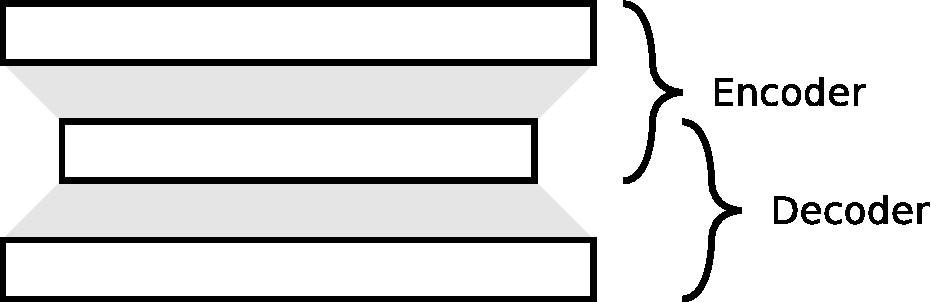
\includegraphics[width=0.4\columnwidth]{images/autoencoder-1}\hfill{}B
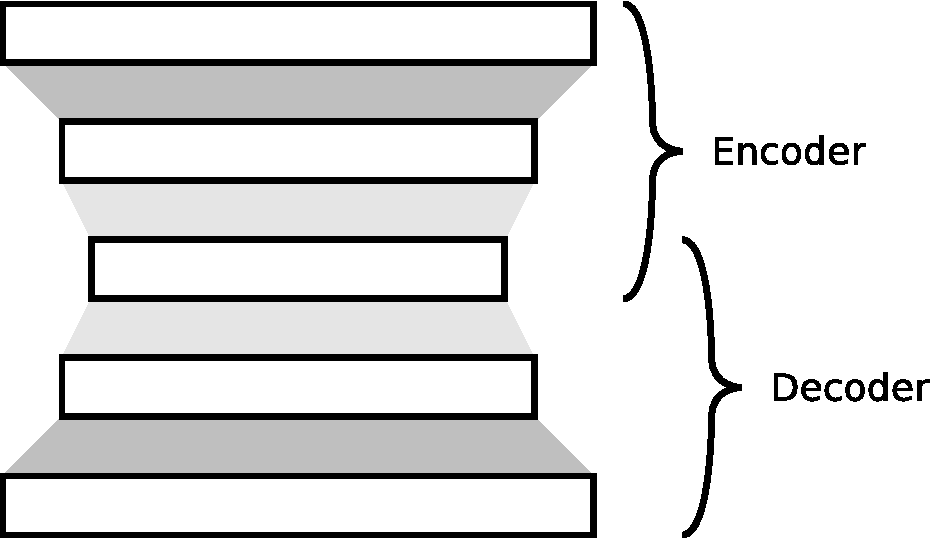
\includegraphics[width=0.4\columnwidth]{images/autoencoder-2}\hfill{}
\par\end{centering}
\caption[Training of an autoencoder.]{\label{fig:Training-of-an-autoencoder}Training of an autoencoder
iteratively adds hidden layers. The layers are depicted as rectangles.
 A: It starts with a network architecture of an input layer, one
hidden layer, and an output layer with the same size as the input
layer. The parameters of this small network are initialized randomly
(light gray area) and the network is trained. B: The hidden layer
is copied and another hidden layer is inserted between encoder and
decoder. The added weights are initialized randomly (light gray area),
and the whole network (\emph{including }the previously trained weights,
dark gray area) is trained. This procedure continues until the network
has enough layers.}
\end{figure}

The \emph{encoder}\index{encoder} starts in the first iteration as
a network that consists of the input layer and one hidden layer on
top. The (overlapping) \emph{decoder\index{decoder}} network consists
of the very same hidden layer and the output layer on top, which must
have the same dimensions as the input layer. Training an autoencoder
slowly adds internal layers to en- and decoder, see figure \ref{fig:Training-of-an-autoencoder}.
The network starts with three layers: input, hidden, and output layer.
This network is trained using back-propagation. Once back-propagation
does not improve the reconstruction error on the test set anymore,
the second step starts. In the second step, both encoder and decoder
are extended by one layer. The existing middle hidden layer is copied
and a new hidden layer is inserted in the middle. The new weights
are initialized randomly, for example by drawing from a uniform {[}-1;1{]}
distribution or from a normal distribution with mean 0 and standard
deviation 1, and the new biases are initialized to zero. Then back-propagation
is used again to determine the parameters of the whole network. This
process can be repeated until a sufficient number of hidden layers
has been trained.

Network size increases iteratively from 3 layers, to 5 layers, to
7 layers, and so on, and only 2 weight layers are initialized randomly
in each iteration. Therefore, the deep network is not stuck in a poor
local optimum, because there are only few new added weights each iteration,
and back-propagation finds parameters for a good (local) optimum.

The goal of training is that the network reconstructs as output patterns
the input patterns. One might think that that is too easy, since the
network could just learn the identity function at every layer, but
usually the number of nodes in at least one hidden layer is chosen
to be smaller than the number of nodes in the input (and output) layer.
In this way the autoencoder is forced to reconstruct its input from
a compressed representation. Another way to obtain interesting features
in the middle hidden layer is to use a regularization method on the
network.

\subsubsection{Encoder with a Classifier on Top}

The autoencoder as described is an unsupervised algorithm, because
it only reconstructs its input. The autoencoder can however be used
in a supervised fashion by first training its encoder and decoder
networks up to sufficient depth, and then removing the decoder network
and replacing it by a single output layer that has the dimension of
the training label. The weights between the last hidden layer of the
encoder and the new output layer as well as the biases of the new
output layer are initialized randomly (by drawing from a uniform or
normal distribution), and trained using back-propagation.

An encoder network trained using an autoencoder is a generative model\index{generative model},
because it was trained with the goal to reconstruct its input, and
the encoder's last hidden layer contains a compressed representation
of the input. Hence, an encoder with a classifier on top is a generative
model with a discriminative part put on top.

\subsection{Boltzmann Machines}

\begin{figure}
\begin{centering}
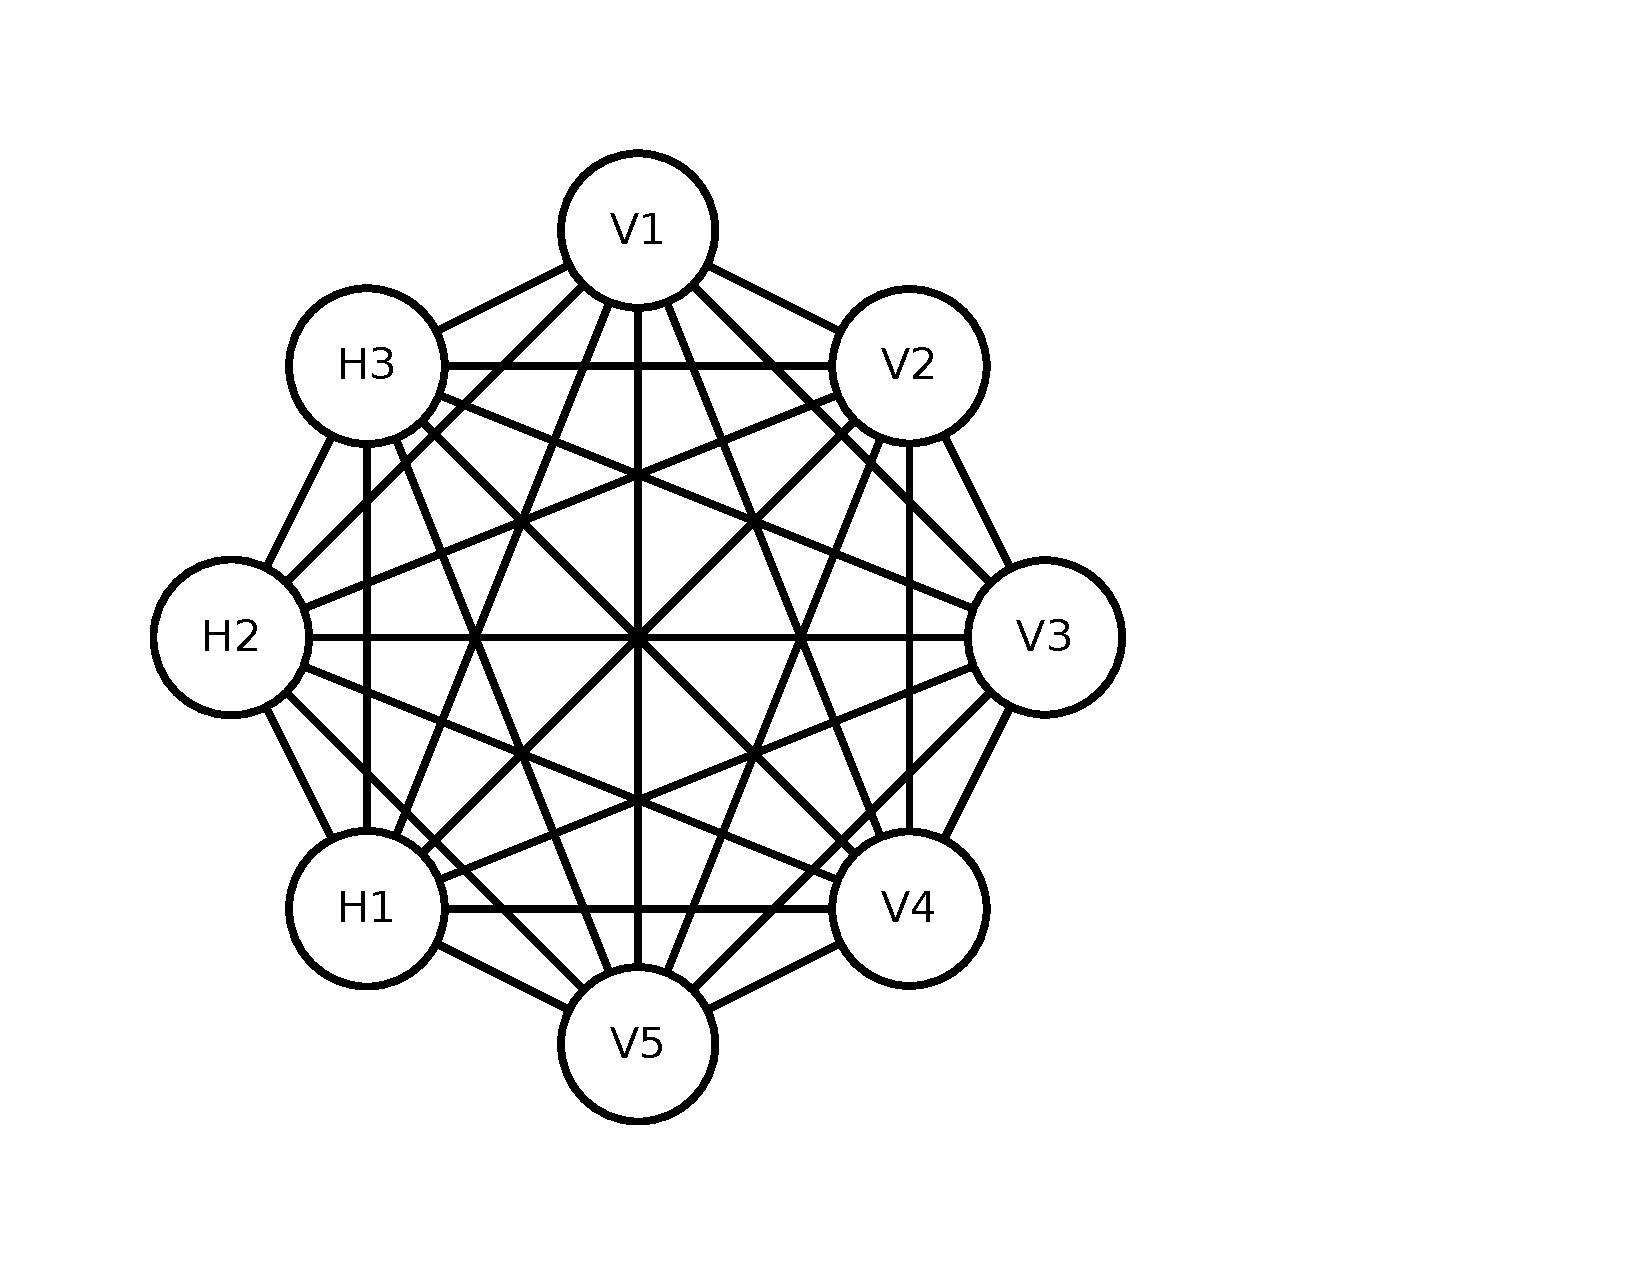
\includegraphics[width=0.6\columnwidth]{images/boltzmann-machine-example}
\par\end{centering}
\caption[A schematic example of a Boltzmann Machine.]{\label{fig:Boltzmann-Machine-schema}A schematic example of a Boltzmann
Machine.  There are visible nodes V1 to V5 and hidden nodes H1 to
H3, each of which have a real-valued bias. Pairs of nodes are connected
with an undirected and real-valued weight. All pairs of nodes can
be connected by a weight different from 0, but self-connections are
not allowed. A Boltzmann Machine stores a joint probability distribution
(see text).}
\end{figure}

\paragraph{Structure}

A Boltzmann Machine\index{Boltzmann Machine} is a stochastic version
of a Hopfield network. It is an undirected graphical model that has
a specific form of the conditional probability distribution defined
at each node \cite{Neal1992}. A schematic example can be seen in
figure \ref{fig:Boltzmann-Machine-schema}. There are visible nodes
\textbf{$\mathbf{V}$} and hidden nodes $\mathbf{H}$, all of which
have a binary state. The visible nodes correspond to variables in
a training sample, while the hidden nodes model dependencies between
those variables, and can be seen as feature detectors. Any two nodes
$i$ and $j$ may be connected using an undirected connection with
weight $w_{ij}$, with the restrictions that there are no self-connections
($w_{ii}=0$) and all connections are symmetric ($w_{ij}=w_{ji}$).
A Boltzmann Machine stores a joint probability distribution. 

The conditional probability distribution for a hidden node $H_{i}\in\mathbf{H}$
depends on the states of all other nodes $\mathbf{S_{j}}$ and is
defined by \cite{HintonSejnowski1986}  as

\begin{equation}
P(H_{i}=1\mid\mathbf{S_{j}}=\mathbf{s_{j}}:j\neq i)=\sigma\left(\sum_{j}s_{j}w_{ij}-b_{i}\right),\label{eq:Boltzmann Machine p(h=00003D1|S)}
\end{equation}
where $\mathbf{S}=\mathbf{V}\cup\mathbf{H}$, $s_{j}$ is the state
of node $S_{j}$, $\sigma(x)=\frac{1}{1+\exp(-x)}$, $w_{ij}\in\mathbb{R}$
is the weight between hidden node $H_{i}$ and (visible or hidden)
node $S_{j}$, and $b_{i}$ is the bias of hidden node $H_{i}$. Similarly,
\[
P(V_{j}=1\mid\mathbf{S_{i}}=\mathbf{s_{i}}:i\neq j)=\sigma\left(\sum_{i}s_{i}w_{ij}-c_{j}\right),
\]
where $V_{j}$ is a visible node, $w_{ij}=w_{ji}$ is the weight between
node $S_{i}$ and visible node $V_{j}$\footnote{this $w_{ij}$ is the same as in equation \ref{eq:Boltzmann Machine p(h=00003D1|S)}},
and $c_{j}$ is the bias of visible node $V_{j}$.

\paragraph{Gibbs Sampling in Boltzmann Machines}

A Boltzmann Machine is an undirected graphical model. Therefore the
approximate Gibbs sampling inference algorithm from \cite{Neal1993}
applies, which works by iteratively drawing the state of an unknown
variable $s_{i}\in\mathbf{S}=\mathbf{H}\cup\mathbf{V}$ from its conditional
probability distribution, given the states of all other variables
$\mathbf{s_{j:j\neq\mathbf{i}}}$. See section \ref{subsec:Inference-in-Markov-Random-Fields}.

\subsubsection{Training Boltzmann Machines}

The goal of training a Boltzmann Machine is to find parameters,
i.e. weights and biases, such that the probability of the training
data becomes maximal. Remember that Boltzmann Machines store a joint
probability distribution. The log-likelihood is

\begin{eqnarray*}
L & = & \log\prod_{\mathbf{v}\in\mathbf{T}}P(\mathbf{V}=\mathbf{v}),
\end{eqnarray*}
 where $\mathbf{T}$ is the set of training data (to be applied to
the visible nodes) and its derivative with respect to a weight $w_{ij}$
is 
\[
\frac{\partial L}{\partial w_{ij}}=\sum_{\mathbf{v}\in\mathbf{T}}\left(\sum_{\mathbf{s}}P(\mathbf{S=s}\mid\mathbf{V=v})s_{i}s_{j}-\sum_{\mathbf{s}}P(\mathbf{S=s})s_{i}s_{j}\right),
\]
 where $\mathbf{S}$ is $\mathbf{V}\cup\mathbf{H}$, and $s_{i}$
is the state of node $S_{i}$ \cite{Neal1992}. The goal is to find
a delta $\Delta w_{ij}$ for each weight $w_{ij}$, which can be added
to the weight, so that the likelihood for the training sample using
the updated weights $w_{ij}+\Delta w_{ij}$ increases. The derivative
of the log-likelihood with respect to a weight $w_{ij}$ multiplied
by a learning rate\index{learning rate} provides such a delta. This
derivative can be approximated by the difference between two parallel
Gibbs Sampling steps: the \emph{positive phase}, where $P(\mathbf{S=s}\mid\mathbf{V=v})s_{i}s_{j}$
is approximated, and the \emph{negative phase}, where $P(\mathbf{S=s})s_{i}s_{j}$
is approximated \cite{Neal1992}.

\paragraph{Positive Phase}

In the positive phase\index{positive phase} of training a Boltzmann
Machine, the visible nodes $\mathbf{V}$ are clamped (i.e. their state
is held fixed) to their states as they are in the training sample
$\mathbf{v}$, and then the states of the remaining (i.e. hidden)
nodes are sampled via Gibbs Sampling. We start in any (for example
random) configuration of the hidden nodes, repeatedly sample each
remaining variable $S$ from its conditional probability distribution
given the states of all other variables (i.e. $P(S_{i}=s_{i}\mid\mathbf{S_{j}}=\mathbf{s_{j}}:j\neq i)$)
until the Gibbs sampler reaches equilibrium, and record the state
$s_{i}$ that each remaining variable $S_{i}$ had assumed in equilibrium.
By repeatedly sampling the $s_{i}$ a few times $t$ when the Markov
chain is in equilibrium, we determine their probability distributions,
where $t$ depends on the desired resolution of the probabilities.
The conditional probability distribution of the remaining variables
$P(\mathbf{S=s}|\mathbf{V=v})$ is determined. Therefore the term
$\sum_{\mathbf{s}}P(\mathbf{S=s}|\mathbf{V=v})s_{i}s_{j}$ can be
determined, which completes the positive phase.

\paragraph{Negative Phase}

In the negative phase\index{negative phase} no nodes are clamped,
and the states of all variables in equilibrium are recorded. Again,
we start in any configuration of the network. Then we repeatedly sample
from the conditional probability distributions $P(S_{i}=s_{i}\mid S_{j}=s_{j}:j\neq i)$
for all variables $S_{i}$ until equilibrium, and record the state
$s_{i}$ each variable $S_{i}$ had in equilibrium. Sampling a few
more steps in equilibrium, we can determine their distributions $P(\mathbf{S=s})$
and therefore the term $\sum_{\mathbf{s}}P(\mathbf{S=s})s_{i}s_{j}$.

\paragraph{Training Iterations}

The derivatives obtained by the positive and negative phases are multiplied
by the learning rate\index{learning rate} $\epsilon$ (a small positive
real constant) and added to the current weights
\[
w_{ij}^{(t+1)}=w_{ij}^{(t)}+\epsilon\frac{\partial L}{\partial w_{ij}}=w_{ij}^{(t)}+\Delta w_{ij}^{(t)}.
\]
Then another training iteration is started. This is repeated until
the derivatives all converge to zero.

\paragraph{Connections to other Graphical Models}

\cite{Neal1993} notes that the Boltzmann Machine is a generalization
of the Ising model of ferromagnetism: ``Generalized to allow {[}parameters{]}
to vary from spin to spin, and to allow interactions between any two
spins, the Ising model becomes the ``Boltzmann machine'' of Ackley,
Hinton, and Sejnowski.''

\subsection{Restricted Boltzmann Machines}

\begin{figure}
\begin{centering}
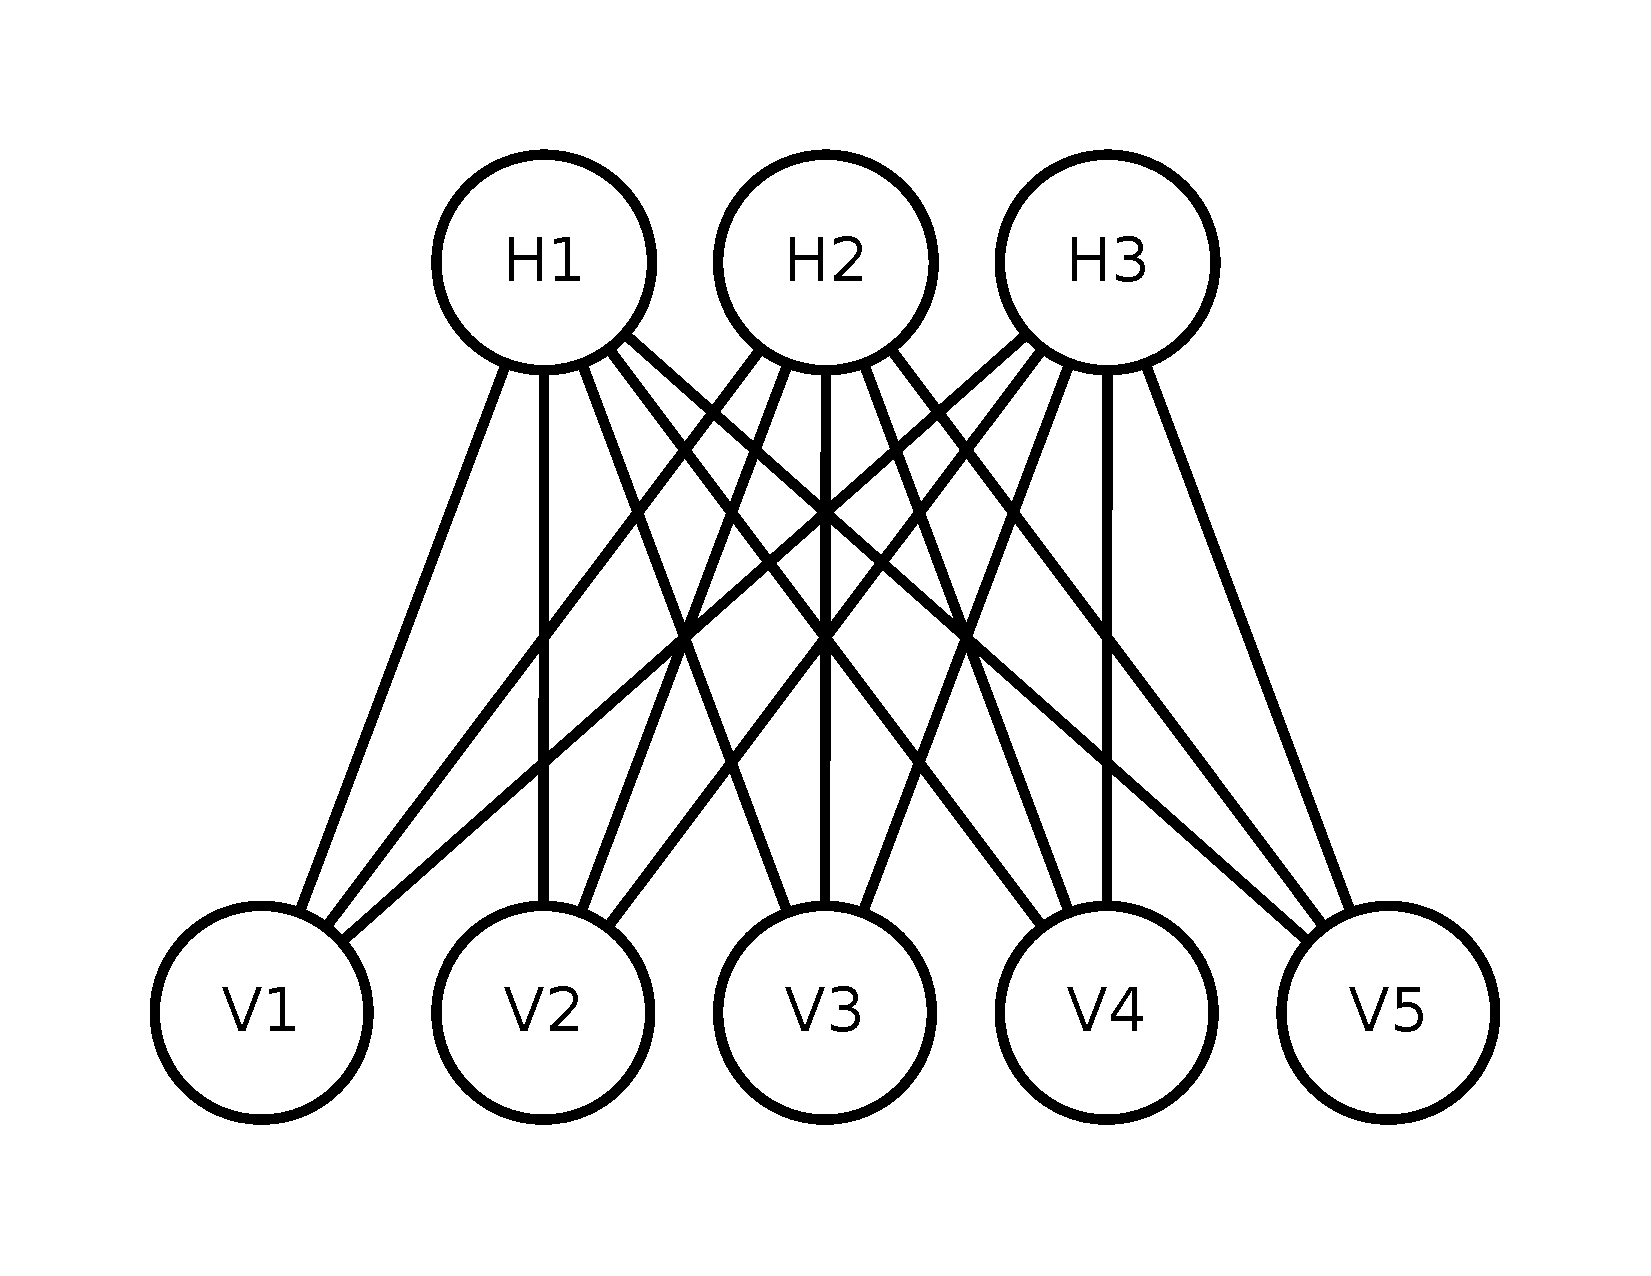
\includegraphics[width=0.55\columnwidth]{images/restricted-boltzmann-machine-example}
\par\end{centering}
\caption[A schematic example of a Restricted Boltzmann Machine.]{\label{fig:Restricted-Boltzmann-Machine-schema}A schematic example
of a Restricted Boltzmann Machine.  There are two layers: the visible
layers with nodes V1 to V5 and the hidden layer with nodes H1 to H3,
each of which have a real-valued bias. Node pairs from different layers
are connected with an undirected and real-valued weight. Connections
between nodes from the same layer and self-connections are not allowed.
A Restricted Boltzmann Machine stores a joint probability distribution
(see text).}
\end{figure}

\paragraph{Structure}

A Restricted Boltzmann Machine\index{Restricted Boltzmann Machine}(RBM\index{RBM})
is a restricted variant of a Boltzmann Machine. Hence, it also is
a way to store a joint probability distribution. An schematic example
of a Restricted Boltzmann Machine can be seen in figure \ref{fig:Restricted-Boltzmann-Machine-schema}.
It has a bipartite topology: there are visible nodes $\mathbf{V}$
and hidden nodes $\mathbf{H}$, and each node in the visible layer
is connected to all hidden nodes by undirected edges, but in contrast
to general Boltzmann Machines no visible-to-visible node connections
and no hidden-to-hidden node connections are allowed. In a Restricted
Boltzmann Machine, the visible nodes represent the observable features
of a training set, while the hidden nodes are feature detectors which
are computed from the states of all visible nodes.

As originally proposed by \cite{Smolensky1986}, a Restricted Boltzmann
Machine has binary visible and hidden nodes. There are extensions
to real-valued nodes, however. See for example \cite{FischerIgel2012}.

The conditional probabilities at the nodes are defined analogous to
Boltzmann Machines (see equation \ref{eq:Boltzmann Machine p(h=00003D1|S)}):

\[
P(H_{i}=1\mid\mathbf{V}=\mathbf{v})=\sigma\left(\sum_{j}v_{j}w_{ij}-b_{i}\right)
\]
\[
P(V_{j}=1\mid\mathbf{H}=\mathbf{h})=\sigma\left(\sum_{i}h_{i}w_{ij}-c_{j}\right),
\]
 where $H_{i}$ is the binary state of hidden node $i$, $\sigma(\cdot)$
is the sigmoid function, $j$ is an index over all visible nodes,
$v_{j}$ is the state of visible node $j$, $w_{ij}$ is the weight
of the connection between hidden node $i$ and visible node $j$,
$b_{i}$ is the bias of hidden node $i$, and $V_{j}$ is the state
of visible node $j$, $i$ is an index over all hidden nodes, $h_{i}$
is the state of hidden node $i$, and $c_{j}$ is the bias of visible
node $j$.


\subsubsection{Contrastive Divergence Learning \label{subsec:Training-Restricted-Boltzmann-Machines-using-Contrastive-Divergence}}

A Restricted Boltzmann Machine is a restricted form of the more general
Boltzmann Machine. Therefore, it can be trained using the training
procedure for Boltzmann Machines. However, there is also a more direct
learning procedure called \emph{contrastive divergence}\index{contrastive divergence},
where the positive phase is simpler, because the hidden and visible
nodes are conditionally independent, given the nodes of other type.
Contrastive divergence is obtained by approximating the derivative
of the log-likelihood with respect to a weight $w_{ij}$.

Like for Boltzmann Machines, the goal of training is to find parameters
such that the probability of the training data becomes maximal. The
log-likelihood is 
\begin{eqnarray*}
L & = & \log\prod_{\mathbf{v}\in\mathbf{T}}P(\mathbf{V}=\mathbf{v}),
\end{eqnarray*}
 where $\mathbf{T}$ is the set of training data (to be applied to
the visible nodes) and its derivative with respect to a weight $w_{ij}$
is 
\begin{equation}
\frac{\partial L}{\partial w_{ij}}=\sum_{\mathbf{v}\in\mathbf{T}}\left(P(H_{i}=1\mid\mathbf{V=v})v_{j}-\sum_{\mathbf{v}}P(\mathbf{V=v})P(H_{i}=1\mid\mathbf{v})v_{j}\right)\label{eq:RBM-contrastive-divergence}
\end{equation}
 (see e.g. \cite{FischerIgel2012}). The difference in equation \ref{eq:RBM-contrastive-divergence}
is called the difference between the \index{positive phase}\emph{positive
}and \index{negative phase}\emph{negative phase}.

\paragraph{Positive Phase}

The positive phase, i.e. $P(H_{i}=1\mid\mathbf{V=v})v_{j}$ can be
computed directly by setting the visible nodes to the training sample,
and then computing $P(H_{i}=1\mid\mathbf{V=v})=\sigma\left(\sum_{j}v_{j}w_{ij}-b_{i}\right)$.
Multiplying by $v_{j}$ completes the positive phase of computing
the delta for $w_{ij}$.

\paragraph{Negative Phase}

The negative phase $\sum_{\mathbf{v}}P(\mathbf{V=v})P(H_{i}=1\mid\mathbf{v})$
is not as straightforward to compute. It may be approximated by running
a Gibbs chain until convergence. We first initialize the network with
any state, then alternatingly compute $P(\mathbf{H}\mid\mathbf{V})$
and $P(\mathbf{V}\mid\mathbf{H})$ until the stationary distribution
is reached. The number of iterations is $k$ and the gradient computed
by contrastive divergence\index{contrastive divergence} (i.e. the
difference of positive phase and negative phase) is called $CD_{k}$.
Often $k=1$ is used at the beginning of training and later $k$ is
incremented. $\mathbf{v}$ and $\mathbf{h}$ are sampled from the
stationary distribution and allow computing $\sum_{\mathbf{v}}P(\mathbf{V=v})P(H_{i}=1\mid\mathbf{v})v_{j}$.


\subsubsection{Parameters of Training a Restricted Boltzmann Machine}

In addition to the parameters for training a Multilayer Perceptron,
i.e. the amount of momentum, the choice of the activation function,
and how to randomly initialize weights and biases (see section \ref{subsec:Parameters-of-Training-a-Multilayer-Perceptron}),
there are the following:

\paragraph{Interpreting the Output of a Node as a Continuous Value}

The output of a node in a Restricted Boltzmann Machine is binary (i.e.
either 0 or 1). However the sigmoid activation function outputs continuous
values between 0 and 1. This output of the sigmoid activation function
is interpreted as the probability that the node outputs value 1, and
0 otherwise. Using this output value directly, without sampling from
a binomial distribution, allows the output to be from the interval
$\{0,1\}$.

\paragraph{Linear nodes with independent Gaussian noise}

\cite{HintonSalakhutdinov2006} proposed a way to extend Restricted
Boltzmann Machines with only binary values to nodes with real values.
However, this extension was largely replaced by rectified linear nodes
because they performed better.

\paragraph{Rectified linear activation function\label{par:Rectified-linear-activation-function}}

\cite{NairHinton2010} then modified the idea in \cite{HintonSalakhutdinov2006}
to rectified linear nodes, in which the sampled output of a node is
given by $\max(0,x+N(0,\sigma(x))$ where $x$ is the sum of the inputs
of the node, $\sigma(x)$ is the sigmoid function, and $N(0,\sigma(x))$
is normally distributed noise with mean $0$ and variance $\sigma(x)$.
This allows using any positive real value for the random variables
of a RBM.


\subsection{Deep Belief Networks\label{subsec:Deep-Belief-Network}}

\paragraph{Structure}

\index{Belief network}Belief Network is another name for directed
graphical model. \emph{Deep Belief Networks}\index{Deep Belief Network}
(DBNs\index{DBN}) are Belief Networks in which the nodes are organized
in layers, and where the value of a node in a layer only depends on
the values of nodes in the layer above. There are no loops in Deep
Belief Networks. The word ``deep'' refers to the number of (more
than a few) hidden layers of a Deep Belief Network. Deep Belief Networks
can be seen as the stochastic counterpart of deterministic feed-forward
networks.

Deep Belief Networks are directed graphical models, therefore the
computation of the values of children nodes does not affect the value
of parent nodes. In contrast to undirected graphical models, this
allows generating (drawing a sample) from the model in a single pass.
Thus, a Deep Belief Network can be used in an unsupervised algorithm
to generate samples distributed like a training data set.

\paragraph{Sigmoid Belief Networks}

Sigmoid Belief Networks were defined by \cite{Neal1992} as a directed
graphical model with a sigmoid conditional probability function. A
Sigmoid Belief Network is a Belief Network in which the conditional
probability associated with node $N_{i}$ depends only on previous
nodes $\mathbf{N_{j}}$ (where parents must come before children).
The conditional probabilities can be expressed as a sigmoid function
\begin{eqnarray*}
P(N_{i} & = & 1_{i}\mid\mathbf{N_{j}=n_{j}}:j<i)=\sigma(\sum_{j<i}n_{j}w_{ij}-b_{i}),
\end{eqnarray*}
 where $n_{j}$ is the binary state of node $N_{j}$, $w_{ij}$
is the directed weight from node $N_{j}$ to node $N_{i}$, and $b_{i}$
is the bias of node $N_{i}$. Thus the conditional probabilities of
a Sigmoid Belief Network are parameterized with the weights and biases.

\paragraph{Arbitrary Modelling Capability}

Both Boltzmann machines and Sigmoid Belief Networks can represent
arbitrary probability distributions over a set of an arbitrary number
of visible nodes, provided that a sufficient number of hidden nodes
is available \cite{Neal1992}. However, as \cite{Hastad1987} showed,
a network with one hidden layer less needs up to an exponential factor
more hidden nodes. Thus, a Deep Belief Network with the same total
number of hidden nodes needs less computation steps to draw from a
probability distribution.

\subsubsection{Training Samples Viewed as Generated by a Deep Belief Network}

\begin{figure}[t]
\begin{centering}
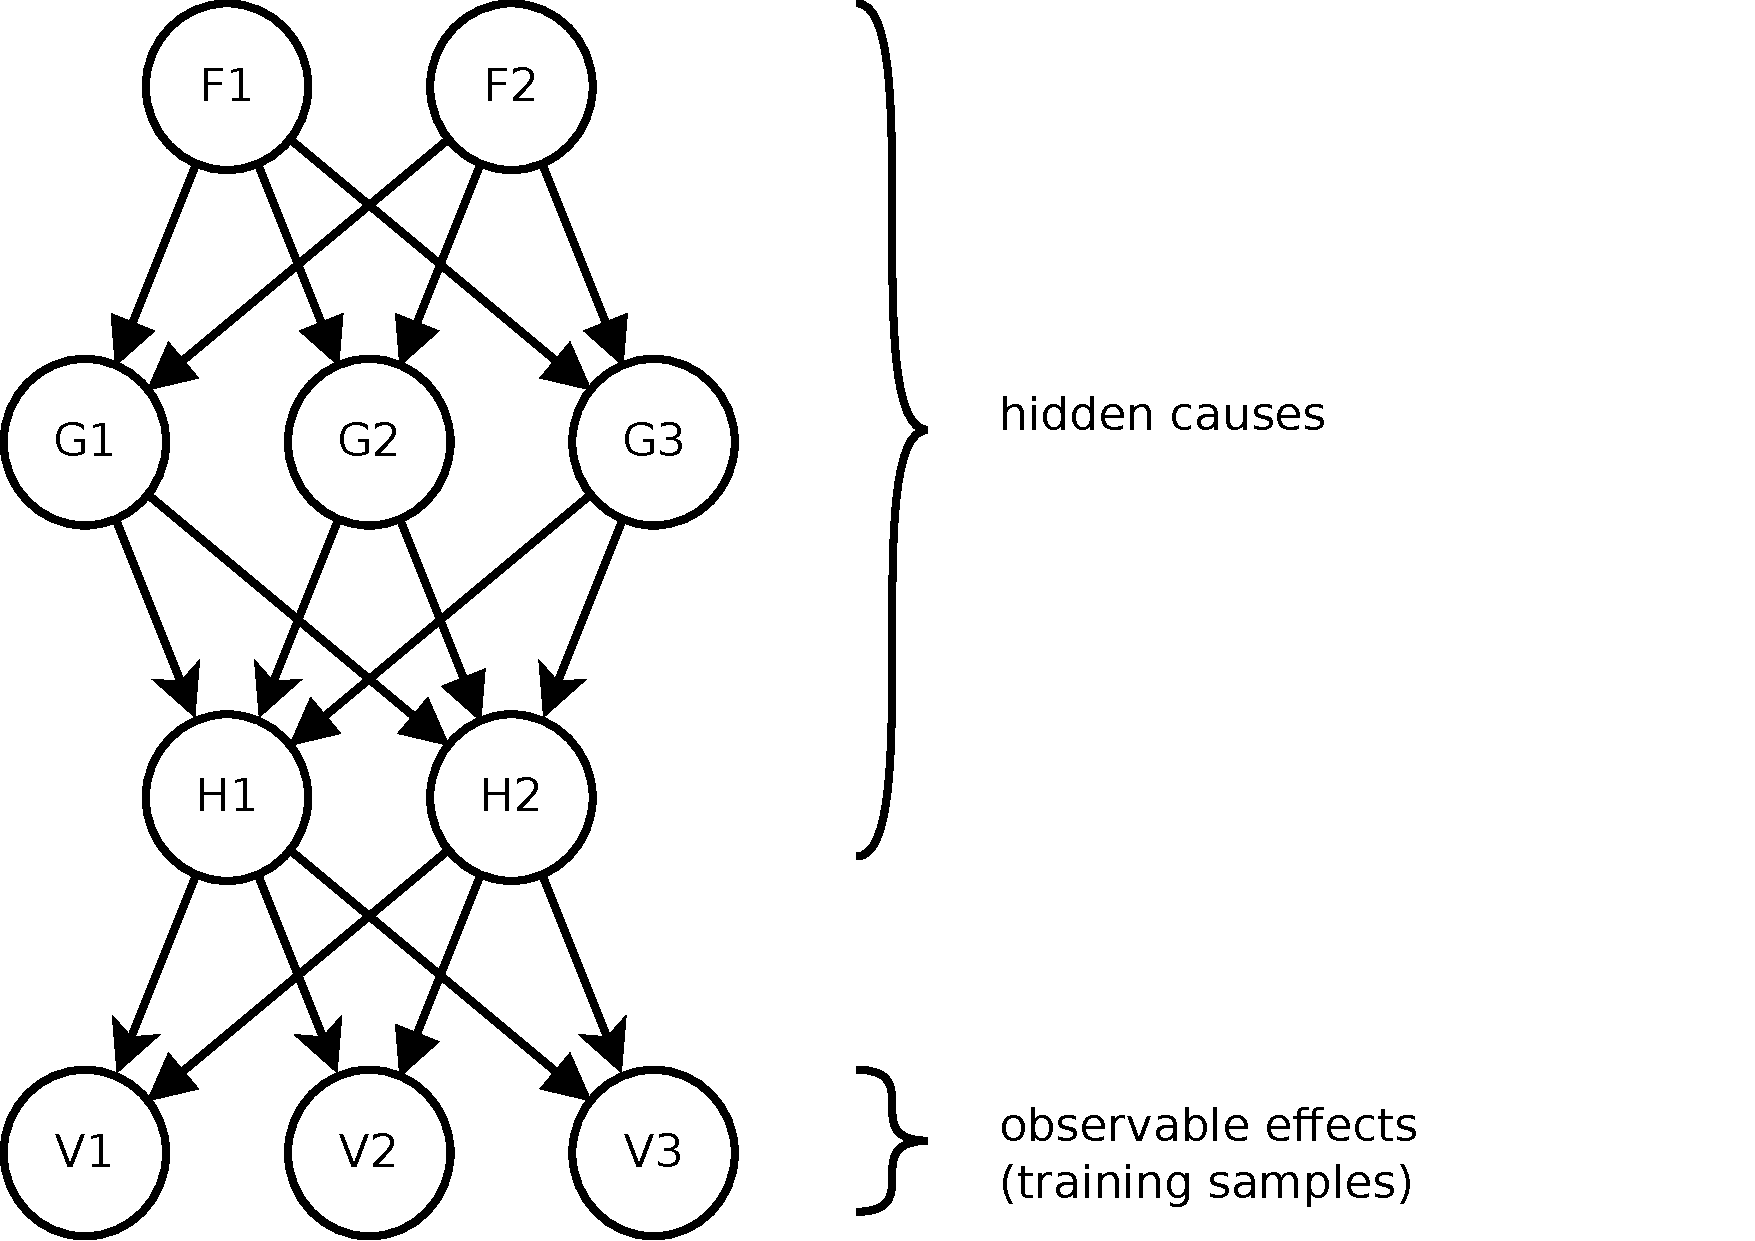
\includegraphics[width=0.50\paperwidth]{images/deep-belief-network}
\par\end{centering}
\caption[Training a Deep Belief Network]{\label{fig:training-a-DBN}The training samples are generated by
a Deep Belief Network, a directed graphical model. In the depicted
example, the top layer $\mathbf{F}$ consists of the random variables
that represent the causes, leading to an observable training sample
in the bottom layer $\mathbf{V}$. The distribution of a random variable
in the layers below the first ($\mathbf{G}$, $\mathbf{H}$, and $\mathbf{V}$)
is determined by the states of the random variables in the layer above.
Only the states of the random variables in the bottom visible layer
$\mathbf{V}$ are observable. Training a Deep Belief Network means
finding weights for the connections between the layers and biases
for each variable, so that the whole model could have generated the
training data.}
\end{figure}
Training a Deep Belief Network is unsupervised, and we have unlabeled
training data consisting of a set of vectors $\mathbf{v_{p}}$, each
with the same dimension. (Hence the training data can be represented
by a matrix.) We view these training samples as being the result of
the probabilistic evaluation of a Deep Belief Network. This is depicted
in figure \ref{fig:training-a-DBN}. Unsupervised training of a Deep
Belief Network means finding weights between hidden and visible nodes
such that the likelihood given the training samples becomes maximal.

\paragraph{Gradient Ascent of the Whole Model is Infeasible}

We could try doing gradient ascent of the whole model. \cite{Neal1992}
showed that this would mean computing the derivative of the likelihood
$L$ with respect to a weight $w_{kj}$ of the connection from node
$j$ to node $k$ 
\[
\frac{\partial L}{\partial w_{kj}}=\sum_{\mathbf{h}}P(\mathbf{H}=\mathbf{h}\mid\mathbf{V}=\mathbf{v})h_{j}\sigma\left(-h_{k}\sum_{i}h_{i}w_{ji}\right),
\]
 where $\mathbf{H}=(H_{i})_{i=1,..n}$ are the nodes from layers above
the visible layer, $\mathbf{h}=(h_{i})_{i=1,..n}$ are their states,
$\mathbf{V}$ and $\mathbf{v}$ are the visible nodes and their states,
$h_{j}$ is the state of node $j$, and $h_{i}$ is the state of node
$i$, which is in the layer above node $j$. In the derivative we
would have to evaluate the conditional probability $P(\mathbf{H}=\mathbf{h}\mid\mathbf{V}=\mathbf{v})$,
which is an inference problem. However, exact inference of the hidden
nodes given the visible nodes is intractable. Therefore we would have
to resort to approximate Gibbs Sampling. This would work by alternatingly
updating each random variable using the conditional probability of
the variable given all other variables (see page \pageref{par:Gibbs-Sampling-in-Markov-Random-Fields}).
However, in Gibbs Sampling, all hidden variables (of all layers simultaneously)
are inferred together (at the same time), and this scales poorly as
models become larger. Therefore another learning algorithm is needed.

\subsubsection{A Fast Learning Algorithm for Deep Belief Networks\label{subsec:A-Fast-Learning-Algorithm-for-Deep-Belief-Networks}}

\cite{HintonTeh2006} showed that there is a fast greedy learning
algorithm for Deep Belief Networks, even with many hidden layers and
millions of parameters. It does not train the weights between all
layers at once, but starts with the weights between the lowest two
layers, and iteratively adds layers and their weights.

There are computational problems with inferring the hidden variables
from visible ones: Inference requires marginalizing out all variables
of a layer except one due to explaining away, and it requires integrating
over all variables above that layer (see section \ref{par:Exact-Inference-in-Deep-Belief-Networks-is-Complicated}).
In addition, updating a weight requires knowing all weights above
in the network. The problems would go away if the posterior of the
hidden given the visible nodes were independent between individual
hidden nodes, because this would eliminate explaining away.

Hence, \cite{HintonTeh2006} came up with a trick: The posterior is
equal to the product of prior times likelihood. If the prior were
so that it would cancel the correlations of the likelihood, then the
product would factor according to the hidden nodes $\mathbf{H}$ 
\[
P(\mathbf{H}\mid\mathbf{V})=\prod_{i}P(H_{i}=h_{i}\mid\mathbf{V}),
\]
 where $\mathbf{V}$ are the visible nodes. They showed that such
\emph{complementary }priors\index{complementary prior} exist and
are a functional family of the form
\[
P(\mathbf{H})=\frac{1}{C}\exp\left(\log\Omega(\mathbf{h})+\sum_{i}\alpha_{i}(h_{i})\right),
\]
 where $C$ is a normalization constant, $\Omega$ is a function of
the states of the hidden variables and the $\alpha_{i}$ are functions
depending on the hidden states individually. In the desired factorial
form of the posterior all the $H_{i}$ must be conditionally independent
(given visible variables $\mathbf{V}$). By the Hammersley-Clifford
theorem (see \ref{par:The-Hammersley-Clifford-theorem-of-Undirected-Graphical-Model})
these conditions are fulfilled in an undirected graphical model that
has edges between a hidden and a visible variable and edges between
all visible nodes with a joint probability of the form
\begin{equation}
P(\mathbf{V},\mathbf{H})=\frac{1}{C}\exp\left(\sum_{i}\Phi_{i}(\mathbf{v},h_{i})+\beta(\mathbf{v})+\sum_{i}\alpha_{i}(h_{i})\right).\label{eq:DBN-joint-probability-with-dependencies-between-visible}
\end{equation}
For reasons that will be explained in a moment, we also want to get
rid of the edges (i.e. dependencies) between the visible nodes. The
conditional probabilities are then of the form
\begin{equation}
P(\mathbf{H}\mid\mathbf{V})=\prod_{i}P(h_{i}\mid\mathbf{v}).\label{eq:DBN-y-given-x}
\end{equation}

\begin{equation}
P(\mathbf{V}\mid\mathbf{H})=\prod_{k}P(v_{k}\mid\mathbf{h})\label{eq:DBN-x-given-y}
\end{equation}
Also by the Hammersley-Clifford theorem, the joint probability then
specializes from equation \ref{eq:DBN-joint-probability-with-dependencies-between-visible}
to
\[
P(\mathbf{V},\mathbf{H})=\frac{1}{C}\exp\left(\sum_{i}\Phi_{i}(\mathbf{v},h_{i})+\sum_{k}\gamma_{k}(v_{k})+\sum_{i}\alpha_{i}(h_{i})\right).
\]

The reason we wanted to have both independencies as encoded by equations
\ref{eq:DBN-x-given-y} and \ref{eq:DBN-y-given-x} is that these
are the (in)dependecies described by a Restricted Boltzmann Machine.
Inference in an RBM works by repeatedly and alternatingly evaluating
these two conditional probabilities. The correctly inferred distribution
is obtained once the Markov chain reaches equilibrium in iterating.
However, we can also view this iterative inference as taking place
in an infinitely deep directed graphical model that has alternating
visible and hidden layers and has shared (``tied'') weights\index{tied weights}
at all layers. The weights matrix between the layers in the directed
graphical model are $W$ from hidden to visible and $W^{T}$ from
visible to hidden layers.  It is this idea of unrolling the RBM in
time that gives rise to the following training procedure for the weights
of a Deep Belief Network.

\paragraph{The Greedy Training Procedure}

The idea is to train a stack of Restricted Boltzmann Machines, where
in each individual RBM, the hidden nodes infer features derived from
the visible nodes, and serve as input to be used in the visible layer
of the next RBM in the stack. Training starts with a single RBM, whose
visible variables are set to a training sample. After training it
to represent the joint probability distribution of the whole training
data set, we obtain, for each training sample, the states of the hidden
nodes. These hidden features comprise a new training data set, to
be used in the next RBM. Iteratively deriving new features and using
these to train the next RBM, we therefore obtain parameters for each
RBM in the stack.

We will now more formally describe the training procedure. At the
first layer, start with a single RBM containing visible nodes $\mathbf{V}$
and hidden nodes $\mathbf{H_{0}}$ and train it using contrastive
divergence to learn the weights $W_{0}$. Use these weights in the
first layer of the Deep Belief Network. Split each of the undirected
connections between $\mathbf{V}$ and $\mathbf{H_{0}}$ into a connection
going upwards and one going downwards. The upward weights $W_{0}^{T}$
serve the purpose of inferring the $\mathbf{H_{0}}$ representation
of the training data, and the downward weights $W_{0}$ are generative
and part of the model.

Then infer a training data set for another RBM on hidden layers $\mathbf{H_{0}}$
and $\mathbf{H_{1}}$. This RBM needs training data in $\mathbf{H_{0}}$,
but our training samples are for layer $\mathbf{V}$. The \emph{re-representation}\index{re-representation of training samples}
works by placing a training sample into the $\mathbf{V}$ nodes, and
then the upward connections are used to get a new representation of
the data at $\mathbf{H_{0}}$. This is done for all training samples.

We now place an RBM between hidden layers $\mathbf{H_{0}}$ and $\mathbf{H_{1}}$.
Up to now the model is equivalent to running the RBM for one more
iteration, which is implemented by the extra directed layer below
the RBM. This is because the weights between the two sets of layers
are constrained to be equal. Now ``untie'' the upward weights\index{untied weights}
$W_{0}^{T}$ between $\mathbf{V}$ and $\mathbf{H_{0}}$ from the
weights $W_{i}$ (where $i>0$), which are constrained to be the same.
Train the RBM between $\mathbf{H_{0}}$ and $\mathbf{H_{1}}$ on the
converted training samples, obtaining new weights $W_{1}$. As we
untied the weights $W_{0}^{T}$ from $W_{1}$, the inferring weights
$W_{0}^{T}$ between $\mathbf{V}\rightarrow\mathbf{H_{0}}$ became
incorrect in theory. In practice, however, this does not matter that
much. As \cite{HintonTeh2006} note, the gain by training the RBM
on top of re-represented data outweighs the incorrectness of inference.
They argue that the greedy algorithm is guaranteed to improve the
generative model, because $P(\mathbf{V})$ has a lower bound that
increases (or stays the same for a fully trained model) when training
an additional layer. This guarantee is given only for maximum likelihood
Restricted Boltzmann Machine learning. In practice we use contrastive
divergence ($CD$) for speed. However, the guarantee still holds if
we use $CD_{k}$ with a large enough number of iterations $k$.

The greedy algorithm now proceeds iteratively, i.e. the steps of inferring
a training data set for a deeper layer and training an RBM on this
data continue until the model is sufficiently deep. Above, we constrained
the model to have an equal number of nodes in each layer. The greedy
training procedure also works for layers of different sizes. Thus
training using gradient descent and approximate Gibbs Sampling, which
is feasible only for a few layers and variables, can be replaced by
the tractable greedy algorithm.

\subsubsection{Deep Belief Networks Interpreted as Feed-forward Neural Networks}

\paragraph{Pre-training}

A trained DBN can be reinterpreted as a feed-forward neural network.
In particular, the weights and biases of an unsupervisedly trained
DBN can be transferred to a multi-layer feed-forward neural network
with the same architecture as the DBN, thereby making the stochastic
DBN a deterministic neural network.  The process of training a DBN
using stacks of RBMs, and transferring the weights and biases is called
\emph{pre-training}\index{pre-training}.

\paragraph{Fine-tuning}

Furthermore, another neural network can be put on top of the pre-trained
converted DBN, where the final (output) layer has neurons corresponding
to variables to be predicted. Usually the network consists of only
one layer, due to difficulties in training freshly initialized multi-layer
neural networks. The resulting network can then be \emph{fine-tuned}\index{fine-tuning},
using standard back-propagation, into a configuration that can predict
from input variables (input at the bottom of the network) the output
variables (read off at the top of the network).

\paragraph{Re-representation of the Data}

In such a composite structure, the (unsupervisedly trained) DBN weights
take on the responsibility of re-representing the data so that it
is in an abstracted form that is easier to learn on. Correlated variables,
for example, are represented by a single variable indicating whether
a feature is present in the sample or not. The (supervisedly trained)
weights on top of the network have the responsibility to label the
sample, i.e. indicate whether the abstracted representation of the
sample is of a certain form or not.




\cleardoublepage{}

\part{Results}


\section{General Remarks}

\subsection{Treatment Sensitivity Prediction for Personalized Medicine}

The goal of personalized medicine is to provide custom-tailored medicine
to every patient. An essential part of this is to select an appropriate
treatment for a specific patient out of the available treatments.
The treatment should have a high probability of succeeding. One way
of approaching this is through machine learning on the expression
data from a patient's tissue to predict treatment outcome. Such a
prediction requires similar expression data from multiple patients
that already underwent the treatment and where the therapy outcome
is known.

In order to evaluate the usefulness of deep learning in the context
of personalized medicine, we analyzed a data set that had something
to do with drug sensitivity and resistance. GSE25055 and GSE25065
are microarray expression data sets produced for the same paper, namely
\cite{HatzisSymmans2011}. Table \ref{tab:GSE25055-GSE25065-sample-number}
shows the number of samples of each label in both data sets. The authors
used GSE25055 to generate a classifier for the prognosis of breast
cancer patients that received reductive surgery preceded by taxane-anthracycline
chemotherapy. All patients had ERBB2 (also called HER2 or HER2/neu)-negative
breast cancer. From each patient, tissue was extracted in reductive
surgery and measured for genome-wide gene expression on Affymetrix
HG-U133A microarrays. 

After an observation period of a couple of years, the mean of which
was 3 years, the patients were labeled as either showing \emph{pCR}\index{pCR}
or \emph{RD}\index{RD} to chemotherapy. \emph{pCR }is an abbreviation
of \emph{pathologic complete response}\index{pathologic complete response}
and means that there was no sign of a remaining breast cancer. In
the following it will be labeled as ``class 1'' or ``label 1''.
\emph{RD} abbreviates \emph{residual disease}\index{residual disease}
and means there was still cancerous tissue. It will be termed ``class
0'' or ``label 0''.

\cite{HatzisSymmans2011} then tested their classifier on an independently
measured data set, GSE25065. The input to the prediction was the expression
data and the desired output a label of either \emph{RD }or \emph{pCR}.

\begin{table}
\begin{centering}
\begin{tabular}{|c|c|c|c|c|}
\hline 
 & label 0, RD & label 1, pCR & label NA & $\sum$\tabularnewline
\hline 
\hline 
GSE25055 & 249 & 57 & 4 & 310\tabularnewline
\hline 
GSE25065 & 140 & 42 & 16 & 198\tabularnewline
\hline 
\end{tabular}
\par\end{centering}
\caption[Number of samples in GEO datasets GSE25055 and GSE25065.]{\label{tab:GSE25055-GSE25065-sample-number}Number of samples in
GEO datasets GSE25055 and GSE25065. ``label 0, RD'' means ``residual
disease''; ``label 1, pCR'' means ``pathologic complete response''.
``label NA'' means that microarray data for the patient is available,
but not his/her disease status.}
\end{table}

\subsection{Goal of this Work}

The context of this work is the use of classifiers on high-dimensional
data as supporting tools for treatment decisions. Three types of neural
networks that lend themselves to semi-supervised training were used:
autoencoders, Restricted Boltzmann Machines and Deep Belief Networks.
Parallel to these, the performance of a semi-supervised version of
Support Vector Machines, namely the Transductive SVM was evaluated.

The specific goals were:
\begin{enumerate}
\item to find out whether incorporating unlabeled expression data in the
training of deep artificial neural networks enhances a classifier's
performance.
\item to assess performance of the classifier on an independently measured
data set.
\item to evaluate whether artificial neural networks can compete with established
classification algorithms like SVMs.
\end{enumerate}

\subsection{How Unlabeled Data Was Used in Training}

In the following, we will discuss how we used unlabeled data in semi-supervised
training.

\subsubsection{How Unlabeled Data was Used in Pre-Training Autoencoders and Fine-tuning
Using Back-propagation}

Autoencoders\index{autoencoder} are composed of an encoder\index{encoder}
and a decoder\index{decoder}. The encoder tries to compress the input
data and the decoder tries to reconstruct the input from its compressed
form. Training autoencoders is unsupervised. As a general rule only
the samples designated as ``unlabeled'' were used in training the
unsupervised part of an algorithm.

The decoder network of the trained autoencoder was then discarded,
so that only the encoder remained. Classification was done on the
compressed representation of the input. The classifier network was
built on top of the encoder (see figure \ref{fig:supervised-network-on-top-of-unsupervised}),
and the compressed output layer of the encoder was used as the input
layer of the classifier.

\begin{figure}
\begin{centering}
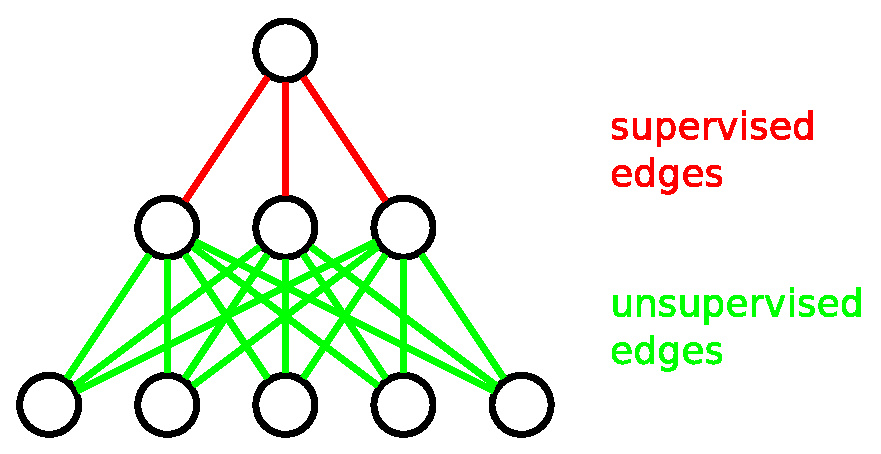
\includegraphics[width=0.35\paperwidth]{images/progress_report_201411-unsupervised-to-supervised}
\par\end{centering}
\caption[How a supervised network is trained on top of a pre-trained unsupervised
network.]{\label{fig:supervised-network-on-top-of-unsupervised}Example scheme
showing how the supervised network is trained on top of a pre-trained
unsupervised network. The network receives input from the bottom,
and the resulting label is read off at the top. The unsupervised network
can be more than 2 layers deep. It is trained first during pre-training.
Then the supervised network is appended onto the top and trained together
with the unsupervised network.}
\end{figure}

The weights of the classifier were initialized randomly, and standard
back-propagation was used to train the whole network to classify samples.
Hence, the encoder can be modified by back-propagation training, but
pre-training with the autoencoder initializes it to a configuration
that ``knows'' about the unlabeled samples. The learning rate of
the second training run (\emph{fine-tuning}\index{fine-tuning}) should
be small enough not to diverge from the unlabeled training configuration
in too large steps (per iteration).

Algorithm \ref{alg:pretrain-autoencoder-finetune-backprop} shows
the pseduo-code for pre-training using a DBN and fine-tuning using
backpropagation.

\begin{algorithm}
\begin{enumerate}
\item initialize the autoencoder $A$
\item \label{enu:Autoencoder-for-all-unlabeled-training-data}for all unlabeled
training samples $U$ in the unlabeled training data set:

\begin{enumerate}
\item set the input of $A$ to $U$
\item train $A$ with the goal of reconstructing $U$
\end{enumerate}
\item repeat step \ref{enu:Autoencoder-for-all-unlabeled-training-data}
until the reconstruction error is small enough
\item replace the decoder part of $A$ with a randomly initialized classifier
to form the feed-forward network $C$
\item \label{enu:Autoencoder-for-all-training-pairs}for all labeled training
data, consisting of input samples $X$ and corresponding desired output
sample $Y$ :

\begin{enumerate}
\item set the input of $C$ to $X$
\item train $C$ using back-propagation to output $Y$
\end{enumerate}
\item repeat step \ref{enu:Autoencoder-for-all-training-pairs} until the
classification error is small enough (subject to early stopping or
model selection)
\end{enumerate}
\caption{\label{alg:pretrain-autoencoder-finetune-backprop}Pre-training on
unlabeled data using an autoencoder and backpropagation fine-tuning
with labeled data.}
\end{algorithm}

\subsubsection{How Unlabeled Data was Used When Pre-training a Restricted Boltzmann
Machine and Fine-tuning Using Back-propagation}

When using the unsupervised Restricted Boltzmann Machine to find the
approximate weights of a neural network, the unlabeled data were used
to train the Restricted Boltzmann Machine. The resulting neural network
was then extended with the network layer for supervised classification,
and the complete network was trained using (supervised) back-propagation
on the labeled data. 

Algorithm \ref{alg:pretrain-RBM-finetune-backprop} shows the pseduo-code
for pre-training using a DBN and fine-tuning using backpropagation.

\begin{algorithm}
\begin{enumerate}
\item initialize the Restricted Boltzmann Machine $R$
\item \label{enu:RBM-for-all-unlabeled-training-data}for all unlabeled
training samples $U$ in the unlabeled training data set:

\begin{enumerate}
\item train $R$ with the goal of learning the probability distribution
of $U$
\end{enumerate}
\item repeat step \ref{enu:RBM-for-all-unlabeled-training-data} until the
reconstruction error is small enough
\item put a classifier on top of $R$ to form the feed-forward network $C$
\item \label{enu:RBM-for-all-training-pairs}for all labeled training data,
consisting of input samples $X$ and corresponding desired output
sample $Y$ :

\begin{enumerate}
\item set the input of $C$ to $X$
\item train $C$ using back-propagation to output $Y$
\end{enumerate}
\item repeat step \ref{enu:RBM-for-all-training-pairs} until the classification
error is small enough (subject to early stopping or model selection)
\end{enumerate}
\caption{\label{alg:pretrain-RBM-finetune-backprop}Pre-training on unlabeled
data using a Restricted Boltzmann Machine and backpropagation fine-tuning
with labeled data.}
\end{algorithm}

\subsubsection{How Unlabeled Data was Used in Training Deep Belief Networks}

Deep Belief Networks are an unsupervised algorithm and thus were trained
using unlabeled data. As with Restricted Boltzmann Machines, the
resulting network was then extended with the classifier layer, and
the complete network was fine-tuned using back-propagation on the
labeled data.

Initializing the complete network with the weights and biases of a
trained DBN serves the purpose of initializing the complete network
to a low energy configuration that has a higher chance to be trainable
using back-propagation. It does not prevent back-propagation from
settling in a configuration that is far away from the weights and
biases of the trained DBN.

Algorithm \ref{alg:pretrain-DBN-finetune-backprop} shows the pseduo-code
for pre-training using a DBN and fine-tuning using backpropagation.
It is identical to pre-training using a Restricted Boltzmann Machine
and fine-tuning using back-propagation, except that we pre-train the
$n$ layers of the Deep Belief Network using RBMs on re-represented
data.

\begin{algorithm}
\begin{enumerate}
\item initialize the Deep Belief Network $D$ to a Restricted Boltzmann
Machine with visible and hidden layer sizes equal to the first two
layers of the DBN
\item for layer $l=2\ldots n$ in the Deep Belief Network:

\begin{enumerate}
\item \label{enu:DBN-for-all-unlabeled-training-data}for all unlabeled
training samples $U$ in the unlabeled training data set:

\begin{enumerate}
\item set re-represented data $R$ to the representation of $U$ in layer
$l-1$
\item think of layers $l-1$ and $l$ in $D$ as a Restricted Boltzmann
Machine and train it with the goal of learning the probability distribution
of $R$
\end{enumerate}
\item repeat step \ref{enu:DBN-for-all-unlabeled-training-data} until the
reconstruction error is small enough
\end{enumerate}
\item put a classifier on top of $D$ to form the feed-forward network $C$
\item \label{enu:DBN-for-all-training-pairs}for all labeled training data,
consisting of input samples $X$ and corresponding desired output
sample $Y$ :

\begin{enumerate}
\item set the input of $C$ to $X$
\item train $C$ using back-propagation to output $Y$
\end{enumerate}
\item repeat step \ref{enu:DBN-for-all-training-pairs} until the classification
error is small enough (subject to early stopping or model selection)
\end{enumerate}
\caption{\label{alg:pretrain-DBN-finetune-backprop}Pre-training on unlabeled
data using a Deep Belief Network and backpropagation fine-tuning with
labeled data.}
\end{algorithm}

\subsection{Issues in Running \emph{deepnet}}

\emph{deepnet} is a neural network implementation written by Nitish
Srivastava, which uses a matrix library (called cudamat) written by
Vlad Mnih and Alex Krizhevsky \cite{Deepnet2014}. It can run on graphics
cards (supporting CUDA). Since graphics cards have a highly parallel
architecture, training times are faster. However, because graphics
cards have to process large data, their RAM is more expensive than
normal RAM for PCs. The graphics cards used have 4 GB of RAM installed.
\emph{deepnet} loads all data sets onto the graphics card at the beginning
of the computation. In addition, the parameter matrices have to be
held in memory. However, there is another matrix library (called
eigenmat and with the same interface as cudamat), which runs on the
normal floating-point unit of a normal CPU. Most of the data sets
were trained on a computer that has 256GB of RAM and 32 cores, which
was more than enough for the data sets tested. There was a bug in
this library when run on 64-bit CPUs, which we fixed. The deepnet
version used can be downloaded from \href{https://github.com/moa1/deepnet/tree/nnet}{https://github.com/moa1/deepnet/tree/nnet},
revision 963C.

\subsection{Training Iterations and Evaluations}

We trained both the unsupervised as well as the supervised network
for a pre-determined number of iterations. This number was determined
by a trial training run on the data set in question. The trial training
run was continued as long as we considered the reconstruction error
(for unsupervised training) or accuracy changes (for supervised networks)
of the neural network substantial. There were usually between 100,000
and 1,000,000 iterations (\emph{deepnet} setting \emph{stopcondition.steps}
in train.pbtxt), and we evaluated the neural network after every 500
iterations (\emph{deepnet} setting \emph{eval\_after} in train.pbtxt).
Evaluation means computing the training set, validation set, and testing
set reconstruction error (in unsupervised training) or accuracy (in
supervised training). The neural network itself was saved every 10,000
iterations (\emph{deepnet} setting \emph{checkpoint\_after} in train.pbtxt).

\begin{table}
\begin{centering}
\begin{tabular}{|c|c|c|c|}
\hline 
name of training run & type & architecture & run-time\tabularnewline
\hline 
\hline 
breast\_cancer\_03\_ai & AE & 500-1000-500 & 0.25 h\tabularnewline
\hline 
breast\_cancer\_03\_al & AE & 500-1000-500 & 1.00 h\tabularnewline
\hline 
breast\_cancer\_03\_am & AE & 500-1000-500 & 1.00 h\tabularnewline
\hline 
breast\_cancer\_03\_ao & AE & 500-1000-500 & 0.50 h\tabularnewline
\hline 
breast\_cancer\_04\_bg & RBM & 500-500 & 3.25 h\tabularnewline
\hline 
breast\_cancer\_04\_bh & RBM & 500-1000 & 5.50 h\tabularnewline
\hline 
breast\_cancer\_04\_bi & RBM & 500-1000 & 5.50 h\tabularnewline
\hline 
breast\_cancer\_04\_bj & RBM & 500-1000 & 5.50 h\tabularnewline
\hline 
breast\_cancer\_06\_aa/\_n018\_cv1 & FFN & 500-500-1 & 1.00 h\tabularnewline
\hline 
breast\_cancer\_06\_ab/\_n018\_cv1 & FFN & 500-1000-1 & 2.75 h\tabularnewline
\hline 
breast\_cancer\_06\_ac/\_n018\_cv1 & FFN & 500-1000-1 & 2.75 h\tabularnewline
\hline 
breast\_cancer\_06\_ad/\_n018\_cv1 & FFN & 500-1000-1 & 2.75 h\tabularnewline
\hline 
breast\_cancer\_06\_ae/\_n018\_cv1 & FFN & 500-1000-1 & 0.75 h\tabularnewline
\hline 
breast\_cancer\_06\_af/\_n018\_cv1 & FFN & 500-1000-1 & 0.75 h\tabularnewline
\hline 
breast\_cancer\_06\_ag/\_n018\_cv1 & FFN & 500-1000-1 & 1.00 h\tabularnewline
\hline 
breast\_cancer\_06\_ah/\_n018\_cv1 & FFN & 500-1000-1 & 1.00 h\tabularnewline
\hline 
breast\_cancer\_07\_aa/\_n006\_cv1 & FFN & 500-500-1 & 0.75 h\tabularnewline
\hline 
breast\_cancer\_07\_ab/\_n006\_cv1 & FFN & 500-1000-1 & 1.25 h\tabularnewline
\hline 
breast\_cancer\_07\_ac/\_n006\_cv1 & FFN & 500-1000-1 & 3.00 h\tabularnewline
\hline 
breast\_cancer\_07\_ad/\_n006\_cv1 & FFN & 500-1000-1 & 1.00 h\tabularnewline
\hline 
breast\_cancer\_07\_ae/\_n006\_cv1 & FFN & 500-1000-1 & 1.25 h\tabularnewline
\hline 
breast\_cancer\_07\_af/\_n006\_cv1 & FFN & 500-1000-1 & 2.75 h\tabularnewline
\hline 
breast\_cancer\_07\_ag/\_n006\_cv1 & FFN & 500-1000-1 & 3.00 h\tabularnewline
\hline 
breast\_cancer\_07\_ah/\_n006\_cv1 & FFN & 500-1000-1 & 2.50 h\tabularnewline
\hline 
breast\_cancer\_07\_ai/\_n006\_cv1 & FFN & 500-1000-1 & 0.50 h\tabularnewline
\hline 
breast\_cancer\_07\_aj/\_n006\_cv1 & FFN & 500-1000-1 & 0.50 h\tabularnewline
\hline 
\end{tabular}
\par\end{centering}
\caption[Running times of training selected neural networks, table 1.]{\label{tab:selected-running-times-table1}Selected running times
of training neural networks on data sets breast\_cancer\_03 to breast\_cancer\_07.
Column ``type'' describes the network type trained: ``AE'' means
autoencoder, ``RBM'' means Restricted Boltzmann Machine, ``FFN''
means feed forward network trained using backpropagation. Column ``architecture''
describes the sizes of the layers of the respective network. Column
``run-time'' denotes approximate run-times, and ``h'' means hours.}
\end{table}

\begin{table}
\begin{centering}
\begin{tabular}{|c|c|c|c|}
\hline 
name of training run & type & architecture & run-time\tabularnewline
\hline 
\hline 
breast\_cancer\_08\_bb & AE & 500-1000-500 & 7.00 h\tabularnewline
\hline 
breast\_cancer\_08\_bb & FFN & 500-1000-1 & 4.00 h\tabularnewline
\hline 
breast\_cancer\_08\_bx & AE & 500-1000-500 & 23.00 h\tabularnewline
\hline 
breast\_cancer\_08\_bx & FFN & 500-1000-1 & 6.50 h\tabularnewline
\hline 
breast\_cancer\_08\_by & AE & 500-1000-500 & 7.00 h\tabularnewline
\hline 
breast\_cancer\_08\_by & FFN & 500-1000-1 & 6.50 h\tabularnewline
\hline 
breast\_cancer\_08\_cu & AE & 500-1000-500 & 17.50 h\tabularnewline
\hline 
breast\_cancer\_08\_cu & FFN & 500-1000-1 & 6.00 h\tabularnewline
\hline 
breast\_cancer\_08\_ep & AE & 500-1000-500 & 8.00 h\tabularnewline
\hline 
breast\_cancer\_08\_ep & FFN & 500-1000-1 & 5.50 h\tabularnewline
\hline 
breast\_cancer\_08\_fl & AE & 500-1000-500 & 19.00 h\tabularnewline
\hline 
breast\_cancer\_08\_fl & FFN & 500-1000-1 & 6.50 h\tabularnewline
\hline 
breast\_cancer\_08\_fm & AE & 500-1000-500 & 8.00 h\tabularnewline
\hline 
breast\_cancer\_08\_fm & FFN & 500-1000-1 & 5.45 h\tabularnewline
\hline 
breast\_cancer\_08\_gi & AE & 500-1000-500 & 17.50 h\tabularnewline
\hline 
breast\_cancer\_08\_gi & FFN & 500-1000-1 & 6.15h\tabularnewline
\hline 
breast\_cancer\_12\_aa & DBN1 & 500-1000 & 0.50 h\tabularnewline
\hline 
breast\_cancer\_12\_aa & DBN2 & 500-1000-1000 & 1.75 h\tabularnewline
\hline 
breast\_cancer\_12\_aa & DBN3 & 500-1000-1000-2000 & 2.50 h\tabularnewline
\hline 
breast\_cancer\_12\_aa & FFN & 500-1000-1000-2000-1 & 39.00 h\tabularnewline
\hline 
breast\_cancer\_12\_dv & DBN1 & 500-1000 & 2.25 h\tabularnewline
\hline 
breast\_cancer\_12\_dv & DBN2 & 500-1000-1000 & 6.25 h\tabularnewline
\hline 
breast\_cancer\_12\_dv & DBN3 & 500-1000-1000-2000 & 10.25 h\tabularnewline
\hline 
breast\_cancer\_12\_dv & FFN & 500-1000-1000-2000-1 & 12.25 h\tabularnewline
\hline 
breast\_cancer\_15\_aa & DBN1 & 22283-10 & 2.00 h\tabularnewline
\hline 
breast\_cancer\_15\_aa & DBN2 & 22283-10-10 & 0.25 h\tabularnewline
\hline 
breast\_cancer\_15\_aa & DBN3 & 22283-10-10-10 & 0.25 h\tabularnewline
\hline 
breast\_cancer\_15\_aa & FFN & 22283-10-10-10-1 & 4.00 h\tabularnewline
\hline 
breast\_cancer\_15\_dv & DBN1 & 22283-10 & 11.00 h\tabularnewline
\hline 
breast\_cancer\_15\_dv & DBN2 & 22283-10-10 & 1.50 h\tabularnewline
\hline 
breast\_cancer\_15\_dv & DBN3 & 22283-10-10-10 & 1.50 h\tabularnewline
\hline 
breast\_cancer\_15\_dv & FFN & 22283-10-10-10-1 & 3.50 h\tabularnewline
\hline 
\end{tabular}
\par\end{centering}
\caption[Running times of training selected neural networks, table 2.]{\label{tab:selected-running-times-table2}Running times of training
neural networks on data sets breast\_cancer\_08 to breast\_cancer\_15.
Column ``type'' describes the network type trained: ``AE'' means
autoencoder, ``RBM'' means Restricted Boltzmann Machine, ``FFN''
means feed forward network trained using backpropagation. Column ``architecture''
describes the sizes of the layers of the respective network. Column
``run-time'' denotes approximate run-times, and ``h'' means hours.}
\end{table}

Tables \ref{tab:selected-running-times-table1} and \ref{tab:selected-running-times-table2}
show the approximate training times of selected neural network training
runs. For example, training 100,000 (unsupervised) DBN iterations
of the first hidden layer of classification run breast\_cancer\_15\_aa,
which consists of a 22283-10-10-10-1 network, took 2 hours on 1 core
of the aforementioned 32 cores computer. The second and third hidden
layer took about 15 minutes. Computing 1,000,000 (supervised) back-propagation
iterations of the same run took a little less than 4 hours. The running
time mainly depends on the network architecture, the learning rate,
and number of training iterations. Classifying a sample took about
as long as 1 supervised training iteration and thus was almost instant.

As Transductive Support Vector Machine implementation we used SVMlight,
and as Support Vector Machine implementation we used the R package
e1071 \emph{svm} function \cite{Joachims1999,R2008}. SVMlight and
the R package e1071 \emph{svm} function took a few minutes to train
and classify breast\_cancer\_15\_aa.

\subsection{Model Selection\label{subsec:Model-selection}}

Training an artificial neural network is an iterative process. Hence,
there are as many models as there are iterations. The question is
which one to choose for testing the performance. We did not use ``early
stopping'', i.e. aborting training when the error on the validation
data set becomes too large due to overfitting\index{overfitting},
but selected the neural network that was best on the validation data
among all evaluated iterations.

\paragraph{Select the Most Trained Model for Unsupervised Training}

We normally did not use any model selection for the unsupervised training,
since the reconstruction error plots of pre-training using autoencoder
or RBM did not show overfitting on the validation data set. Instead
we selected the neural network from the last iteration that was computed.
For example, in the plot in figure \vref{fig:reconstruction-errors-of-breast_cancer_04_bg-bj},
we selected the network producing the right-most error.

\paragraph{Select the Model With Best Validation Error for Supervised Training}

We used model selection in training the (supervised) classifiers,
because training a neural network for too many iterations using back-propagation
has the tendency to overfit the training data and generalize poorly
on the validation and test data. Therefore we defined three data sets:
a training data set, which was used to iteratively train the neural
network; a validation data set, which was used to select the model
(see below); and a test data set, which was used to evaluate the accuracy
of the neural network picked using the validation data set.

\paragraph{Smoothing the Accuracies for Model Selection}

Usually model selection means picking the neural network from the
iteration with the highest validation data set accuracy. However,
we sometimes had only few (in the tens) labeled samples in the validation
data set. This led to a very coarse resolution in accuracy plots,
and also to noisy validation data set accuracy plots, which often
jittered between two accuracies from one iteration to the next. See
figure \ref{fig:Example-of-supervised-model-selection} for an example.
We therefore smoothed each of the validation set accuracies, and test
set accuracies using the standard R \emph{loess} smoother with a span
of 0.125. Then we selected the iteration where the smoothed validation
set accuracy was highest, and reported the smoothed test set accuracy
at that iteration. (If there were more than one iteration that had
the highest validation set accuracy, we reported the mean and the
median of the smoothed test set accuracies at these iterations, and
plotted all these accuracies in a box plot.)

\begin{figure}
\begin{centering}
\includegraphics[width=0.5\paperwidth]{images/breast_cancer_15-smoothed_accuracy-at}
\par\end{centering}
\caption[Example of supervised model selection using accuracy smoothing.]{\label{fig:Example-of-supervised-model-selection}Example of supervised
model selection using accuracy smoothing. The x-axis is the training
iteration, the y-axis the accuracy. The turquoise, green, and black
circle clouds are the raw accuracies on the training, validation,
and test set, respectively. They are in discrete steps, because there
are only 20 samples. The thin lines overlayed on the point clouds
are the \emph{loess }smoothed curves used for model selection. The
dashed vertical line is the iteration where the accuracy on the validation
data set is maximal, and the model at that iteration was selected.}
\end{figure}

Note that this procedure allows reporting test set accuracies which
seem impossible. For example in a test set with 10 samples, only an
accuracy in \{0, 0.1, 0.2, ..., 1\} would be possible, but smoothing
allows all rational numbers between 0 and 1 to be returned.

\subsection{Software Used and Parameters}

Besides using \emph{deepnet }by Nitish Srivastava as the neural network
implementation, we used the R CRAN package e1071 \cite{R2008} for
the SVM implementation and TSVM. SVMlight and the R package e1071
\emph{svm} function \cite{Joachims1999,R2008} took a few minutes
to train and classify breast\_cancer\_15\_aa.

The default settings for SVM were used, except the kernel, which was
a linear kernel. In particular, the calls to the svm function were
like the following:

\noindent \begin{verbatim}
SVM <- svm(labeled_training_matrix, labeled_training_labels, kernel="linear")

\end{verbatim}

\noindent The default settings for TSVM were used. In particular,
the command lines were equivalent to the following:

\noindent \begin{verbatim}
echo "learning model"
svm_learn training-input.txt model.model
echo "classifying testing data"
svm_classify testing-input.txt model.model predictions.txt

\end{verbatim}

\subsection{\emph{deepnet }Parameters}

The \emph{deepnet }parameters are set in a configuration file which
first describes default parameters, and then layer-wise parameters
taking precedence over the default parameters, if set. The different
types of parameters are described in the following.
\begin{description}
\item [{\emph{base\_epsilon}}] One of the crucial settings when training
artificial neural networks is the learning rate\index{learning rate}.
It is named \emph{$base\textrm{\_}epsilon$} in \emph{deepnet}. It
controls by what factor the gradient of each weight is multiplied
with to influence the parameters of the neural network in the next
iteration. If it is too large, the neural network will alter weights
in too large steps and oscillate, and will not be able to reach an
energy optimum. If it is too small, learning will take too long.\\
The optimal value can vary greatly between different data sets. It
was selected on each data set separately in neural network training
trials using a grid search. For example, table \ref{tab:Effect-of-learning-rate-on-reconstruction-error}
shows the reconstruction error reached for 5 different learning rates
in a training trial on data set breast\_cancer\_02. In this exemplary
case, 0.01 was a good tradeoff between accuracy and training speed.
However, the optimal learning rate must be determined for each data
set anew. 
\begin{table}
\begin{centering}
\begin{tabular}{|c|c|c|c|}
\hline 
 & \multicolumn{1}{c|}{configs} & \multicolumn{2}{c|}{outputs}\tabularnewline
\hline 
 & base\_epsilon & min. T\_E & note\tabularnewline
\hline 
\hline 
breast\_cancer\_02\_e & 0.0001 & 0.74625 & converging T\_E\tabularnewline
\hline 
breast\_cancer\_02\_d & 0.001 & 0.70599 & converging T\_E\tabularnewline
\hline 
breast\_cancer\_02\_a & 0.01 & 0.70362 & converging T\_E\tabularnewline
\hline 
breast\_cancer\_02\_b & 0.1 & NA & network in a chaotic state\tabularnewline
\hline 
breast\_cancer\_02\_c & 1.0 & 3.2056 & oscillating T\_E\tabularnewline
\hline 
\end{tabular}
\par\end{centering}
\caption[Example of the effect of the learning rate base\_epsilon on reconstruction
error.]{\label{tab:Effect-of-learning-rate-on-reconstruction-error}Example
of the effect of the learning rate base\_epsilon on reconstruction
error. ``T\_E'' is the reconstruction error on the training data
set. ``min T\_E'' is the minimal reconstruction error of 5,100,000
iterations. ``NA'' means not applicable. The table shows that the
learning rate base\_epsilon has a large effect on the minimal reconstruction
error.}
\end{table}
\item [{\emph{activation}}] This is the type of activation function used
for the nodes in the described layer. ``LOGISTIC'' is the sigmoid
activation function (defined on page \pageref{The-sigmoid-activation-function}).
``RECTIFIED\_LINEAR'' is the rectified linear activation function
(see page \pageref{par:Rectified-linear-activation-function}).
\item [{\emph{initial\_momentum},~\emph{final\_momentum},~\emph{momentum\_change\_steps}}] These
are the settings for the momentum of the learning rate, see page \pageref{par:Momentum-of-the-learning-rule}.
The momentum is linearly scaled up from \emph{initial\_momentum} at
iteration 0 to \emph{final\_momentum }at iteration \emph{momentum\_change\_steps}.
\item [{\emph{sparsity},~\emph{sparsity\_target},~\emph{sparsity\_cost},~\emph{sparsity\_damping}}] These
are the parameters of the sparsity regularization. \emph{sparsity}
is either true or false and controls whether sparsity regularization
is used or not, and the other three parameters were described on page
\pageref{subsec:Sparsity-Target}.
\item [{\emph{dropout},~\emph{dropout\_prob}}] \emph{dropout }controls
whether the dropout regularization is enabled or not, and \emph{dropout\_prob
}is the dropout probability, described on page \pageref{subsec:Dropout}.
\item [{\emph{apply\_l2\_decay},~\emph{l2\_decay}}] \emph{apply\_l2\_decay}
controls whether l2 decay regularization is used or not, and \emph{l2\_decay}
is its constant weight cost, described on page \pageref{subsec:L1-and-L2-Weight-Decay}.
\item [{\emph{dimensions}}] This parameter sets the number of nodes in
the described layer.
\item [{\emph{loss\_function}}] If set to ``SQUARED\_LOSS'', the sum
of squared differences is optimized, while ``CROSS\_ENTROPY'' optimizes
the cross entropy. Both are described on page \pageref{par:Optimizing-the-Sum-of-Squared-DIfferences}.
\end{description}

\subsection{Overview Over the Following Sections}

In \textbf{section \ref{sec:Unsupervised-Reconstruction-of-Expression-Values}}
we compress the 10,000 most variable genes of GSE25055 into only 50
numbers and observe only little reconstruction error for most genes.

Then the performance benefit of neural networks using an increasing
number of labeled samples is assessed. The benefit of using more labeled
training samples on testing set accuracy is well-established in machine
learning, and is also observed in \textbf{section \ref{sec:breast_cancer_06-and-breast_cancer_07}}.

In \textbf{section \ref{sec:breast_cancer_08}}, we begin to investigate
the question whether adding unlabeled samples to pre-training improves
the testing set accuracy. To diminish the possibility that the input
to the algorithms does not contain the information required for prediction,
we measure prediction accuracy after using four normalization methods:
Robust Multi-Chip Average (RMA) \cite{BolstadSpeed2003}, and MAS5
\cite{Affymetrix2001}, without and with subsequent ComBat batch-effect
correction \cite{JohnsonRabinovic2007}.

In \textbf{section \ref{sec:breast_cancer_12}}, we use Deep Belief
Networks instead of RBM and autoencoder used previously for pre-training,
and systematically compare SVM, TSVM, and supervised and semi-supervised
neural network variants.

Finally, in \textbf{section \ref{sec:breast_cancer_15}}, we drastically
reduce the number of neural network parameters by reducing the number
of hidden nodes compared to the previous networks. At the same time,
we increase the number of input genes from the 500 most variable genes
to all 22,283 genes.

As we will see, only the attempts with artificial neural networks
in section \textbf{\ref{sec:breast_cancer_15}} show partially that
adding unlabeled data in training leads to  better classifiers. This
is also true for the established semi-supervised TSVM, which only
show improvement when adding unlabeled data to training for the last
tried data sets in section \textbf{\ref{sec:breast_cancer_15}}. We
therefore believe that it is mainly a property of the data set whether
a semi-supervised machine learning algorithm can benefit from unlabelled
data.

\paragraph{Nomenclature of Data Sets and Training Runs}

The various data sets created from the GEO data sets GSE25055 and
GSE25065 differ mainly in how the training, validation, and testing
data sets were selected.

They all have a prefix of ``breast\_cancer\_'', followed by a consecutive
number. For example, ``breast\_cancer\_04'' is the fourth data set
created.

A training run on a data set is indicated by appending two letters
to the name of the data set, for example ``breast\_cancer\_04\_aa''.

\section{Unsupervised Reconstruction of Expression Values\label{sec:Unsupervised-Reconstruction-of-Expression-Values}}

To evaluate the (lossy) compression potential of Restricted Boltzmann
Machines, an RBM was trained on unlabeled data of GSE25055 and GSE25065.
This procedure is similar to the one performed by \cite{ChenXie2015}
(summarized in section \ref{subsec:Previous-Work:Gene-Expression-Inference-with-Deep-Learning}),
who found compression using deep learning to be superior to linear
regression and k-Nearest-Neighbor on expression data of $\approx$22,000
genes on $\approx$111,000 gene expression profiles from GEO.

\subsection{Data Set Design}

\index{breast_cancer_0@breast\_cancer\_0}Both data sets were split
randomly into training and test set, regardless of label, according
to table \ref{tab:training-and-testing-set-of-breast_cancer_0}. The
test set here served the purpose of measuring reconstruction error
on unseen samples. The data set was named breast\_cancer\_0.

\begin{table}
\begin{centering}
\begin{tabular}{|c|c|c|c|}
\hline 
 & GSE25055 & GSE25065 & $\sum$\tabularnewline
\hline 
\hline 
training & 273 & 185 & 458\tabularnewline
\hline 
testing & 37 & 13 & 50\tabularnewline
\hline 
$\sum$ & 310 & 198 & 508\tabularnewline
\hline 
\end{tabular}
\par\end{centering}
\caption{\label{tab:training-and-testing-set-of-breast_cancer_0}Split of GEO
data sets GSE25055 and GSE25065 into training and test set.}
\end{table}

Then the 10,000 most variable genes (of 22,283 genes) on GSE25055
were determined. Only these were used as input genes, to halve computation
time.

\subsection{Reconstruction Error}

An RBM with 10,000 input nodes and 50 hidden nodes was trained for
about 70,000 iterations. Both layer's node types were gaussian \cite{HintonSalakhutdinov2006}.

The \index{reconstruction error}\emph{reconstruction error} was computed
after each iteration. The reconstructed value of a visible node is
obtained by initializing the visible layer with the original data,
computing the hidden layer's nodes from the visible layer, computing
the visible layer from the hidden layer's nodes, and these visible
nodes' values are the reconstructed values. The reconstruction error
of a visible node is the euclidean distance between its original value
in the data set and the visible node's reconstructed value. The reconstruction
error is a measure of how well a network can compress visible data
in the hidden layer.

During the last iterations, training and testing data set reconstruction
errors were still decreasing by small amounts each iteration. (The
decreasing was stochastic, i.e. some iterations had slightly higher
reconstruction error than the one of the iteration before, but on
average, the reconstruction error of both training and test set decreased.) 

\begin{figure}
\begin{centering}
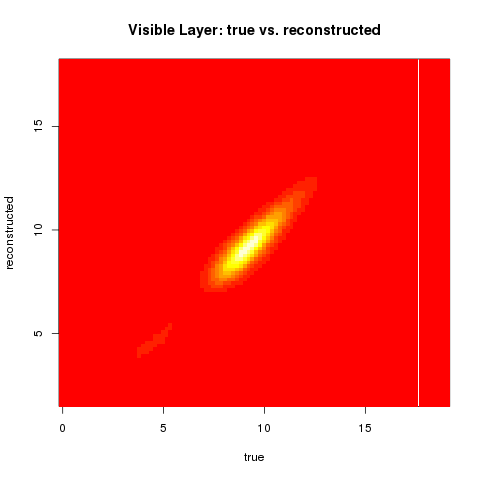
\includegraphics[width=0.3\columnwidth]{images/summer_school_2014-reconstruction-error-heatmap.pdf}~~\includegraphics[width=0.3\columnwidth]{images/summer_school_2014-reconstruction-error-boxplot.pdf}~~\includegraphics[width=0.3\columnwidth]{images/summer_school_2014-reconstruction-error-histogram.pdf}
\par\end{centering}
\caption[Rectionstruction error of data set breast\_cancer\_0.]{\label{fig:Reconstruction-error-breast_cancer_0}Rectionstruction
error of data set breast\_cancer\_0. Left: True (x-axis) versus reconstructed
(y-axis) expression values of data set breast\_cancer\_0. The heatmap
shows pixels from red over yellow to white. A pixel in red means zero
genes and the brighter a pixel is, the more genes there are in the
pixel's respective true and reconstructed expression value intervals.
Middle: Boxplot of reconstruction errors of the 10,000 most variable
genes. Right: Histogram of reconstruction errors of the 10,000 most
variable genes. Most genes have a low reconstruction error. Displayed
is the mean reconstruction error over all test samples.}
\end{figure}

Although the 10,000 numbers were compressed into only 50 numbers,
the mean reconstruction error of the 10,000 genes was only 0.563 (see
figure \ref{fig:Reconstruction-error-breast_cancer_0} middle). Considering
that the possible range (log2-intensities) of microarray values is
in the interval {[}0;16{]}, this is equivalent to a relative error
of 3.5\%. This demonstrated that RBMs are able to reduce dimensionality
of an expression data set while preserving most information.

\section{Prediction Quality From Labeled Samples\label{sec:breast_cancer_06-and-breast_cancer_07}}

\subsection{Increasing Number of Labeled Samples}

\index{breast_cancer_06@breast\_cancer\_06}The goal of data set breast\_cancer\_06
was to verify if basic training works. This was verified by testing
whether the classifier improves with an increasing amount of labeled
samples. Therefore we trained using all unlabeled samples, and defined
supervised learning data sets which have less and less labeled training
and test samples. Models were pre-trained using either an RBM or autoencoder
and fine-tuned with supervised back-propagation.

\paragraph{Definition of unlabeled data sets\label{par:Definition-of-unlabeled-data-sets-for-breast_cancer_06}}

A summary of unlabeled training, validation, and testing data sets
is shown in table \ref{tab:unlabeled-data-sets-of-breast_cancer_06}.
Validation samples were defined in case they were needed. Samples
from GSE17705 were included to give unsupervised training access to
more samples. (In later experiments, GSE17705 was left out to increase
the probability that samples are from the same distribution.)

\begin{table}
\begin{centering}
\begin{tabular}{|c|c|c||c|c||c||c|}
\hline 
 & GSE17705 & \multicolumn{2}{c|}{GSE25055} & \multicolumn{2}{c||}{GSE25065} & $\sum$\tabularnewline
\hline 
training & 239 & \multicolumn{2}{c|}{248} & \multicolumn{2}{c||}{159} & 646\tabularnewline
\hline 
validation & 29 & \multicolumn{2}{c|}{31} & \multicolumn{2}{c||}{19} & 79\tabularnewline
\hline 
testing & 30 & \multicolumn{2}{c|}{31} & \multicolumn{2}{c||}{20} & 81\tabularnewline
\hline 
\end{tabular}
\par\end{centering}
\caption{\label{tab:unlabeled-data-sets-of-breast_cancer_06}Sources of the
unlabeled data sets.}
\end{table}

\paragraph{Definition of labeled data sets}

To define the smaller and smaller labeled training data sets, we took
smaller and smaller fractions of the total 306 available labeled GSE25055
samples. The fractions were as displayed in table \ref{tab:training-and-validation-sets-of-breast_cancer_06}.

\noindent 
\begin{table}
\noindent \begin{centering}
\begin{tabular}{|c|c||c|c|c|c|c|c|c|}
\hline 
fraction & rep & \multicolumn{3}{c|}{training samples} & \multicolumn{3}{c|}{validation samples} & $\sum$\tabularnewline
\hline 
 &  & label 0 & label 1 & $\sum$ & label 0 & label 1 & $\sum$ & \tabularnewline
\hline 
\hline 
0.99 & 5 & 197 & 45 & 242 & 49 & 11 & 60 & 302\tabularnewline
\hline 
0.5 & 5 & 100 & 23 & 123 & 24 & 5 & 29 & 152\tabularnewline
\hline 
0.25 & 5 & 50 & 12 & 62 & 12 & 2 & 14 & 76\tabularnewline
\hline 
0.125 & 5 & 25 & 6 & 31 & 6 & 1 & 7 & 38\tabularnewline
\hline 
0.0625 & 5 & 12 & 3 & 15 & 3 & 0 & 3 & 18\tabularnewline
\hline 
\end{tabular}
\par\end{centering}
\caption[Sample distribution of training and validation sets of breast\_cancer\_06.]{\label{tab:training-and-validation-sets-of-breast_cancer_06}Sample
distribution of training and validation sets of data set breast\_cancer\_06.
The ``fraction'' in a data set denotes the fraction of the 306 labeled
samples GSE25055. The fraction of labeled samples used in a row is
split between training and validation data. Each of the 5 defined
data sets (rows) has 5 sub-sampled repetitions (``rep''), to be
able to draw error bars. Note that the number of samples is not balanced
between label 0 and label 1 samples.}
\end{table}

The testing set consists of all labeled GSE25065 samples, and no GSE25055
samples. (See table \ref{tab:Testing-set-for-breast_cancer_06}.)
Thus, betting on the largest group 0 yields an accuracy of $140/182\approx0.769$.

\noindent 
\begin{table}
\noindent \begin{centering}
\begin{tabular}{|c|c|c|c|c|c||c|}
\hline 
 & GSE17705 & \multicolumn{2}{c|}{GSE25055} & \multicolumn{2}{c||}{GSE25065} & \multirow{2}{*}{$\sum$}\tabularnewline
\cline{1-6} 
 &  & label 0 & label 1 & label 0 & label 1 & \tabularnewline
\hline 
\hline 
testing\_GSE25065 & 0 & 0 & 0 & 140 & 42 & 182\tabularnewline
\hline 
\end{tabular}
\par\end{centering}
\caption{\label{tab:Testing-set-for-breast_cancer_06}The testing set for data
set breast\_cancer\_06 consists of all labeled GSE25065 samples.}
\end{table}

In the next subsections, we describe the settings for pre-training
and fine-tuning.


\subsubsection{Unsupervised Pre-training Using RBM}

\index{breast_cancer_04_bg - bj@breast\_cancer\_04\_bg - bj}For unsupervised
pre-training of the RBM, we tried four different configurations that
are denoted in table \ref{tab:deepnet-settings-for-breast_cancer_04_bg-bj}.
(They were re-used from the runs labeled breast\_cancer\_04, which
are not described here.)

The reconstruction errors observed at the input layer during training
are shown in figure \ref{fig:reconstruction-errors-of-breast_cancer_04_bg-bj}.
In each training step, they (stochastically) decrease for all four
configurations and for training, validation, and testing data set.
Of note in this plot is that there is no overfitting since training
reconstruction error does not rise at the end of training. Also note
that the reconstruction error was not normalized to the number of
samples.

\begin{table}
\begin{centering}
\begin{tabular}{|c|c|c|c|c|}
\hline 
network instance & \_04\_bg & \_04\_bh & \_04\_bi & \_04\_bj\tabularnewline
\hline 
\hline 
network setting & value & value & value & value\tabularnewline
\hline 
\hline 
$base\textrm{\_}epsilon$ & 0.001 &  &  & \tabularnewline
\hline 
$activation$ & LOGISTIC &  &  & \tabularnewline
\hline 
$initial\textrm{\_}momentum$ & 0.5 &  &  & \tabularnewline
\hline 
$final\_momentum$ & 0.9 &  &  & \tabularnewline
\hline 
$momentum\textrm{\_}change\textrm{\_}steps$ & 3000 &  &  & \tabularnewline
\hline 
$sparsity$ & true &  &  & \tabularnewline
\hline 
$sparsity\textrm{\_}target$ & 0.5 & 0.5 & 0.25 & 0.1\tabularnewline
\hline 
$sparsity\textrm{\_}cost$ & 0.01 &  &  & \tabularnewline
\hline 
$sparsity\textrm{\_}damping$ & 0.9 &  &  & \tabularnewline
\hline 
$dropout$ & false &  &  & \tabularnewline
\hline 
$apply\textrm{\_}l2\textrm{\_}decay$ & true &  &  & \tabularnewline
\hline 
$l2\textrm{\_}decay$ & 0.001 &  &  & \tabularnewline
\hline 
\hline 
input layer setting & value & value & value & value\tabularnewline
\hline 
\hline 
$dimensions$ & 500 &  &  & \tabularnewline
\hline 
$sparsity$ & false &  &  & \tabularnewline
\hline 
\hline 
hidden layer 1 setting & value & value & value & value\tabularnewline
\hline 
\hline 
$dimensions$ & 500 & 1000 & 1000 & 1000\tabularnewline
\hline 
\end{tabular}
\par\end{centering}
\caption[\emph{deepnet }settings for unsupervised pre-training RBMs breast\_cancer\_04\_bg
- bj.]{\label{tab:deepnet-settings-for-breast_cancer_04_bg-bj}\emph{deepnet
}settings for unsupervised pre-training RBMs breast\_cancer\_04\_bg
- bj. No entry in a cell means that it has the same value as the cell
to the left.}
\end{table}

\begin{figure}
\begin{centering}
\includegraphics[width=0.35\columnwidth]{images/breast_cancer_04-plot-bg_bj}
\par\end{centering}
\caption[Reconstruction error of training, validation and testing data sets.]{\label{fig:reconstruction-errors-of-breast_cancer_04_bg-bj}Reconstruction
errors of training (T\_E), validation (V\_E) and testing (E\_E) data
sets for unsupervised training of an RBM with configurations breast\_cancer\_04\_bg,
bh, bi, bj. The y-axis is the reconstruction error, not normalized
for the number of samples, and the x-axis is the training step of
neural network training.}
\end{figure}

\subsubsection{Supervised Classification with Unsupervisedly Pre-trained RBM}

The settings for the supervised training runs \index{breast_cancer_06_aa - ad@breast\_cancer\_06\_aa - ad}breast\_cancer\_06\_aa
- ad were as described in table \ref{tab:deepnet-settings-for-breast_cancer_06_aa-ad}.
Four different models were tested, differing in number of nodes in
hidden layer 1 (setting $dimensions$) and the pre-trained weights
and biases between the input layer and hidden layer 1 (setting $pretrained\textrm{\_}model$).

\begin{table}
\begin{centering}
\begin{tabular}{|c|c|c|c|c|}
\hline 
network instance & \_06\_aa & \_06\_ab & \_06\_ac & \_06\_ad\tabularnewline
\hline 
\hline 
network setting & value & value & value & value\tabularnewline
\hline 
\hline 
$base\textrm{\_}epsilon$ & 0.001 &  &  & \tabularnewline
\hline 
$activation$ & LOGISTIC &  &  & \tabularnewline
\hline 
$initial\textrm{\_}momentum$ & 0.5 &  &  & \tabularnewline
\hline 
$final\_momentum$ & 0.9 &  &  & \tabularnewline
\hline 
$momentum\textrm{\_}change\textrm{\_}steps$ & 3000 &  &  & \tabularnewline
\hline 
$dropout$ & true &  &  & \tabularnewline
\hline 
$dropout\textrm{\_}prob$ & 0.5 &  &  & \tabularnewline
\hline 
$apply\textrm{\_}l2\textrm{\_}decay$ & true &  &  & \tabularnewline
\hline 
$l2\textrm{\_}decay$ & 0.001 &  &  & \tabularnewline
\hline 
\hline 
input layer setting & value & value & value & value\tabularnewline
\hline 
\hline 
$dimensions$ & 500 &  &  & \tabularnewline
\hline 
$dropout\textrm{\_}prob$ & 0.2 &  &  & \tabularnewline
\hline 
\hline 
hidden layer 1 setting & value & value & value & value\tabularnewline
\hline 
\hline 
$dimensions$ & 500 & 1000 & 1000 & 1000\tabularnewline
\hline 
$pretrained\textrm{\_}model$ & \_04\_bg & \_04\_bh & \_04\_bi & \_04\_bj\tabularnewline
\hline 
\hline 
output layer setting & value & value & value & value\tabularnewline
\hline 
\hline 
$dimensions$ & 1 &  &  & \tabularnewline
\hline 
$loss\textrm{\_}function$ & CROSS\_ENTROPY &  &  & \tabularnewline
\hline 
$activation$ & SOFTMAX &  &  & \tabularnewline
\hline 
$dropout$ & false &  &  & \tabularnewline
\hline 
\end{tabular}
\par\end{centering}
\caption[$deepnet$ settings for the classifiers breast\_cancer\_06\_aa - ad.]{\label{tab:deepnet-settings-for-breast_cancer_06_aa-ad}$deepnet$
settings for the classifiers breast\_cancer\_06\_aa - ad. Each classifier
is initialized using an unsupervisedly pre-trained RBM, and trained
supervisedly on data set breast\_cancer\_06. No entry in a cell means
that it has the same value as the cell to the left. The only difference
between the four configurations is the hidden layer 1 size ($dimensions$)
and initialization ($pretrained\textrm{\_}model$).}
\end{table}

For each of the $5$ differently sized training data sets, for each
of the $5$ repetitions, and for each of the $4$ differently pre-trained
RBMs, a classifier was trained. (So altogether $5*5*4=100$ classifiers
were trained.) Performance was then assessed through the accuracy,
as shown in figure \ref{fig:accuracy-plots-of-breast_cancer_06_aa-ad}.

\begin{figure}
\begin{centering}
\includegraphics[width=0.68\paperwidth]{images/breast_cancer_06-loess-aa_ad.pdf}
\par\end{centering}
\caption[Box plots showing the accuracies of the models breast\_cancer\_06\_aa
- ad.]{\label{fig:accuracy-plots-of-breast_cancer_06_aa-ad}Box plots showing
the accuracies of the models breast\_cancer\_06\_aa - ad. Each panel
shows one of the four configurations breast\_cancer\_06\_aa - ad.
In each panel, the x-axis shows the number of labeled samples in the
5 different data sets. The y-axis shows the smoothed accuracy, as
described in section \ref{subsec:Model-selection}. Each dot is the
accuracy of a repetition in the respective data set.}
\end{figure}

Surprisingly, the neural network accuracies do not improve with increasing
number of labeled samples. Instead it seems that the classifiers using
the least and most (18 and 302) samples perform best, and all others
(especially those using 76 samples) perform worst. As we will see,
this is due to an unbalanced number of label 0 and label 1 samples
in the training set. The tendency that the accuracies for 18 labeled
samples are about as high as those for 302 labeled samples, and are
the lower the closer the number of labeled samples are to 76 samples,
could be due to using the same pre-trained hidden-layer weights and
biases across the 5 repetitions. (The supervised training and validation
data are sampled independelty though.)

We also tried using 2 hidden layers instead of 1. This did not improve
accuracy.

\subsubsection{Unsupervised Pre-training Using Autoencoder\label{subsec:Unsupervised-pre-training-using-autoencoder}}

\index{breast_cancer_03_ai@breast\_cancer\_03\_ai}\index{breast_cancer_03_al@breast\_cancer\_03\_al}\index{breast_cancer_03_am@breast\_cancer\_03\_am}\index{breast_cancer_03_ao@breast\_cancer\_03\_ao}Settings
for unsupervised pre-training of the autoencoders are given in table
\ref{tab:deepnet-settings-for-breast_cancer_03_ai,_al,_am,_ao} (named
breast\_cancer\_03\_ai - am,ao). The only differences between the
models are in $base\mbox{\_}epsilon$ and $activation$.

\begin{table}
\begin{centering}
\begin{tabular}{|c|c|c|c|c|}
\hline 
network instance & \_03\_ai & \_03\_al & \_03\_am & \_03\_ao\tabularnewline
\hline 
\hline 
network setting & value & value & value & value\tabularnewline
\hline 
\hline 
$base\textrm{\_}epsilon$ & 1.0 & 0.01 & 0.01 & 0.1\tabularnewline
\hline 
$activation$ & LOGISTIC & RECTIFIED\_LINEAR & LOGISTIC & \tabularnewline
\hline 
$initial\textrm{\_}momentum$ & 0.5 &  &  & \tabularnewline
\hline 
$final\_momentum$ & 0.99 &  &  & \tabularnewline
\hline 
$momentum\textrm{\_}change\textrm{\_}steps$ & 50000 &  &  & \tabularnewline
\hline 
$dropout$ & true &  &  & \tabularnewline
\hline 
$dropout\textrm{\_}prob$ & 0.5 &  &  & \tabularnewline
\hline 
$apply\textrm{\_}l2\textrm{\_}decay$ & false &  &  & \tabularnewline
\hline 
$l2\textrm{\_}decay$ & 0.0001 &  &  & \tabularnewline
\hline 
\hline 
input layer setting & value & value & value & value\tabularnewline
\hline 
\hline 
$dimensions$ & 500 &  &  & \tabularnewline
\hline 
$dropout\textrm{\_}prob$ & 0.2 &  &  & \tabularnewline
\hline 
\hline 
hidden layer 1 setting & value & value & value & value\tabularnewline
\hline 
\hline 
$dimensions$ & 1000 &  &  & \tabularnewline
\hline 
\end{tabular}
\par\end{centering}
\caption[Settings for the unsupervised pre-training autoencoders breast\_cancer\_03\_ai,
\_03\_al, \_03\_am, and \_03\_ao.]{\label{tab:deepnet-settings-for-breast_cancer_03_ai,_al,_am,_ao}Settings
for the unsupervised pre-training autoencoders breast\_cancer\_03\_ai,
\_03\_al, \_03\_am, and \_03\_ao. No entry in a cell means that it
has the same value as the cell to the left.}
\end{table}

\subsubsection{Supervised Classification with Unsupervisedly Pre-trained Autoencoder}

\index{breast_cancer_06_ae - ah@breast\_cancer\_06\_ae - ah}When
training a neural network using back-propagation that was pre-trained
using one of the four autoencoders described in the previous section,
the resulting accuracy plots looked similar to the ones when pre-training
with an RBM (plots not shown). As we will see, similar to pre-training
using RBMs, this is due to an uneven number of label 0 and label 1
samples in the training set.

Like for RBMs, we also tried using 2 hidden layers instead of 1, but
this did not improve accuracy.

\subsubsection{High Label Prediction Bias\label{par:Examining-biased-classifier}}

\index{breast_cancer_06_aa/_n302_cv1@breast\_cancer\_06\_aa/\_n302\_cv1}The
lack of the accuracy increasing with the number of labeled training
samples can be explained by the following observation.

When examining the predictions of model breast\_cancer\_06\_aa/\_n302\_cv1
(the first network pre-trained on 302 samples), it becomes evident
that the training is sub-optimal, because label 0 is predicted almost
exclusively.  Table \ref{tab:predictions-of-breast_cancer_06_aa/_n302_cv1}
shows the predicted classes. 
\begin{table}
\begin{centering}
\begin{tabular}{|c|c|c|}
\hline 
 & label 0 & label 1\tabularnewline
\hline 
\hline 
training & 240 & 2\tabularnewline
\hline 
validation & 58 & 2\tabularnewline
\hline 
testing & 182 & 0\tabularnewline
\hline 
\end{tabular}
\par\end{centering}
\caption{\label{tab:predictions-of-breast_cancer_06_aa/_n302_cv1}Predictions
of the network breast\_cancer\_06\_aa/\_n302\_cv1.}
\end{table}

There is a heavy bias in favor of label 0. Our hypothesis was that
this is due to the unbalanced class label distribution in data set
breast\_cancer\_06. Therefore, the next data set is balanced in this
regard.

\subsection{Equal Number of Class Labels \label{subsec:Increasing-number-of-labeled-samples-and-equal-number-of-class-labels}}

As in the previous section on breast\_cancer\_06, in data set \index{breast_cancer_07@breast\_cancer\_07}breast\_cancer\_07,
we wanted to check whether the artificial neural networks accuracies
improve with an increasing number of labeled samples. Unlabeled data
sets were the same as for breast\_cancer\_06, see table \vref{tab:unlabeled-data-sets-of-breast_cancer_06}.
In contrast to the previous data set breast\_cancer\_06, each labeled
data set contains as many label 0 samples as label 1 samples (see
table \ref{tab:Data-set-breast_cancer_07}). The testing data set
is the same as in breast\_cancer\_06 and exclusively consists of GSE25065
samples, see table \vref{tab:Testing-set-for-breast_cancer_06}.

\begin{table}
\noindent \begin{centering}
\begin{tabular}{|c|c|c|c|c|c|c|c|c|}
\hline 
\multirow{2}{*}{data set} & \multirow{2}{*}{rep} & \multicolumn{3}{c|}{training samples} & \multicolumn{3}{c|}{validation samples} & \multirow{2}{*}{$\sum$}\tabularnewline
\cline{3-8} 
 &  & label 0 & label 1 & $\sum$ & label 0 & label 1 & $\sum$ & \tabularnewline
\hline 
\hline 
1 & 5 & 45 & 45 & 90 & 49 & 11 & 60 & 150\tabularnewline
\hline 
2 & 5 & 23 & 23 & 46 & 24 & 5 & 29 & 75\tabularnewline
\hline 
3 & 5 & 12 & 12 & 24 & 12 & 2 & 14 & 38\tabularnewline
\hline 
4 & 5 & 6 & 6 & 12 & 6 & 1 & 7 & 19\tabularnewline
\hline 
5 & 5 & 3 & 3 & 6 & 3 & 0 & 3 & 9\tabularnewline
\hline 
\end{tabular}
\par\end{centering}
\caption[Samples in data set breast\_cancer\_07.]{\label{tab:Data-set-breast_cancer_07}Samples in data set breast\_cancer\_07.
``rep'' is the number of subsamplings from all samples described
by a line in the table. Note that there is an equal number of training
samples for each class, but an unequal number in the validation data
sets.}
\end{table}

Only the 500 most variable genes were used. The training and validation
data sets were generated from subsets of GSE25055. Each training data
set had an equal number of samples from class 0 and class 1. However,
the validation data sets contained a larger number of class 0 samples,
because there were only 57 label 1 samples in GSE25055, and 45 of
them were needed for training. The test data set is composed of all
GSE25065 samples. Each data set was drawn 5 times from the samples
as described for training and validation data set. This is to repeat
the experiment 5 times and to be able to obtain error bars for the
accuracies.

If we were to bet on the larger test set class we would achieve an
accuracy of $140/182=0.769$, because the test set contains 140 label
0 samples, but only 42 label 1 samples. However, because the training
data set contains an equal number of label 0 and label 1 samples,
the test set accuracy should not be as biased as data set breast\_cancer\_06,
whose training data set is imbalanced.

The following machine learning algorithms were tested on this data
set: SVM, TSVM, supervised classification with unsupervised pre-trained
RBM, supervised classification with unsupervisedly pre-trained autoencoder,
supervised classification without pre-training. Unsupervised pre-training
was performed as for breast\_cancer\_06.

\subsubsection{SVM Accuracies}

\begin{figure}
\begin{centering}
\includegraphics[width=0.34\paperwidth]{images/breast_cancer_07-accuracies-svm-testing.pdf}
\par\end{centering}
\caption[Accuracy box plots of SVM predicting data set breast\_cancer\_07.]{\label{fig:Accuracy-box-plots-of-SVM-on-breast_cancer_07}Accuracy
box plots of SVM predicting the testing data of breast\_cancer\_07.
On the x-axis are the sizes of the data sets containing an increasing
number of labeled samples. On the y-axis are the accuracies obtained
on the testing data.}
\end{figure}

Figure \ref{fig:Accuracy-box-plots-of-SVM-on-breast_cancer_07} shows
there is the tendency that adding more samples to supervised learning
yields better accuracy. Although the 25\%- and 75\%-quantile of the
boxplots suggest different variances, we believe that the boxplots
should not be over-interpreted, as there are only 5 data points (5
subsamplings).

\subsubsection{TSVM Accuracies}

TSVM can utilize incomplete and unlabelled data to improve supervised
classification (``transductive SVM''). Figure \ref{fig:Accuracy-box-plots-of-TSVM-on-breast_cancer_07}
shows that TSVM sometimes fails to learn a model for the data sets
with less than 46 labeled samples and otherwise performs similarly
to a normal SVM.

\begin{figure}
\begin{centering}
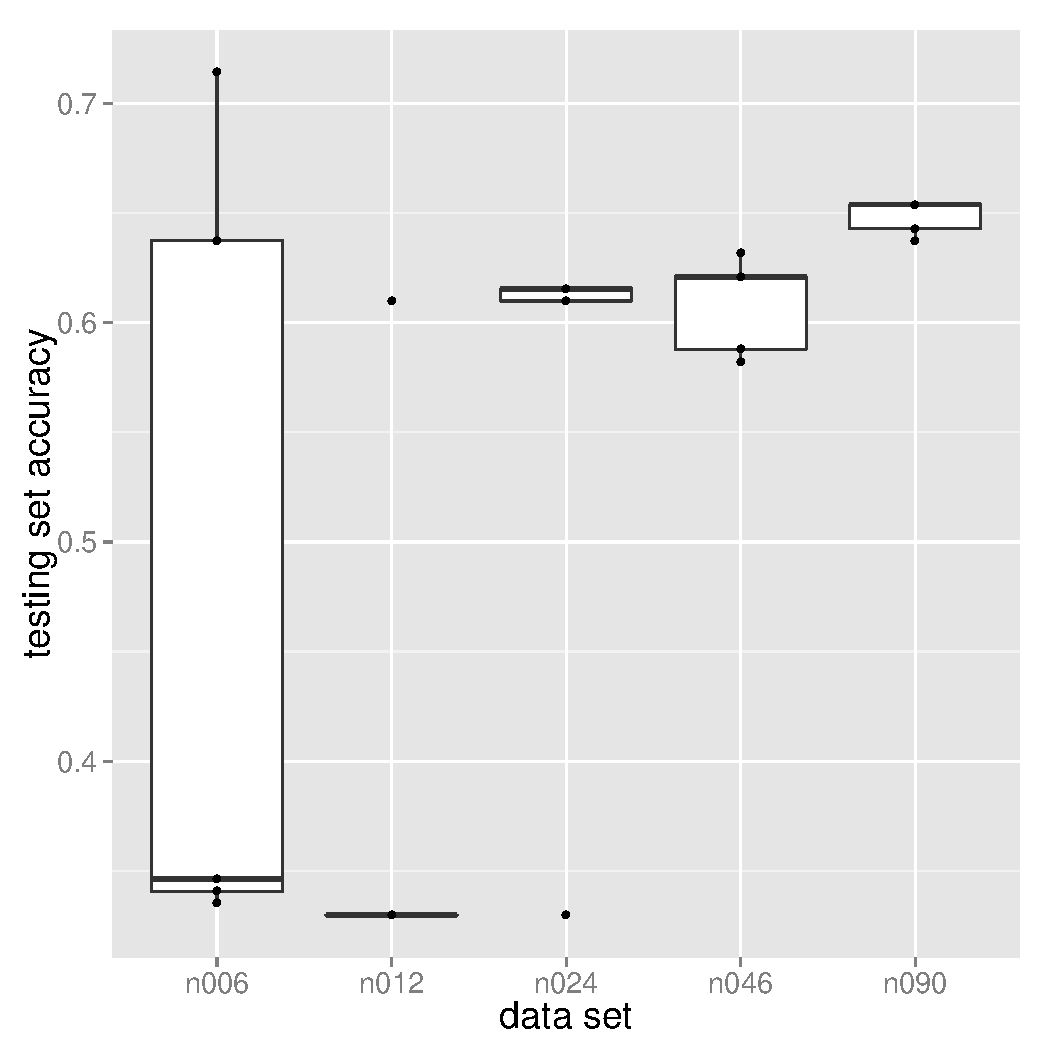
\includegraphics[width=0.34\paperwidth]{images/breast_cancer_07-accuracies-svmlight.pdf}
\par\end{centering}
\caption[Accuracy box plots of TSVM predicting data set of breast\_cancer\_07.]{\label{fig:Accuracy-box-plots-of-TSVM-on-breast_cancer_07}Accuracy
box plots of TSVM predicting the testing data set of breast\_cancer\_07.
On the x-axis are the sizes of the data sets containing an increasing
number of labeled samples. On the y-axis are the accuracies obtained
on the testing data.}
\end{figure}

\subsubsection{Supervised Classification with Unsupervisedly Pre-trained RBM}

The \emph{deepnet }settings for training runs \index{breast_cancer_07_aa - ad@breast\_cancer\_07\_aa - ad}breast\_cancer\_07\_aa
- ad were the same as those for breast\_cancer\_06\_aa - ad (see table
\vref{tab:deepnet-settings-for-breast_cancer_06_aa-ad}).

As expected, the accuracy plots in figure \ref{fig:Accuracy-box-plots-of-breast_cancer_07_aa-ad}
show that all 4 neural networks perform better the more labeled samples
there are in training. In addition the variance of the accuracies
decreases, the more labeled samples there are in training.

\begin{figure}
\begin{centering}
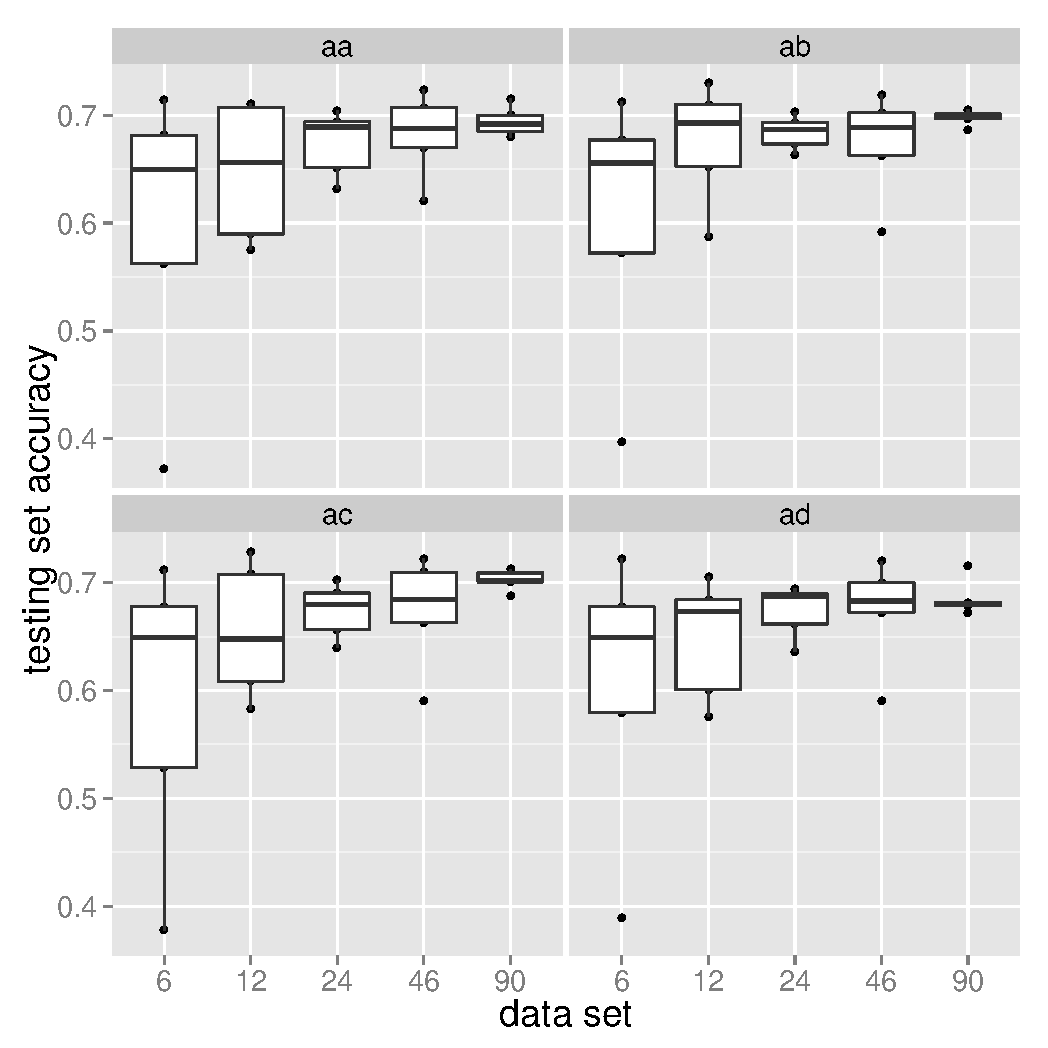
\includegraphics[width=0.68\paperwidth]{images/breast_cancer_07-accuracies-aa_ad.pdf}
\par\end{centering}
\caption[Accuracy box plots of a feed-forward neural network pre-trained with
an RBM, predicting the testing data set of breast\_cancer\_07.]{\label{fig:Accuracy-box-plots-of-breast_cancer_07_aa-ad}Accuracy
box plots of a feed-forward neural network pre-trained with an RBM,
predicting the testing data set of breast\_cancer\_07. On the x-axis
are the sizes of the data sets containing an increasing number of
labeled samples. On the y-axis are the accuracies obtained on the
testing data.}
\end{figure}

\subsubsection{Supervised Classification with Unsupervisedly Pre-trained Autoencoder}

The settings for \emph{deepnet }training of \index{breast_cancer_07_ae - ah@breast\_cancer\_07\_ae - ah}breast\_cancer\_07\_ae
- ah were as those for breast\_cancer\_06\_ae - ah. As is shown in
figure \ref{fig:Accuracy-box-plots-of-breast_cancer_07_ae-ah}, pre-training
with an autoencoder yields similar accuracies as pre-training with
an RBM.

\begin{figure}
\begin{centering}
\includegraphics[width=0.68\paperwidth]{images/breast_cancer_07-accuracies-ae_ah.pdf}
\par\end{centering}
\caption[Accuracy box plots of a feed-forward neural network pre-trained with
an autoencoder, predicting the testing data set of breast\_cancer\_07.]{\label{fig:Accuracy-box-plots-of-breast_cancer_07_ae-ah}Accuracy
box plots of a feed-forward neural network pre-trained with an autoencoder,
predicting the testing data set of breast\_cancer\_07. On the x-axis
are the sizes of the data sets containing an increasing number of
labeled samples. On the y-axis are the accuracies obtained on the
testing data.}
\end{figure}

\subsubsection{Supervised Classification without Pre-training}

Finally, in \index{breast_cancer_07_ai - aj@breast\_cancer\_07\_ai - aj}breast\_cancer\_07\_ai
- aj, we trained the neural networks with no pre-training at all,
but using only back-propagation. The \emph{deepnet} settings are shown
in table \ref{tab:deepnet-settings-for-breast_cancer_07_ai-aj}.

\begin{table}
\begin{centering}
\begin{tabular}{|c|c|c|}
\hline 
network instance & \_07\_ai & \_07\_aj\tabularnewline
\hline 
\hline 
network setting & value & value\tabularnewline
\hline 
\hline 
$base\textrm{\_}epsilon$ & 0.001 & \tabularnewline
\hline 
$activation$ & LOGISTIC & \tabularnewline
\hline 
$initial\textrm{\_}momentum$ & 0.5 & \tabularnewline
\hline 
$final\_momentum$ & 0.9 & \tabularnewline
\hline 
$momentum\textrm{\_}change\textrm{\_}steps$ & 3000 & \tabularnewline
\hline 
$dropout$ & true & false\tabularnewline
\hline 
$dropout\textrm{\_}prob$ & 0.5 & \tabularnewline
\hline 
$apply\textrm{\_}l2\textrm{\_}decay$ & true & \tabularnewline
\hline 
$l2\textrm{\_}decay$ & 0.001 & \tabularnewline
\hline 
\hline 
input layer setting & value & value\tabularnewline
\hline 
\hline 
$dimensions$ & 500 & \tabularnewline
\hline 
$dropout\textrm{\_}prob$ & 0.2 & \tabularnewline
\hline 
\hline 
hidden layer 1 setting & value & value\tabularnewline
\hline 
\hline 
$dimensions$ & 1000 & \tabularnewline
\hline 
$initialization$ & CONSTANT & \tabularnewline
\hline 
\hline 
output layer setting & value & value\tabularnewline
\hline 
\hline 
$dimensions$ & 1 & \tabularnewline
\hline 
$loss\textrm{\_}function$ & CROSS\_ENTROPY & \tabularnewline
\hline 
$activation$ & SOFTMAX & \tabularnewline
\hline 
$dropout$ & false & \tabularnewline
\hline 
\end{tabular}
\par\end{centering}
\caption[Settings for the classifiers breast\_cancer\_07\_ai - aj.]{\label{tab:deepnet-settings-for-breast_cancer_07_ai-aj}Settings
for the classifiers breast\_cancer\_07\_ai - aj, which is trained
using backpropagation only (without pre-training). Each classifier
is trained supervisedly on data set breast\_cancer\_07. The only difference
between the two configurations is the use of $dropout$ in breast\_cancer\_07\_ai.
No entry in a cell means that it has the same value as the cell to
the left.}
\end{table}

\begin{figure}
\begin{centering}
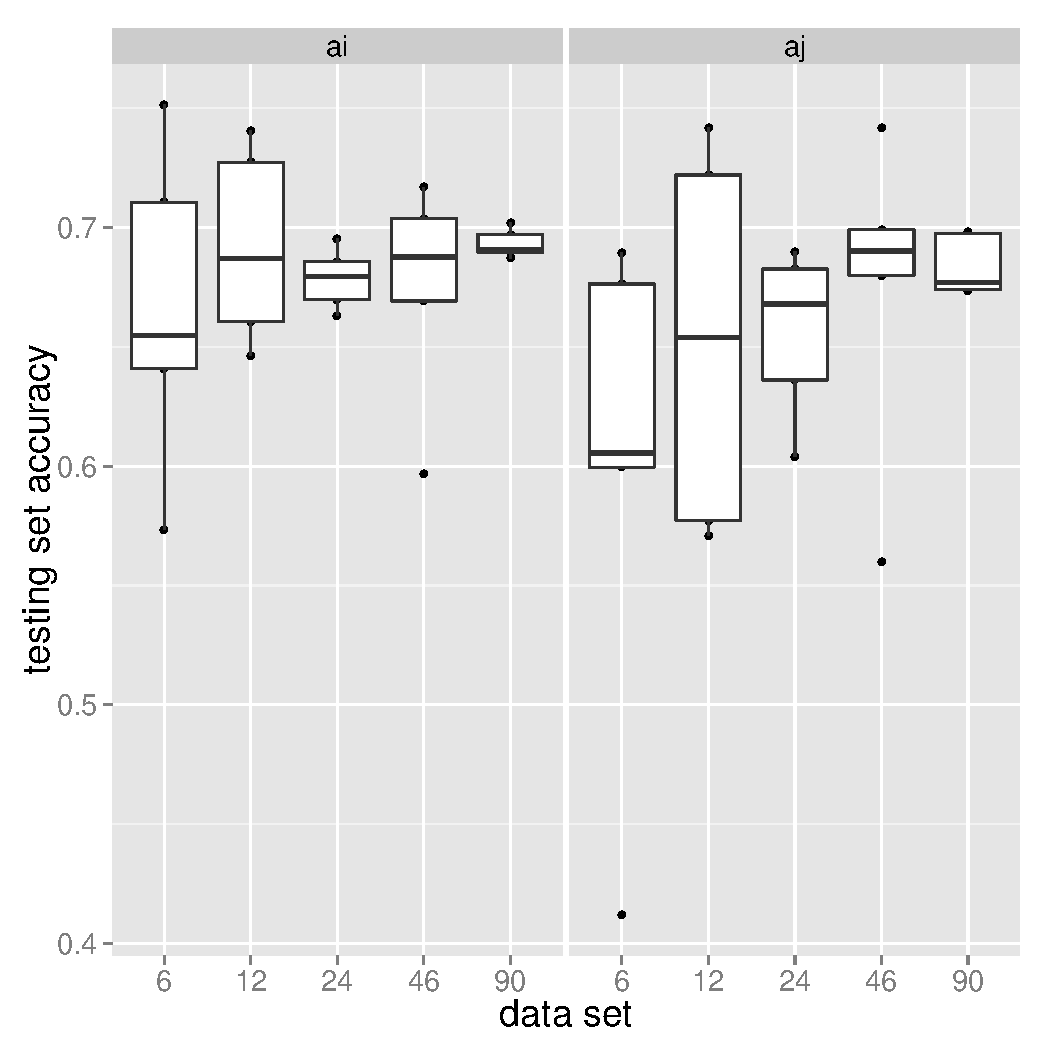
\includegraphics[width=0.68\paperwidth]{images/breast_cancer_07-accuracies-ai_aj.pdf}
\par\end{centering}
\caption[Accuracy box plots of feed-forward neural networks not pre-trained,
predicting the testing data set of breast\_cancer\_07.]{\label{fig:Accuracy-box-plots-of-breast_cancer_07_ai-aj}Accuracy
box plots of feed-forward neural networks not pre-trained, predicting
the testing data set of breast\_cancer\_07. On the x-axis are the
sizes of the data sets containing an increasing number of labeled
samples. On the y-axis are the accuracies obtained on the testing
data. The panel ``ai'' stands for the classifier ``breast\_cancer\_07\_ai'',
``aj'' for ``breast\_cancer\_07\_aj''.}
\end{figure}

The accuracy plots are shown in figure \ref{fig:Accuracy-box-plots-of-breast_cancer_07_ai-aj}.
As can be seen, using $dropout$ (breast\_cancer\_07\_ai) yields better
accuracies than not using it (breast\_cancer\_07\_aj). An explanation
can be that \emph{$dropout$} reduces overfitting. In addition, comparing
with the neural networks pre-trained using RBM or autoencoder (e.g.
breast\_cancer\_07\_ai versus breast\_cancer\_07\_ag) might indicate
a slight advantage of not using pre-training (but using $dropout$)
in the data sets with little labeled samples. However, this assertion
should be re-done with more than 5 repetitions.

The accuracies of the classifiers on breast\_cancer\_07 are lower
than those on breast\_cancer\_06. This indicates the higher difficulty
of the classification task when the labels are balanced. We will look
into this in the following.

\subsubsection{Confusion Table of Predicted Classes}

Like for breast\_cancer\_06, we looked at the output of one of the
neuronal networks trained on data set breast\_cancer\_07. As can be
seen in table \ref{tab:predictions-of-breast_cancer_07_aa} and in
contrast to the predictions on data set breast\_cancer\_06, the predicted
classes are now more balanced.

\begin{table}
\begin{centering}
\begin{tabular}{|c|c|c|}
\hline 
 & label 0 & label 1\tabularnewline
\hline 
\hline 
training & 44 & 46\tabularnewline
\hline 
validation & 38 & 22\tabularnewline
\hline 
testing & 117 & 65\tabularnewline
\hline 
\end{tabular}
\par\end{centering}
\caption{\label{tab:predictions-of-breast_cancer_07_aa}Labels predicted by
\index{breast_cancer_07_aa/_n090_cv1@breast\_cancer\_07\_aa/\_n090\_cv1}breast\_cancer\_07\_aa/\_n090\_cv1
on training, validation, and testing data set.}
\end{table}

\paragraph{Confusion table on the test set samples}

\begin{table}
\begin{centering}
\begin{tabular}{|c||c|c|}
\hline 
 & true label 0 & true label 1\tabularnewline
\hline 
\hline 
predicted label 0 & 101 & 16\tabularnewline
\hline 
predicted label 1 & 39 & 26\tabularnewline
\hline 
\end{tabular}
\par\end{centering}
\caption[Confusion table of the predictions made by breast\_cancer\_07\_aa/\_n090.]{\label{tab:Confusion-table-of-breast_cancer_07_aa/_n090_cv1}Confusion
table of the predictions made by breast\_cancer\_07\_aa/\_n090\_cv1
(which was trained on 90 labeled samples) on the testing data set
of data set breast\_cancer\_07.}
\end{table}

The confusion table \ref{tab:Confusion-table-of-breast_cancer_07_aa/_n090_cv1}
shows the predicted and true labels in the testing data set. It shows
that most predicted label 1 samples are actually label 0 samples ($\frac{39}{39+26}$).
Of the true label 0 samples, $\frac{101}{101+39}\approx0.72$ are
classified correctly, and $\frac{26}{26+16}\approx0.62$ of the true
label 1 samples. This may indicate that predicting label 1 samples,
which means ``pathologic complete response'', i.e. no remaining
breast cancer, is more difficult than predicting ``residual disease''.

The predicted probabilities of the true class of the mis-classified
samples (i.e. those not on the main diagonal) can be displayed in
a histogram, see figure \ref{fig:Histogram-of-probabilities-of-breast_cancer_07}.
The histogram shows that the probabilities for the true class of mis-classified
samples are not mostly near 0.5, but in the middle of the possible
range. 0.5 is the maximum probability, otherwise the sample would
not be mis-classified.

\begin{figure}
\begin{centering}
\includegraphics[width=0.68\columnwidth]{images/breast_cancer_07-true-label-probabilities-of-misclassified-samples.pdf}
\par\end{centering}
\caption[Histogram of probabilities of samples predicted wrongly.]{\label{fig:Histogram-of-probabilities-of-breast_cancer_07}Histogram
of probabilities of samples predicted wrongly by breast\_cancer\_07\_aa/\_n090\_cv1.
The x-axis is the predicted probability of the true class; the y-axis
the counts of samples.}
\end{figure}

\section{Different Normalizations\label{sec:breast_cancer_08}}

One of the goals of this work was to show that adding unlabeled samples
increases accuracy in semi-supervised classification. To achieve that
goal, in \index{breast_cancer_08@breast\_cancer\_08}breast\_cancer\_08,
we built data sets with a constant number of labeled samples and an
increasing number of unlabeled samples.

To alleviate the effects of systematic errors in the raw data, we
tried different normalizations in order to search for normalizations
that are beneficial to classification accuracy. We assessed the effect
of different normalizations on unsupervised pre-training using an
autoencoder and supervised classification accuracy.

\subsection{Data Set Design}

Table \ref{tab:design-of-breast_cancer_08} shows the assignment of
samples to data sets. Note that labeled training and validation data
are almost exclusively from GSE25055, and labeled testing data are
exclusively from GSE25065.

Labeled training and testing data are balanced with respect to the
number of label 0 and label 1 samples. An unbalanced data set leads
to a biased classifier which prefers the label it was shown more often
during training. (As was demonstrated on page \pageref{par:Examining-biased-classifier}.)
The increasing number of unlabeled training data are mostly from GSE25055,
except data set 4, which also has unlabeled data from GSE25065. The
unlabeled training data are balanced in data sets 1 and 2, and in
proportions 1:2 and 1:4 in data sets 3 and 4, respectively.

\begin{table}
\begin{centering}
\begin{tabular}{|c|c||c|c|c|c|}
\hline 
 & data source & data set 1 & data set 2 & data set 3 & data set 4\tabularnewline
\hline 
\hline 
labeled training & GSE25055 & 28\textbar{}28 & 28\textbar{}28 & 28\textbar{}28 & 28\textbar{}28\tabularnewline
\hline 
\multirow{2}{*}{unlabeled training} & GSE25055 & 15\textbar{}15 & 29\textbar{}29 & 58\textbar{}29 & 58\textbar{}29\tabularnewline
\cline{2-6} 
 & GSE25065 & 0\textbar{}0 & 0\textbar{}0 & 0\textbar{}0 & 58\textbar{}0\tabularnewline
\hline 
\multirow{2}{*}{labeled validation} & GSE25055 & 221\textbar{}29 & 221\textbar{}29 & 221\textbar{}29 & 221\textbar{}29\tabularnewline
\cline{2-6} 
 & GSE25065 & 0\textbar{}0 & 0\textbar{}0 & 0\textbar{}0 & 0\textbar{}0\tabularnewline
\hline 
labeled testing & GSE25065 & 42\textbar{}42 & 42\textbar{}42 & 42\textbar{}42 & 42\textbar{}42\tabularnewline
\hline 
repeats &  & 5 & 5 & 5 & 5\tabularnewline
\hline 
proportions 0:1 &  & 1:1 & 1:1 & 2:1 & 4:1\tabularnewline
\hline 
\end{tabular}
\par\end{centering}
\caption[The design of data set breast\_cancer\_08.]{\label{tab:design-of-breast_cancer_08}The design of data set breast\_cancer\_08.
There are 4 sub-data-sets that have a constant number of labeled training,
labeled validation, and labeled testing samples. The unlabeled data
sets have an increasing number of samples. The syntax ``$x$\textbar{}$y$''
in a table cell means that there are $x$ samples having label 0,
and $y$ samples having label 1. The row ``repeats'' means that
each data set was created 5 times, by random sampling. The row ``proportions
0:1'' describes the relative proportions of label 0 and label 1 samples
in the ``unlabeled training'' rows.}
\end{table}

\pagebreak{}

\subsection{Normalizations}

We used RMA \cite{BolstadSpeed2003}, MAS5 \cite{Affymetrix2001},
MAS5+log2, RMA+ComBat, MAS5+ComBat, and MAS5+log2+ComBat to normalize
the raw microarray data (for ComBat, see \cite{JohnsonRabinovic2007}).
Because MAS5 does not logarithmize the data, but RMA does, MAS5 was
tried with additional logarithmizing of the data. ComBat was designed
as a batch-effect correction method. It produces a data set with the
same size as the original one, but with batch-effects between samples
removed. As input, ComBat needs the expression matrix and, for each
sample, the batch. We defined samples from the two sources GSE25055
and GSE25065 as batches. Table \ref{tab:normalizations-for-breast_cancer_08}
shows a list of different normalizations.

\begin{table}
\begin{centering}
\begin{tabular}{|c|c|c|}
\hline 
configuration & normalization & normalizations applied\tabularnewline
\hline 
\hline 
breast\_cancer\_08\_bb - bx & rma & RMA\tabularnewline
\hline 
breast\_cancer\_08\_by - cu & mas5 & MAS5\tabularnewline
\hline 
breast\_cancer\_08\_ep - fl & rma,combat & RMA, ComBat batch effect correction\tabularnewline
\hline 
breast\_cancer\_08\_fm - gi & mas5,combat & MAS5, ComBat batch effect correction\tabularnewline
\hline 
\end{tabular}
\par\end{centering}
\caption{\label{tab:normalizations-for-breast_cancer_08}Data set normalizations
tested in breast\_cancer\_08.}
\end{table}

For each of 4 different normalization pre-processing combinations,
we created each of the 4 data sets by random sampling from the designated
samples described in table \ref{tab:design-of-breast_cancer_08}.
The normalization steps were done in this order: first RMA/MAS5 normalization
and summarization (to default HG\_U133A probe sets), then ComBat (if
enabled), then splitting of the data matrices into the sub-data-sets
according to table \ref{tab:design-of-breast_cancer_08}.

\begin{table}
\begin{centering}
\begin{tabular}{|c||c|c|c|c|}
\hline 
\multirow{2}{*}{normalization} & \multicolumn{4}{c|}{data set}\tabularnewline
\cline{2-5} 
 & 1 & 2 & 3 & 4\tabularnewline
\hline 
\hline 
rma & 0.23 (.0032) & 0.41 (.0075) & 0.61 (.0061) & 1.02 (.016)\tabularnewline
\hline 
mas5 & 0.045 (.0022) & 0.053 (.00041) & 0.058 (.002) & 0.068 (.0029)\tabularnewline
\hline 
rma,combat & 0.24 (.0038) & 0.4 (.0028) & 0.6 (.0052) & 1.02 (.016)\tabularnewline
\hline 
mas5,combat & 0.057 (.0035) & 0.07 (.0011) & 0.079 (.0033) & 0.088 (.0034)\tabularnewline
\hline 
\end{tabular}
\par\end{centering}
\caption[Reconstruction error for differently normalized data.]{\label{tab:Reconstruction-error-for-breast_cancer_08}Reconstruction
error for differently normalized data. In the rows are the different
normalizations, and in the columns the data sets. Each cell in the
table contains the mean (and standard deviation in brackets) of the
reconstruction error over all repeats. The numbers are rounded to
two significant digits. Reconstruction errors shown for MAS5 were
computed on not logarithmized data.}
\end{table}

\subsection{Unsupervised Reconstruction Error in Autoencoder Pre-training}

Before looking at the accuracies of the supervised classifier, we
looked at unsupervised pre-training using an autoencoder. The reconstruction
error for each normalization is shown in table \ref{tab:Reconstruction-error-for-breast_cancer_08}.
Of note in this table are the following:
\begin{itemize}
\item The reconstruction error increases the more unlabeled data there are.
\item The MAS5 normalizations all have lower reconstruction errors than
their RMA counterpart with same concomitant normalization steps (vertically
alternating high and low mean).

\begin{itemize}
\item The standard deviation of the reconstruction errors across replicates
(i.e. with different unlabeled data) is consistently smaller for MAS5
than for RMA.
\end{itemize}
\item Additional ComBat batch effect correction does not improve the reconstruction
error of RMA or MAS5 normalized data.

\begin{itemize}
\item There is no clear trend in the table above how ComBat influences standard
deviation (across replications) of reconstruction errors.
\end{itemize}
\end{itemize}
Although it may seem beneficial to achieve reconstruction error as
a low as possible, we will see that a better (lower) reconstruction
error does not necessarily translate into a better (higher) accuracy.

After pre-training, the artificial neural networks were fine-tuned
using backpropagation and their accuracy to predict chemotherapy efficacy
was measured.

\subsection{Supervised Classification with Unsupervised Pre-trained Autoencoder}

\begin{figure}
\begin{centering}
\begin{tabular}{cc}
rma-data.pbtxt & mas5-data.pbtxt\tabularnewline
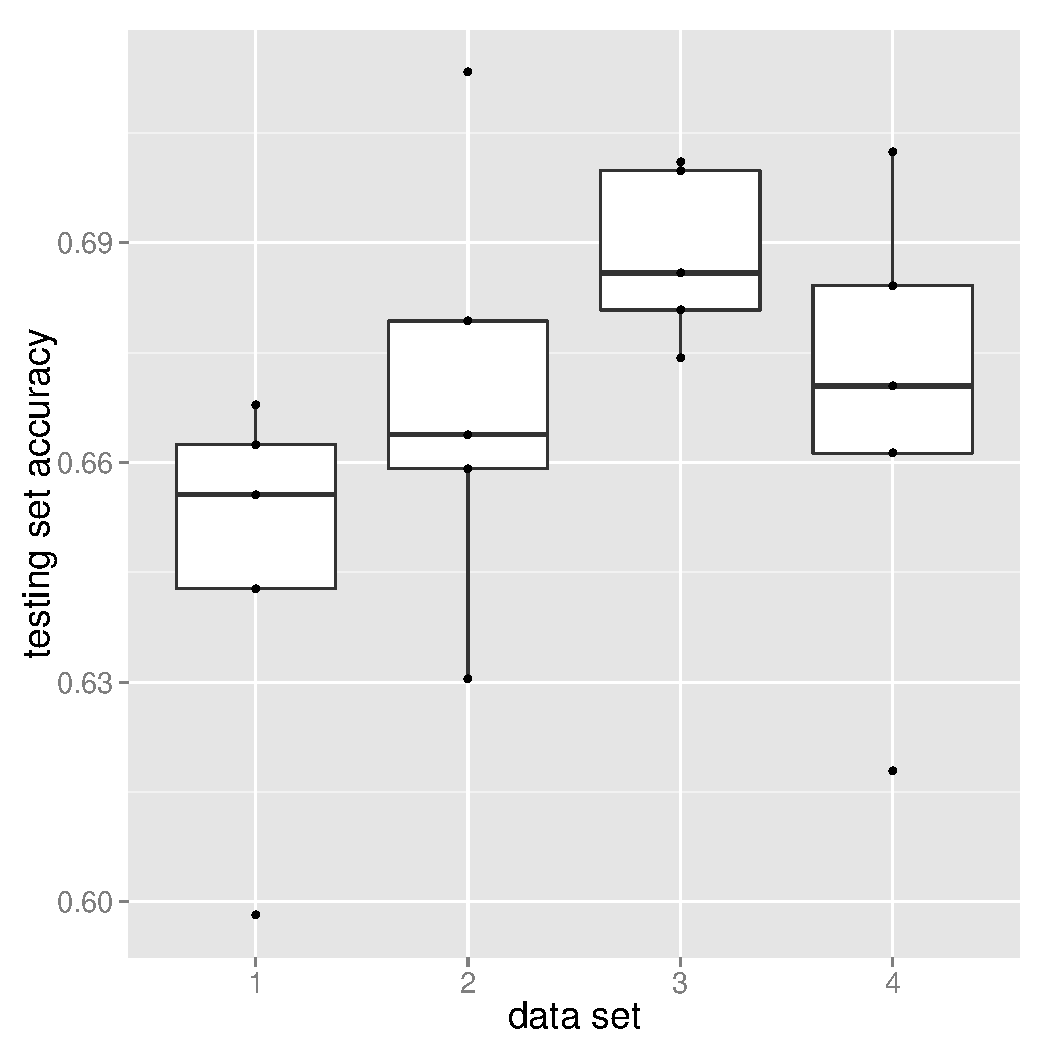
\includegraphics[width=0.34\paperwidth]{images/breast_cancer_08-accuracies-testing-bb_bu.pdf} & \includegraphics[width=0.34\paperwidth]{images/breast_cancer_08-accuracies-testing-by_cr.pdf}\tabularnewline
rma\_combat-data.pbtxt & mas5\_combat-data.pbtxt\tabularnewline
\includegraphics[width=0.34\paperwidth]{images/breast_cancer_08-accuracies-testing-ep_fi.pdf} & \includegraphics[width=0.34\paperwidth]{images/breast_cancer_08-accuracies-testing-fm_gf.pdf}\tabularnewline
\end{tabular}
\par\end{centering}
\caption[Box-plot for neural network prediction pre-trained with an autoencoder
on differently normalized data sets.]{\label{fig:accuracy-plots-for-breast_cancer_08}Box-plot for neural
network prediction pre-trained with an autoencoder on the 4 differently
normalized data sets rma-data.pbtxt, mas5-data.pbtxt, rma\_combat-data.pbtxt,
and mas5\_combat-data.pbtxt in breast\_cancer\_08. The box-plot shows
on the x-axis the 4 data sets, and on the y-axis the achieved accuracies
on the testing data set for each of the 5 repetitions.}
\end{figure}
The architecture of the classifier network was 500-1000-1. Figure
\ref{fig:accuracy-plots-for-breast_cancer_08} shows the resulting
accuracy box plots for the different normalizations. None of the plots
show a clear increasing accuracy from data set 1 to data set 4. However,
the silhouettes of the box-plots seem to show increasing accuracy.
``Silhouette'' means, for each data set, the interval from the accuracy
of the repetition with lowest to the accuracy of the repetition with
highest accuracy; or differently, the maximal outliers. In addition,
the median of the accuracies of data set 1 is smaller than the median
of the accuracies of both data set 3 and 4, for every normalization.
The fact that the median of the accuracies of data set 2 is not always
greater than the median of the accuracies of data set 1 could be due
to randomness in data subsampling when creating the 5 repetitions.
Another reason could be that the 28 additional unlabeled samples ($29-15=14$
label 0 samples, and 14 label 1 samples) provide little benefit to
a pre-trained classifier.

\subsubsection{Different Normalizations}

When comparing the accuracies yielded by the different normalizations
to each other, a table of the mean accuracies for each normalization
and data sets 1-4 is helpful. Table \ref{tab:Mean-accuracies-for-each-normalization}
shows the following:

\begin{table}
\begin{centering}
\begin{tabular}{|c||c|c|c|c|}
\hline 
normalization & \multicolumn{4}{c|}{data set}\tabularnewline
\hline 
 & 1 & 2 & 3 & 4\tabularnewline
\hline 
\hline 
rma & 0.65 & 0.67 & 0.69 & 0.67\tabularnewline
\hline 
mas5 & 0.58 & 0.58 & 0.63 & 0.61\tabularnewline
\hline 
mas5,log2 & 0.59 & 0.61 & 0.6 & 0.62\tabularnewline
\hline 
rma,combat & 0.61 & 0.61 & 0.62 & 0.61\tabularnewline
\hline 
mas5,combat & 0.60 & 0.59 & 0.63 & 0.64\tabularnewline
\hline 
mas5,log2,combat & 0.64 & 0.66 & 0.64 & 0.64\tabularnewline
\hline 
\end{tabular}
\par\end{centering}
\caption{\label{tab:Mean-accuracies-for-each-normalization}Mean accuracies
for each normalization and data set in breast\_cancer\_08.}
\end{table}
\begin{itemize}
\item RMA alone (i.e. without ComBat pre-processing) out-performs all other
tested combinations of normalization method and pre-processing in
all data sets tested.
\item Using ComBat as pre-processing leads to worse accuracies on the RMA-normalized
data, but improves accuracies when using MAS5 (except in data set
3).
\item RMA seems to perform consistently better than MAS5 without log2 (an
exception is data set 3 with ComBat pre-processing), but MAS5 with
log2 and ComBat perform better than RMA with ComBat (due to RMA taking
a performance hit when used together with ComBat).
\item Taking the log2 of MAS5-normalized data only improves accuracies when
the data is ComBat pre-processed.
\end{itemize}

\subsubsection{ZCA Normalization}

We also tried applying ZCA normalization after all 4 normalizations
tried above. This step helped in face recognition, for example \cite{KrizhevskyHinton2009}.
However, for our data set it resulted in random classifiers, i.e.
their accuracies were around 0.5.


\section{Comparison of SVM, TSVM, FFN, DBN\label{sec:breast_cancer_12}}

A problem in the design of the data sets of breast\_cancer\_08 is
that the number of label 0 and label 1 samples is not balanced. This
is due to the class imbalance in GSE25055 and GSE25065. The next data
set \index{breast_cancer_12@breast\_cancer\_12}breast\_cancer\_12
thus had balanced classes in the unlabeled training samples.

To be able to statistically detect a possible rise in accuracy with
a rising number of unlabeled samples, we also increased the number
of sub-sampling repetitions. Also, instead of using autoencoder or
RBM for pre-training, we used a Deep Belief Network.

\subsection{Data Set Design}

Following the same arguments as in creating data set breast\_cancer\_08,
we aimed for the following properties. All training/validation data
sets should have an equal number of 0/1 samples, otherwise \emph{deepnet}'s
predictions are biased towards the larger group. Samples used in the
unlabeled training/validation data set were also used for labeled
training/validation, otherwise there are not enough samples. Unlabeled
validation data sets were defined to be able to do model selection
during unsupervised training. As before, performance was measured
on the unseen test data sets.

There are the following differences between breast\_cancer\_12 and
breast\_cancer\_08. breast\_cancer\_12 includes an unlabeled validation
data set whose purpose is to be able to early-stop pre-training, which
was necessary for learning multiple hidden layers in a DBN. The only
normalization used was RMA (without ComBat), because it performed
best in data set breast\_cancer\_08. There are 20 instead of 5 repetitions
for each data set. Again the sub-sampling repetitions were made by
selecting the samples at random from the eligible samples. The labeled
samples were held constant across all 6 data sets within one repetition,
to be able to directly compare performance between e.g. data sets
1 and 3 within a repetition. The only difference between data sets
1 and 3 is the unlabeled pre-training data.

\begin{table}
\begin{centering}
\begin{tabular}{|c|c|c||c|c|c|c|c|c|}
\hline 
\multicolumn{3}{|c||}{data set} & 1 & 2 & 3 & 4 & 5 & 6\tabularnewline
\hline 
\hline 
\multirow{2}{*}{(labeled)} & \multirow{2}{*}{testing} & GSE25055 & 0\textbar{}0 & 0\textbar{}0 & 0\textbar{}0 & 0\textbar{}0 & 0\textbar{}0 & 0\textbar{}0\tabularnewline
\cline{3-9} 
 &  & GSE25065 & 42\textbar{}42 & 42\textbar{}42 & 42\textbar{}42 & 42\textbar{}42 & 42\textbar{}42 & 42\textbar{}42\tabularnewline
\hline 
\multirow{4}{*}{labeled} & \multirow{2}{*}{training} & GSE25055 & 10\textbar{}10 & 10\textbar{}10 & 10\textbar{}10 & 10\textbar{}10 & 10\textbar{}10 & 10\textbar{}10\tabularnewline
\cline{3-9} 
 &  & GSE25065 & 0\textbar{}0 & 0\textbar{}0 & 0\textbar{}0 & 0\textbar{}0 & 0\textbar{}0 & 0\textbar{}0\tabularnewline
\cline{2-9} 
 & \multirow{2}{*}{validation} & GSE25055 & 10\textbar{}10 & 10\textbar{}10 & 10\textbar{}10 & 10\textbar{}10 & 10\textbar{}10 & 10\textbar{}10\tabularnewline
\cline{3-9} 
 &  & GSE25065 & 0\textbar{}0 & 0\textbar{}0 & 0\textbar{}0 & 0\textbar{}0 & 0\textbar{}0 & 0\textbar{}0\tabularnewline
\hline 
\multirow{6}{*}{unlabeled} & \multirow{3}{*}{training} & GSE25055 & 0\textbar{}0 & 6\textbar{}6 & 12\textbar{}12 & 17\textbar{}17 & 23\textbar{}23 & 29\textbar{}29\tabularnewline
\cline{3-9} 
 &  & GSE25065 & 0\textbar{}0 & 4\textbar{}4 & 8\textbar{}8 & 13\textbar{}13 & 17\textbar{}17 & 21\textbar{}21\tabularnewline
\cline{3-9} 
 &  & $\sum_{Training}$ & 0\textbar{}0 & 10\textbar{}10 & 20\textbar{}20 & 30\textbar{}30 & 40\textbar{}40 & 50\textbar{}50\tabularnewline
\cline{2-9} 
 & \multirow{3}{*}{validation} & GSE25055 & 0\textbar{}0 & 6\textbar{}6 & 11\textbar{}11 & 17\textbar{}17 & 22\textbar{}22 & 28\textbar{}28\tabularnewline
\cline{3-9} 
 &  & GSE25065 & 0\textbar{}0 & 4\textbar{}4 & 9\textbar{}9 & 12\textbar{}12 & 17\textbar{}17 & 21\textbar{}21\tabularnewline
\cline{3-9} 
 &  & $\sum_{Validation}$ & 0\textbar{}0 & 10\textbar{}10 & 20\textbar{}20 & 29\textbar{}29 & 39\textbar{}39 & 49\textbar{}49\tabularnewline
\hline 
repeats &  &  & 20 & 20 & 20 & 20 & 20 & 20\tabularnewline
\hline 
\end{tabular}
\par\end{centering}
\caption[Data set design of breast\_cancer\_12.]{\label{tab:design-of-breast_cancer_12}Data set design of breast\_cancer\_12.
There are always 42\textbar{}42 testing samples. There is no overlap
between  unlabeled training,  unlabeled validation,  labeled training,
and  labeled validation samples. The number of labeled samples is
held constant at 20\textbar{}20 (10\textbar{}10 for training and validation)
across data sets. The number of training and validation samples is
almost equal in each data set (the difference is at most 1, for the
unlabeled data). The number of unlabeled samples is increased linearly
from 0\textbar{}0 to the maximum number of remaining samples 50\textbar{}50
(29\textbar{}29 in GSE25055 and 21\textbar{}21 in GSE25065). The labeled
data are equal across all data sets (but different between different
repetitions). ``repeats'' are the number of sub-samples drawn.}
\end{table}
Table \ref{tab:design-of-breast_cancer_12} shows the number of samples
used in the 6 data sets of breast\_cancer\_12.

\subsection{DBN Training}

breast\_cancer\_12\_aa - dv is like breast\_cancer\_08\_jh, except
that in pre-training the hidden layers, it uses the model performing
best on the validation data, not the model of the last training iteration.
This is possible because there is an unlabeled validation data set
in breast\_cancer\_12. In addition, instead of using RBMs or autoencoders,
DBNs were used for pre-training.

The architecture of the DBNs was 500-1000-1000-2000-1, that means
the input layer has 500 nodes for the 500 most significant genes,
then there are three hidden layers with sizes 1000, 1000, and 2000,
and the output layer has 1 node which outputs the probability that
the input sample has label 1.

We reduced the unsupervised learning rate from ``base\_epsilon: 0.01''
to 0.001, and increased ``sparsity\_damping: 0.9'' to 0.99 in layer
2 and 3. We do this because otherwise these layers have their best
model on the labeled validation data set very early in training, and
also sometimes ``explode''\footnote{A network ``explodes'' when its parameters (weights and biases)
and reconstruction error oscillate. This happens because neural network
training is a gradient descent method, with the size of the gradient
decent step depending on the learning rate and the sparsity meta-parameters
(refer to section \ref{subsec:Sparsity-Target}). A too large step
can cause the network's error to get worse.}.

Another difference is that the supervised learning rate in breast\_cancer\_12\_aa
- dv is 0.0001, not 0.001. \cite{SrivastavaSalakhutdinov2014} says
that when choosing the learning rate smaller than the best learning
rate for randomly initialized nets, the information in the pretrained
weights seems to be retained, and finetuning improves the final generalization
error compared to not using dropout when finetuning.

We also changed ``eval\_after: 500'' to 100 in train\_supervised.pbtxt,
in order to check more often for the optimal solution, because supervised
training sometimes finds the best model on the validation data set
very early in training.

Deep Belief Networks need unlabeled samples during pre-training. Thus,
data set 1, which does not contain unlabeled samples, cannot be used
to train DBNs. Therefore we trained DBNs only on data sets 2 to 6.

\subsection{Using Both Training and Validation Data Sets for Training TSVMs}

To predict using TSVM, for every repetition and every data set, we
joined labeled training, labeled validation data, unlabeled training,
and unlabeled validation data to the training input file to be used
by TSVM. This was done to be fair to TSVM, because deepnet also has
access to these labeled and unlabeled samples. The testing data set
was the same as that used for the neural networks.

\subsection{Comparison of Neural Networks with Support Vector Machines\label{subsec:Comparison-of-Neuronal-Networks-with-Support-Vector-Machines}}

\begin{figure}
\begin{centering}
\begin{tabular}{cc}
(a) FFN & (b) DBN\tabularnewline
\includegraphics[width=0.34\paperwidth]{images/breast_cancer_12-ffn-accuracies-testing-fa_ft.pdf} & \includegraphics[width=0.34\paperwidth]{images/breast_cancer_12-dbn-accuracies-testing-aa_dv.pdf}\tabularnewline
(c) SVM & (d) TSVM\tabularnewline
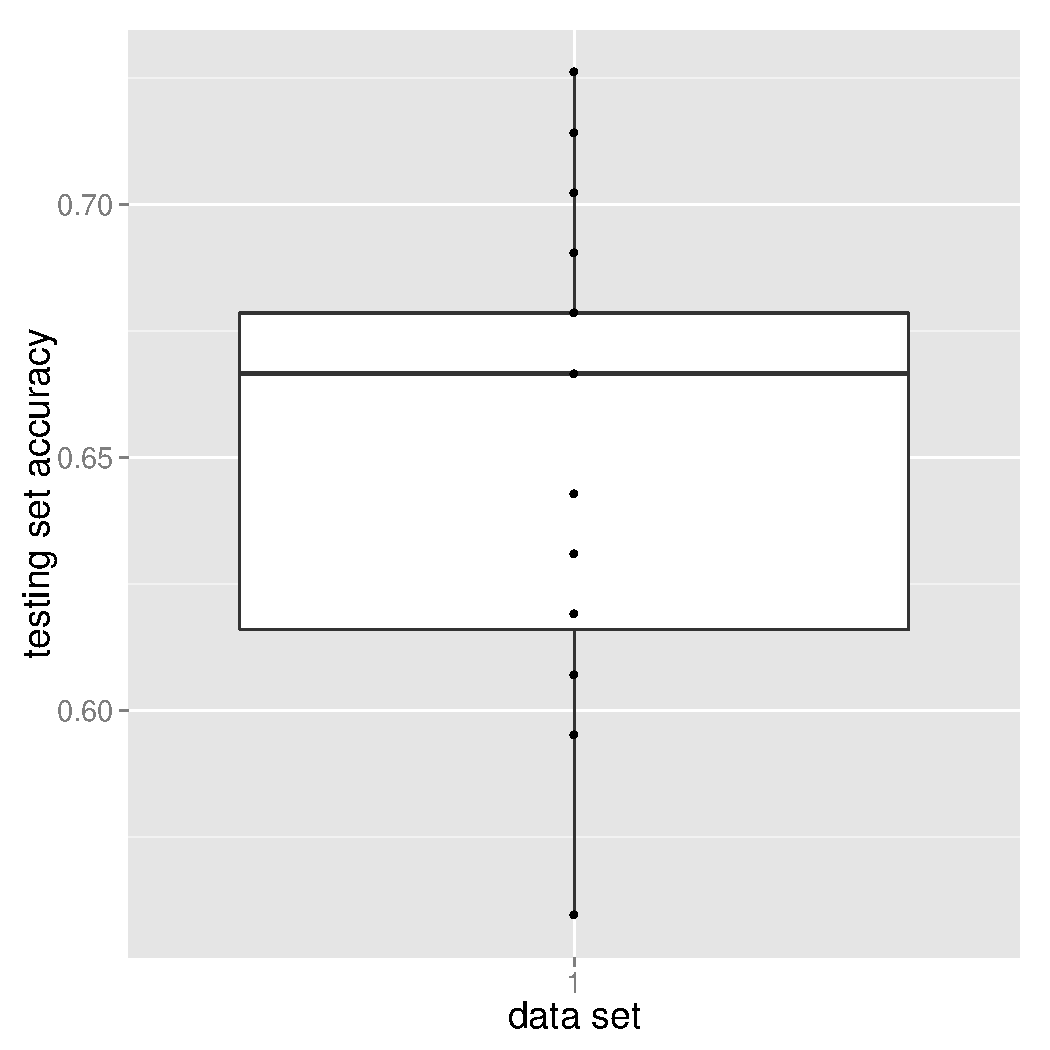
\includegraphics[width=0.34\paperwidth]{images/breast_cancer_12-svm-accuracies-learn-training_validation.pdf} & 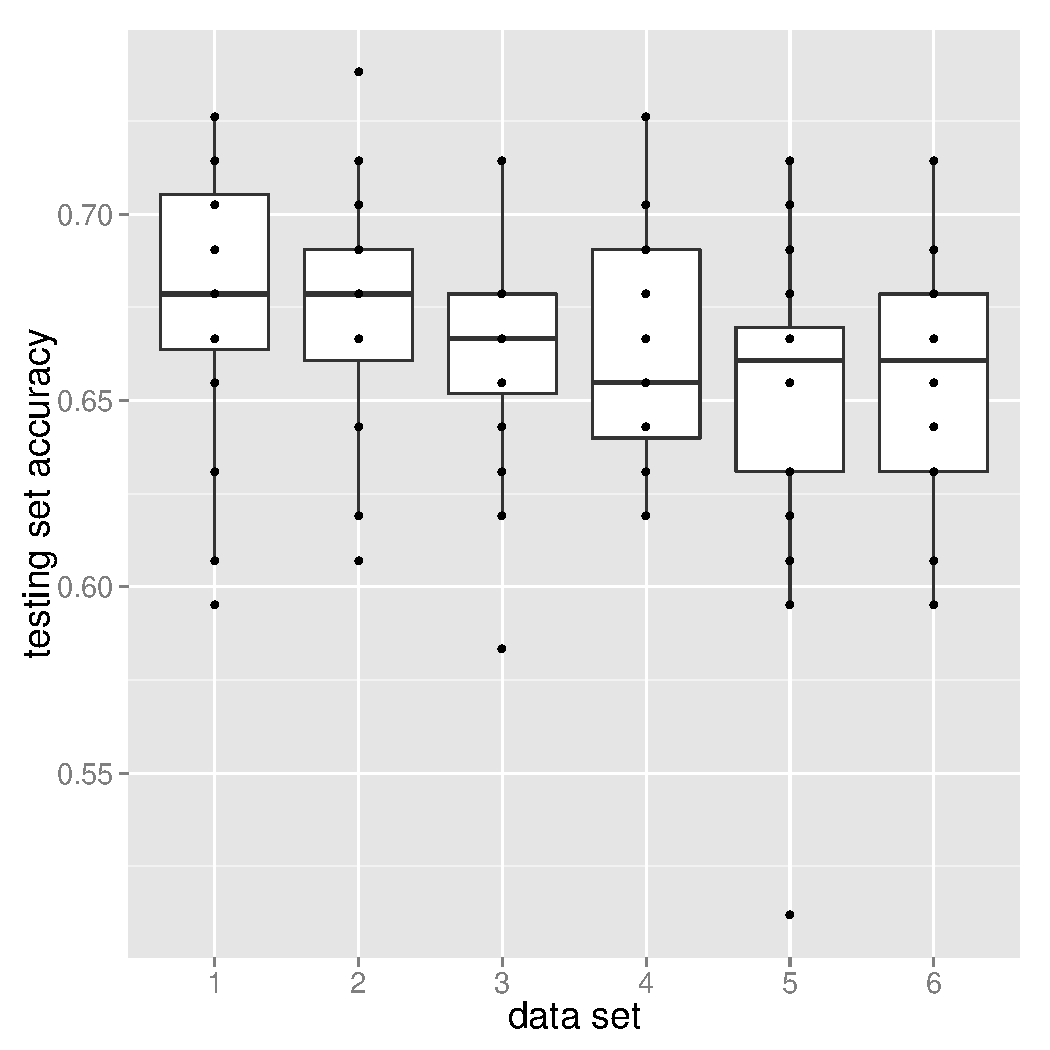
\includegraphics[width=0.34\paperwidth]{images/breast_cancer_12-svmlight-accuracies-learn_training_validation.pdf}\tabularnewline
\end{tabular}
\par\end{centering}
\caption[Accuracy comparison of supervised feed-forward network, semi-supervised
Deep Belief Network, supervised support vector machine, and semi-supervised
transductive support vector machine.]{\label{fig:Accuracy-comparison-of-breast_cancer_12}Accuracy comparison
of (a) supervised feed-forward network, (b) semi-supervised Deep Belief
Network, (c) supervised support vector machine, and (d) semi-supervised
transductive support vector machine. On the x-axis of each plot are
the sub-data-sets (of breast\_cancer\_12) predicted for each algorithm,
on the y-axis is the accuracy.}
\end{figure}

\paragraph{Paired and Two-Sided Wilcoxon Test}

Figure \ref{fig:Accuracy-comparison-of-breast_cancer_12} shows that
there is no clear improvement by increasing the number of unlabeled
samples, neither when using a DBN, nor a TSVM.

This can be quantified using a paired and two-sided Wilcoxon test\index{Wilcoxon test}.
It is paired over the repetitions because the labeled training and
validation sets are constant across data sets 1-6 within a repetition
and the only difference is the amount of unlabeled data used during
training. It is two-sided because we do not know before the experiment
which algorithm on a data set will perform better than another. The
null hypothesis is that the true accuracy shift between the two compared
experiments is zero.

By experiment we mean the set of accuracies in figure \ref{fig:Accuracy-comparison-of-breast_cancer_12}
when keeping the prediction method and sub-data-set of breast\_cancer\_12
constant, but varying the repetition. Hence there are 1 FFN, 5 DBN,
1 SVM, and 6 TSVM experiments.

We could now compare all experiments against all other experiments
using a Wilcoxon test. However, this would be ``fishing for significance'',
and we would have to correct the p-values for multiple testing. If
comparing all against all, there are $(1+5+1+6)*(1+5+1+6-1)/2=78$
comparisons, and we would lose a lot of power due to comparisons that
are not interesting. That is why we only compare the experiments in
figure \ref{fig:Accuracy-comparison-of-breast_cancer_12} row-wise
and column-wise, because these comparisons allow an interpretation.
That way there are only $1*5+1*6+1*1+5*6=42$ comparisons. We adjust
the p-values within each comparison only.

\subsubsection{Comparison of FFN With DBN}

Table \ref{tab:breast_cancer_12-FFN-versus-DBN} compares a supervised
Feed-Forward Network (FFN) against a semi-supervised Deep Belief Network
(DBN). Because the FFN is trained supervisedly, it cannot be trained
on data sets 2-6, which contain unlabeled samples.

\begin{table}[p]
\begin{centering}
\begin{tabular}{|c|c|c|c|c|c|c|c|c|}
\hline 
n1 & method1 & n2 & method2 & p\_value & estimate & ci\_lower & ci\_upper & p\_adjust\tabularnewline
\hline 
\hline 
1 & FFN & 2 & DBN & 0.896 & 0.000 & -0.007 & 0.009 & 0.955\tabularnewline
\hline 
1 & FFN & 3 & DBN & 0.255 & 0.005 & -0.004 & 0.013 & 0.637\tabularnewline
\hline 
1 & FFN & 4 & DBN & 0.723 & 0.001 & -0.009 & 0.009 & 0.955\tabularnewline
\hline 
1 & FFN & 5 & DBN & 0.255 & 0.004 & -0.003 & 0.011 & 0.637\tabularnewline
\hline 
1 & FFN & 6 & DBN & 0.955 & 0.000 & -0.010 & 0.007 & 0.955\tabularnewline
\hline 
\end{tabular}
\par\end{centering}
\caption[Comparison of FFN with DBN.]{\label{tab:breast_cancer_12-FFN-versus-DBN}Comparison of FFN with
DBN. Columns \emph{n1} and \emph{n2} are the sub-data-set indices
to be compared. (A higher index means means this sub-data-set has
more unlabeled samples than a lower index.) \emph{method1} and \emph{method2}
are the methods to be compared. \emph{p\_value} is the unadjusted
p-value, \emph{estimate} is the estimated difference in accuracy of
the comparison (e.g. 0.1 would mean method1's accuracy is better by
an estimated 10 percent points), \emph{ci\_lower} and \emph{ci\_upper}
are the lower and upper confidence interval for the estimated accuracy
difference. \emph{p\_adjust} is the p-value corrected for multiple
testing. Raw and adjusted p-values below 5\% are written in bold font.}
\end{table}

The lowest adjusted p-value is 0.637, which means there is no significant
difference between FFN and DBN.

\subsubsection{Comparison of SVM With TSVM}

Table \ref{tab:breast_cancer_12-SVM-versus-TSVM} compares a supervised
Support Vector Machine (SVM) against a semi-supervised Transductive
Support Vector Machine (TSVM). Because the SVM is trained supervisedly,
it cannot be trained on data sets 2-6, which contain unlabeled samples.

\begin{table}[p]
\begin{centering}
\begin{tabular}{|c|c|c|c|c|c|c|c|c|}
\hline 
n1 & method1 & n2 & method2 & p\_value & estimate & ci\_lower & ci\_upper & p\_adjust\tabularnewline
\hline 
\hline 
1 & SVM & 1 & TSVM & \textbf{0.026} & -0.024 & -0.054 & 0.000 & 0.158\tabularnewline
\hline 
1 & SVM & 2 & TSVM & 0.104 & -0.018 & -0.042 & 0.006 & 0.313\tabularnewline
\hline 
1 & SVM & 3 & TSVM & 0.240 & -0.012 & -0.042 & 0.012 & 0.359\tabularnewline
\hline 
1 & SVM & 4 & TSVM & 0.191 & -0.012 & -0.036 & 0.012 & 0.359\tabularnewline
\hline 
1 & SVM & 5 & TSVM & 0.779 & 0.000 & -0.030 & 0.024 & 0.779\tabularnewline
\hline 
1 & SVM & 6 & TSVM & 0.588 & -0.006 & -0.024 & 0.018 & 0.706\tabularnewline
\hline 
\end{tabular}
\par\end{centering}
\caption[Comparison of SVM with TSVM.]{\label{tab:breast_cancer_12-SVM-versus-TSVM}Comparison of SVM with
TSVM. See table \ref{tab:breast_cancer_12-FFN-versus-DBN} for the
legend.}
\end{table}

The lowest adjusted p-value is 0.158 between SVM and TSVM on data
set 1.

\subsubsection{Comparison of FFN With SVM}

Table \ref{fig:breast_cancer_12-FFN-versus-SVM} compares a non-linear
Feed-Forward Network against a Support Vector Machine with linear
kernel. Both algorithms are supervised.

\begin{table}[p]
\begin{centering}
\begin{tabular}{|c|c|c|c|c|c|c|c|c|}
\hline 
n1 & method1 & n2 & method2 & p\_value & estimate & ci\_lower & ci\_upper & p\_adjust\tabularnewline
\hline 
\hline 
1 & FFN & 1 & SVM & 0.926 & -0.003 & -0.023 & 0.021 & 0.926\tabularnewline
\hline 
\end{tabular}
\par\end{centering}
\caption[Comparison of FFN with SVM.]{\label{fig:breast_cancer_12-FFN-versus-SVM}Comparison of FFN with
SVM. See table \ref{tab:breast_cancer_12-FFN-versus-DBN} for the
legend.}
\end{table}

The p-value is 0.926 and not significant.

\subsubsection{Comparison of DBN With TSVM}

Table \ref{tab:breast_cancer_12-TSVM-versus-DBN} compares a non-linear
Deep Belief Network against a Transductive Support Vector Machine
with linear kernel. Both algorithms are semi-supervised.

\begin{table}[p]
\begin{centering}
\begin{tabular}{|c|c|c|c|c|c|c|c|c|}
\hline 
n1 & method1 & n2 & method2 & p\_value & estimate & ci\_lower & ci\_upper & p\_adjust\tabularnewline
\hline 
\hline 
1 & TSVM & 2 & DBN & \textbf{0.002} & 0.023 & 0.009 & 0.043 & \textbf{0.012}\tabularnewline
\hline 
1 & TSVM & 3 & DBN & \textbf{0.000} & 0.031 & 0.018 & 0.044 & \textbf{0.004}\tabularnewline
\hline 
1 & TSVM & 4 & DBN & \textbf{0.000} & 0.025 & 0.014 & 0.037 & \textbf{0.004}\tabularnewline
\hline 
1 & TSVM & 5 & DBN & \textbf{0.000} & 0.029 & 0.018 & 0.040 & \textbf{0.004}\tabularnewline
\hline 
1 & TSVM & 6 & DBN & \textbf{0.001} & 0.027 & 0.013 & 0.043 & \textbf{0.011}\tabularnewline
\hline 
2 & TSVM & 2 & DBN & 0.065 & 0.020 & -0.001 & 0.043 & 0.129\tabularnewline
\hline 
2 & TSVM & 3 & DBN & \textbf{0.009} & 0.023 & 0.006 & 0.039 & \textbf{0.047}\tabularnewline
\hline 
2 & TSVM & 4 & DBN & \textbf{0.016} & 0.021 & 0.005 & 0.036 & 0.060\tabularnewline
\hline 
2 & TSVM & 5 & DBN & \textbf{0.016} & 0.022 & 0.005 & 0.038 & 0.060\tabularnewline
\hline 
2 & TSVM & 6 & DBN & \textbf{0.029} & 0.022 & 0.003 & 0.040 & 0.087\tabularnewline
\hline 
3 & TSVM & 2 & DBN & 0.113 & 0.016 & -0.003 & 0.035 & 0.199\tabularnewline
\hline 
3 & TSVM & 3 & DBN & \textbf{0.050} & 0.017 & 0.000 & 0.036 & 0.115\tabularnewline
\hline 
3 & TSVM & 4 & DBN & \textbf{0.035} & 0.016 & 0.004 & 0.029 & 0.095\tabularnewline
\hline 
3 & TSVM & 5 & DBN & \textbf{0.024} & 0.017 & 0.003 & 0.031 & 0.080\tabularnewline
\hline 
3 & TSVM & 6 & DBN & \textbf{0.042} & 0.014 & 0.001 & 0.030 & 0.105\tabularnewline
\hline 
4 & TSVM & 2 & DBN & 0.211 & 0.012 & -0.009 & 0.035 & 0.333\tabularnewline
\hline 
4 & TSVM & 3 & DBN & 0.070 & 0.018 & -0.001 & 0.032 & 0.132\tabularnewline
\hline 
4 & TSVM & 4 & DBN & 0.131 & 0.013 & -0.003 & 0.026 & 0.218\tabularnewline
\hline 
4 & TSVM & 5 & DBN & 0.059 & 0.014 & -0.001 & 0.030 & 0.127\tabularnewline
\hline 
4 & TSVM & 6 & DBN & 0.225 & 0.011 & -0.006 & 0.028 & 0.338\tabularnewline
\hline 
5 & TSVM & 2 & DBN & 0.614 & 0.005 & -0.018 & 0.029 & 0.658\tabularnewline
\hline 
5 & TSVM & 3 & DBN & 0.467 & 0.007 & -0.013 & 0.025 & 0.538\tabularnewline
\hline 
5 & TSVM & 4 & DBN & 0.422 & 0.007 & -0.011 & 0.021 & 0.533\tabularnewline
\hline 
5 & TSVM & 5 & DBN & 0.444 & 0.007 & -0.011 & 0.024 & 0.533\tabularnewline
\hline 
5 & TSVM & 6 & DBN & 0.641 & 0.003 & -0.014 & 0.021 & 0.663\tabularnewline
\hline 
6 & TSVM & 2 & DBN & 0.514 & 0.006 & -0.012 & 0.025 & 0.571\tabularnewline
\hline 
6 & TSVM & 3 & DBN & 0.380 & 0.006 & -0.006 & 0.020 & 0.519\tabularnewline
\hline 
6 & TSVM & 4 & DBN & 0.444 & 0.005 & -0.011 & 0.018 & 0.533\tabularnewline
\hline 
6 & TSVM & 5 & DBN & 0.360 & 0.006 & -0.009 & 0.021 & 0.515\tabularnewline
\hline 
6 & TSVM & 6 & DBN & 0.896 & 0.001 & -0.012 & 0.017 & 0.896\tabularnewline
\hline 
\end{tabular}
\par\end{centering}
\caption[Comparison of DBN with TSVM.]{\label{tab:breast_cancer_12-TSVM-versus-DBN}Comparison of DBN with
TSVM. See table \ref{tab:breast_cancer_12-FFN-versus-DBN} for the
legend.}
\end{table}

Due to their p-values being smaller than 5\%, we can conclude that
the TSVM on data set 1 is significantly better than the DBN on all
data sets. In addition, the SVM on data set 2 is significantly better
than the DBN on data set 3. For example, the TSVM trained on sub-data-set
1 is better than the DBN trained on sub-data-set 2 by 2.3 percent
points in accuracy.

The result that the TSVM on data set 1 is better than the DBNs, and
not on data set 5 or 6, which consist of more unlabeled data, is contrary
to the expected hypothesis that a semi-supervised TSVM trained on
more unlabeled samples is better than one on less unlabeled samples.

The table also shows that the advantage of using a TSVM over a DBN
becomes negligible when adding more unlabeled data to training. (The
``estimate'' value declines with increasing data set, from 2.0\%
on data set 2 versus data set 2 to 0.1\% on data set 6 versus data
set 6.)

\subsubsection{Comparison of TSVM With TSVM}

The largest differences in prediction accuracy are within TSVM. Due
to it being semi-supervised we were interested in whether there are
significant accuracy differences within the sub-data-sets of breast\_cancer\_12.
Table \ref{tab:breast_cancer_12-TSVM-versus-TSVM} compares all TSVMs
on the sub-data-sets against all other TSVM on the sub-data-sets.

\begin{table}
\begin{centering}
\begin{tabular}{|c|c|c|c|c|c|c|c|c|}
\hline 
n1 & method1 & n2 & method2 & p\_value & estimate & ci\_lower & ci\_upper & p\_adjust\tabularnewline
\hline 
\hline 
1 & TSVM & 2 & TSVM & 0.254 & 0.012 & -0.012 & 0.030 & 0.347\tabularnewline
\hline 
1 & TSVM & 3 & TSVM & 0.184 & 0.018 & -0.006 & 0.036 & 0.320\tabularnewline
\hline 
1 & TSVM & 4 & TSVM & 0.061 & 0.018 & 0.000 & 0.036 & 0.182\tabularnewline
\hline 
1 & TSVM & 5 & TSVM & \textbf{0.023} & 0.030 & 0.006 & 0.048 & 0.113\tabularnewline
\hline 
1 & TSVM & 6 & TSVM & \textbf{0.007} & 0.030 & 0.012 & 0.048 & \textbf{0.098}\tabularnewline
\hline 
2 & TSVM & 3 & TSVM & 0.588 & 0.006 & -0.006 & 0.024 & 0.679\tabularnewline
\hline 
2 & TSVM & 4 & TSVM & 0.222 & 0.012 & -0.006 & 0.024 & 0.332\tabularnewline
\hline 
2 & TSVM & 5 & TSVM & \textbf{0.015} & 0.018 & 0.006 & 0.030 & 0.110\tabularnewline
\hline 
2 & TSVM & 6 & TSVM & \textbf{0.031} & 0.024 & 0.006 & 0.030 & 0.115\tabularnewline
\hline 
3 & TSVM & 4 & TSVM & 0.759 & 0.000 & -0.012 & 0.018 & 0.813\tabularnewline
\hline 
3 & TSVM & 5 & TSVM & 0.192 & 0.012 & -0.006 & 0.024 & 0.320\tabularnewline
\hline 
3 & TSVM & 6 & TSVM & 0.154 & 0.012 & -0.006 & 0.030 & 0.320\tabularnewline
\hline 
4 & TSVM & 5 & TSVM & 0.313 & 0.012 & -0.012 & 0.030 & 0.391\tabularnewline
\hline 
4 & TSVM & 6 & TSVM & 0.110 & 0.012 & 0.000 & 0.024 & 0.274\tabularnewline
\hline 
5 & TSVM & 6 & TSVM & 0.977 & 0.000 & -0.024 & 0.018 & 0.977\tabularnewline
\hline 
\end{tabular}
\par\end{centering}
\caption[Comparison of TSVM with TSVM on different numbers of unlabeled samples.]{\label{tab:breast_cancer_12-TSVM-versus-TSVM}Comparison of TSVM
with TSVM on different numbers of unlabeled samples. See table \ref{tab:breast_cancer_12-FFN-versus-DBN}
for the legend. Duplicate rows were removed.}
\end{table}

The lowest adjusted p-value is 0.098 between data set 1 and data set
6. Again, this is contrary to the expected hypothesis that adding
unlabeled data in the training of the semi-supervised TSVM is beneficial
to its prediction accuracy.

\section{Less Network Parameters\label{sec:breast_cancer_15}}

Since breast\_cancer\_12 has a negative result in summary, because
it cannot confirm the benefit of adding unlabeled samples to training,
in data set \index{breast_cancer_15@breast\_cancer\_15}breast\_cancer\_15
we considered the differences in data sources and artificial neural
network configurations between our and the ones in image recognition,
where DBNs are successful. We also increased the number of input genes
from the 500 most variable genes used as input genes in previous data
sets to all 22,283 available genes.

\subsection{Too Many Free Parameters}

\cite{HintonTeh2006} write that they use a 3-hidden-layer network
with about $1.7*10^{6}$ weights. They used 44000 training samples
with 28{*}28 pixels each. So altogether they have about 34.5 million
``training numbers'', and 1.7 million weights that have to be determined.
Precisely, their ratio of input numbers to number of weights is 
\begin{eqnarray*}
\frac{\mbox{input numbers}}{\mbox{weights}} & = & \frac{44000*28*28}{28*28*500+500*500+500*2000+2000*10}\approx20.8.
\end{eqnarray*}

In contrast to that we have (in data set breast\_cancer\_12, data
set 6) 238 training and validation samples, each of which has 500
expression levels, i.e. $238*500=119,000$ ``training numbers''
used totally in the input. The breast\_cancer\_12 artificial neural
networks all have an architecture of 500-1000-1000-2000-1 (500 input
nodes, 1000 hidden layer 1 nodes, 1000 hidden layer 2 nodes, 2000
hidden layer 3 nodes, and 1 output layer node). Hence, there are $500*1000+1000*1000+1000*2000+2000*1\approx3.5*10^{6}$
weights to be learnt. The ratio of $\frac{\mbox{input numbers}}{\mbox{weights}}\approx0.034\ll20.8$
is much lower in our case than in the image recognition case. 

This can be changed by using all $i=22,283$ genes as inputs, and
only a very small number of hidden nodes $h$ (assuming for simplicity
that all hidden layers have the same number of nodes). If we take
$i=22,283$, and there are 238 training samples (in fact we have only
20 labeled plus 100 unlabeled training samples in breast\_cancer\_12),
then we have $22,283*238=5,303,354$ measured numbers. The ratio formula
is
\begin{eqnarray*}
r(h) & = & \frac{22283*238}{22283*h+h*h+h*h+h*o},
\end{eqnarray*}
where $h$ is the number of hidden nodes and $o$ is the number of
output samples and is equal to 1, because the labeled cases have a
binary label.

\subsection{Data Set Design\label{subsec:Data-Set-Design-of-breast_cancer_15}}

To exclude that a batch effect between GSE25055 and GSE25065 negatively
affects semi-supervised learning, in breast\_cancer\_15 we only use
GSE25055, also for testing. Again we use 10\textbar{}10 labeled training
and validation samples. This leaves us with remaining $57-20=37$
label 1 samples for testing, and we also use 37 label 0 samples. Like
in previous data sets, all samples for the labeled training and validation
data sets can be re-used in the unlabeled data set, because the labels
are not given to the neural network during pre-training.

We choose a reasonably large unlabeled validation data set of 28 samples
like in breast\_cancer\_12 (although in breast\_cancer\_12 we used
21 GSE25065 samples in addition). The ratio of label 0 to label 1
samples is $249/57\approx4.37$. To have a sufficient number of label
1 unlabeled validation samples, we use $100|25$ (where $x|y$ means
$x$ label 0 samples and $y$ label 1 samples) unlabeled validation
samples, where the 25 label 1 samples are replicated 4 times (written
$100|25*4$). This leaves $57-25=32$ label 1 samples for the unlabeled
training data set. Replicating label 1 samples 4 times in the data
set to have the same ratio of different label 0 and label 1 samples
as in the unlabeled validation data set gives $128|32*4=128|128$
samples.

Altogether, there are in the labeled and unlabeled training data $10|10+128|32*4=138|138$
samples = 276 samples, when counting the quadrupled label 1 samples
as 4 individual samples. When counting the quadrupled samples as only
1 real sample, there are $10|10+128|32=10*2+128+32=180$ samples.
So $t_{quad}=276$, $t_{indiv}=180$, $o=1$.

The ratio is then 
\begin{eqnarray*}
r(h,t) & = & \frac{22283*t}{22283*h+h*h+h*h+h*o}.
\end{eqnarray*}
For a hidden layer size of $h=10$, $r(h,t)$ is shown in table \ref{tab:breast_cancer_12-number-r}
for the 6 different data sets (containing an increasing number of
samples $t$).
\begin{table}
\begin{centering}
\begin{tabular}{|c||c|c|c|c|c|c|}
\hline 
data set & 1 & 2 & 3 & 4 & 5 & 6\tabularnewline
\hline 
\hline 
$t_{quad}$ & 2{*}10 & 2{*}(10+24) & 2{*}(10+52) & 2{*}(10+76) & 2{*}(10+104) & 2{*}(10+128)\tabularnewline
\hline 
$r(10,t_{quad})$ & 2.00 & 6.79 & 12.39 & 17.18 & 22.78 & 27.57\tabularnewline
\hline 
$t_{indiv}$ & 2{*}10 & 20+24+6 & 20+52+13 & 20+76+19 & 20+104+26 & 20+128+32\tabularnewline
\hline 
$r(10,t_{indiv})$ & 2.00 & 5.00 & 8.49 & 11.49 & 14.99 & 17.98\tabularnewline
\hline 
\end{tabular}
\par\end{centering}
\caption[The ratio of training samples to network parameters for 10 hidden
nodes.]{\label{tab:breast_cancer_12-number-r}The ratio of training samples
to network parameters, $r$,  for 10 hidden nodes in data set breast\_cancer\_15.
$t_{quad}$ is the number of samples when counting quadrupled samples
as 4 samples. $t_{indiv}$ is the number of samples when quadrupled
samples are counted as 1 sample.}
\end{table}
As the values for $r$ in the table are around 20 (for data set 6),
both for $t_{quad}$ and $t_{indiv}$, we choose a hidden layer node
size $h=10$. The architecture for the artificial neural networks
of breast\_cancer\_15 is 22283-10-10-10-1.

Another big change compared to previous data sets is the use of all
22,283 genes as input instead of only the 500 most variable genes.

The complete data set is shown in table \ref{tab:design-of-breast_cancer_15}.

\begin{table}
\begin{centering}
\begin{tabular}{|c|c|c||c|c|c|c|c|c|}
\hline 
\multicolumn{3}{|c||}{data set} & 1 & 2 & 3 & 4 & 5 & 6\tabularnewline
\hline 
\hline 
\multirow{6}{*}{\begin{turn}{90}
labeled
\end{turn}} & \multirow{2}{*}{testing} & GSE25055 & \multicolumn{6}{c|}{37\textbar{}37}\tabularnewline
\cline{3-9} 
 &  & GSE25065 & \multicolumn{6}{c|}{0\textbar{}0}\tabularnewline
\cline{2-9} 
 & \multirow{2}{*}{training} & GSE25055 & \multicolumn{6}{c|}{10\textbar{}10}\tabularnewline
\cline{3-9} 
 &  & GSE25065 & \multicolumn{6}{c|}{0\textbar{}0}\tabularnewline
\cline{2-9} 
 & \multirow{2}{*}{validation} & GSE25055 & \multicolumn{6}{c|}{10\textbar{}10}\tabularnewline
\cline{3-9} 
 &  & GSE25065 & \multicolumn{6}{c|}{0\textbar{}0}\tabularnewline
\hline 
\multirow{6}{*}{\begin{turn}{90}
unlabeled
\end{turn}} & \multirow{3}{*}{training} & GSE25055 & 0\textbar{}0 & 24\textbar{}6{*}4 & 52\textbar{}13{*}4 & 76\textbar{}19{*}4 & 104\textbar{}26{*}4 & 128\textbar{}32{*}4\tabularnewline
\cline{3-9} 
 &  & GSE25065 & \multicolumn{6}{c|}{0\textbar{}0}\tabularnewline
\cline{3-9} 
 &  & $\sum_{Training}$ & 0\textbar{}0 & 24\textbar{}6{*}4 & 52\textbar{}13{*}4 & 76\textbar{}19{*}4 & 104\textbar{}26{*}4 & 128\textbar{}32{*}4\tabularnewline
\cline{2-9} 
 & \multirow{3}{*}{validation} & GSE25055 & 0\textbar{}0 & 20\textbar{}5{*}4 & 40\textbar{}10{*}4 & 60\textbar{}15{*}4 & 80\textbar{}20{*}4 & 100\textbar{}25{*}4\tabularnewline
\cline{3-9} 
 &  & GSE25065 & \multicolumn{6}{c|}{0\textbar{}0}\tabularnewline
\cline{3-9} 
 &  & $\sum_{Validation}$ & 0\textbar{}0 & 20\textbar{}5{*}4 & 40\textbar{}10{*}4 & 60\textbar{}15{*}4 & 80\textbar{}20{*}4 & 100\textbar{}25{*}4\tabularnewline
\hline 
\multicolumn{3}{|c||}{repeats} & 20 & 20 & 20 & 20 & 20 & 20\tabularnewline
\hline 
\end{tabular}
\par\end{centering}
\caption[Data set design of breast\_cancer\_15.]{\label{tab:design-of-breast_cancer_15}Data set design of breast\_cancer\_15.
It contains 37\textbar{}37 labeled testing, 10\textbar{}10 labeled
training, 10\textbar{}10 labeled validation, $128|32*4$ unlabeled
training, and $100|25*4$ unlabeled validation samples (where $x|y*f$
means $x$ label 0 samples, and $y$ label 1 samples duplicated $f$
times). 6 sub-data-sets are created, with the first one having no
unlabeled data at all, the last one having $128|32*4$ training and
$100|25*4$ validation samples, and interpolated numbers in-between.
The labeled data are equal across all data sets (but different between
different repetitions). There are 20 sub-sampling repeats per sub-data-set.
All samples are from GSE25055, to avoid a possible batch-effect.}
\end{table}

\subsubsection{Different Training Parameters}

In comparison to breast\_cancer\_12, the unsupervised learning rate
(\emph{base\_epsilon}) was decreased from 0.01 to 0.001 for the pre-training
of hidden layer 1, and from 0.001 to 0.0001 for pre-training hidden
layers 2 and 3. We also changed the mini-batch\footnote{In training, the network parameters' deltas are alternatingly computed,
then the parameters are updated. (See equation \ref{eq:backpropagation-deltas}
in backpropagation training.) The mini-batch is the number of samples
whose deltas are accumulated before the network parameters are updated.} size from 100 to 1000, which leads to slower training, but iterates
over all training samples before changing weights, and thus approximates
the derivative of the weights more faithfully.

\subsection{Accuracy of DBN Fine-tuned with Back-propagation}

\begin{figure}
\begin{centering}
\includegraphics[width=0.68\columnwidth]{images/breast_cancer_15-accuracies-testing-aa_dv.pdf}
\par\end{centering}
\caption[Test set accuracies for different data sets with more and more unlabeled
training samples in a DBN on breast\_cancer\_15.]{\label{fig:Accuracy-in-breast_cancer_15}Box plots of test set accuracies
for different data sets with more and more unlabeled training samples
in a neural network pre-trained with DBN on breast\_cancer\_15. The
x-axis is the data sets in the order of rising number of unlabeled
samples; the y-axis is the test set accuracy. Data set 1 cannot be
used in DBNs because it does not contain unlabeled data. The y-axis
is the accuracy. Each dot represents the accuracy on a repetition.}
\end{figure}

Figure \ref{fig:Accuracy-in-breast_cancer_15} shows the accuracies
obtained for data set breast\_cancer\_15. The accuracies are better
than those obtained in breast\_cancer\_12: The median accuracy is
near 0.7 for all data sets except data set 3, while it was slightly
above 0.65 in breast\_cancer\_12. This may be due to less overfitting
because there are less model parameters, but it may also be due to
the training having used more input data (22,283 genes instead of
the 500 most significant).

To check whether there is a dependence of accuracies on the amount
of unlabeled samples available to training, we use a paired (over
the repetitions) and two-sided Wilcoxon test. The p-value for the
accuracy difference between data sets 2 and 6 is 0.089. The estimated
difference between accuracies of data sets 2 and 6 is 2.8 percent
points (0.028). (The 95\% confidence interval for the difference is
{[}-0.46; 6.7{]} percent points.) This shows a slight dependence of
accuracy on the number of unlabeled samples.

\subsection{TSVM Accuracies}

A TSVM was trained on the training and validation data of each repetition
of all data sets in breast\_cancer\_15. Figure \ref{fig:Accuracy-box-plots-of-breast_cancer_15}
shows the accuracies on the test sets. Inexplicably, training failed
in data set 2. Except for data set 2, one can see a slight accuracy
increase from data set 1 to data set 6, i.e. from the data set with
no unlabeled samples to the data set with the most unlabeled samples.
The accuracy difference between data sets 1 and 6 was tested for significance
with a paired (over the repetitions) and two-sided Wilcoxon test.
It is significant with a p-value of 0.0029, and the accuracy difference
between data sets 1 and 6 is an estimated 3.38 percent points (0.0338),
while its 95\% confidence interval is {[}2.02; 6.08{]} percent points.
Thus, in breast\_cancer\_15, the TSVM succeeded in increasing accuracy
slightly by learning from unlabeled samples.

When training a TSVM only on the training data (but leaving away the
validation data), in addition to data set 2, also data set 3 fails
to train a proper model with almost all their accuracies at 0.5, and
data set 4 has a median accuracy of only $\approx$0.575 (data not
shown). This may show that semi-supervised training using a TSVM fails
when not a sufficient number of unlabeled training samples is available.
Training the TSVM (supervisedly) using data set 1 did not fail.

\begin{figure}
\begin{centering}
\includegraphics[width=0.68\columnwidth]{images/breast_cancer_15-accuracies-svmlight.pdf}
\par\end{centering}
\caption[TSVM accuracies box plots on data set breast\_cancer\_15.]{\label{fig:Accuracy-box-plots-of-breast_cancer_15}TSVM accuracies
box plots on data set breast\_cancer\_15. On the x-axis are the data
sets in order of increasing number of unlabeled samples. On the y-axis
are the accuracies. Each dot is the accuracy of a repetition of a
data set of breast\_cancer\_15.}
\end{figure}



\cleardoublepage{}

\part{Discussion}


\section{Discussion}

We evaluated whether adding unlabeled data to semi-supervised training
is beneficial in deep neural networks, when predicting breast cancer
recurrence after chemotherapy.

\subsection{Related Work}

\paragraph{Using Tumour Expression Data Directly to Classify Recurrence}

We predicted breast cancer recurrence after reductive surgery with
neoadjuvant chemotherapy directly from expression data. Papers that
use neural networks to classify cancerous tissue are for example \cite{ChenHuang2002}
and \cite{ErcalMoss1994}. In \cite{SharafTsokos2015}, Sharaf and
Tsokos predict from 4 input variables the survival time by training
a neural network on 69,000 patients.

We selected the GSE25055 and GSE25065 data sets because they are among
the largest labeled cancer data sets in GEO that come from a single
source. Like in \cite{HatzisSymmans2011}, the larger data set GSE25055
was used for training a classifier, and the data set of independent
cases GSE25065 was used to test the classifier. We used artificial
neural networks as classifiers by predicting the class 1 probability
of the samples.

\paragraph{Neural Networks are Attractive}

In our view, neural networks have attractive properties: they are
non-linear, they can be used generatively, their implementations are
often modular (e.g. regularizations and network parameters), and in
prediction deep neural networks often are among the best predictors
in several machine learning fields. As \cite{BiganzoliMarubini1998}
 put it: ``Feed forward ANNs are strictly equivalent to non-linear
multivariate regression methods.'' They can be used unsupervisedly
as well as supervisedly. For example, to obtain a probability for
a class like done in \cite{AppelSpang2011} is straightforward, because
the network outputs class probabilities anyways. Last, but not least,
artificial neural networks are plausible models of the real biological
neural networks, which are the control centers of animals, and were
shaped by evolution during millions of years. However, neural networks'
versatility can also be a disadvantage: it is often not clear what
component or parameter to modify to achieve a desired result.

\paragraph{Differences Between Object Recognition Tasks and Cancer Recurrence
Prediction}

In different settings the pre-training and back-propagation approach
worked well \cite{ErhanBengio2010}. There are some differences between
those fields and the scenario of microarray expression data: The dimensionality
of microarrays is usually higher than that of images or phonemes (\textasciitilde{}1000
pixels versus \textasciitilde{}20,000 genes), but the training set
sizes are several magnitudes smaller (thousands to tenthousands images
versus tens to hundreds microarray data sets). For example, in the
image classification task in the ImageNet Large Scale Visual Recognition
Challenge \cite{RussakovskyFeiFei2015}, there are an average of $\approx$1,200
images per class, while in the GSE25055 data set, there are 249 class
0 and 57 class 1 samples.

The fact that there is a much smaller number of labeled and unlabeled
samples in expression data than in image recognition is probably due
to several factors: price, logistical and ethical issues. The price
of microarrays (and RNASeq) is magnitudes larger (hundreds of Euros
or dollars) than the price to take and label pictures of hand-written
digits or objects (images are ubiquitous on the internet, and manual
or computer-assisted labeling is relatively cheap). In addition, expression
data aquisition does not merely consist of putting cDNA onto microarrays,
but the process also involves selecting patients according to ethical
criteria, keeping track of patients' whereabouts and collecting clinical
parameters over an extended time-span (``follow-up'').

The difficulty of the learning task seems higher than that of recognizing
digits, where accuracies of 96\% can be achieved by nearest neighbor
classifiers. However, it may be comparable to the object recognition
tasks, that had accuracies around 70\% using SVMs in the ImageNet
Large Scale Visual Recognition Challenge.

\subsection{Summary of Own Approaches}

To sum up, we tried different training parameters, different network
architectures (with many free parameters relative to training data
set size, and with few free parameters), different normalizations,
different data set compositions. A small improvement in testing set
accuracy was achieved by using additional unlabeled data during training.

\paragraph{Different Network Configurations}

As pre-training algorithms we assessed autoencoders, Restricted Boltzmann
Machines, and Deep Belief Networks. There seemed to be only little
difference in test set accuracy between these pre-training algorithms.
However, some authors have reported that autoencoders are harder to
train. In general, reconstruction error during pre-training converged
well for our cases. Sometimes one has to wait a few iterations for
the network to travel through configurations that do not seem to change
the resulting reconstruction error.

\paragraph{Different Normalizations}

We tried using different normalizations of the raw expression data:
RMA and MAS5 normalization, logarithmizing, COMBAT batch effect correction,
and ZCA whitening. We observed the effect of normalization on reconstruction
error during pre-training as well as on classification accuracy. The
reconstruction error plots seem to depend on the normalization used.
MAS5 normalized data seem to have lower reconstruction error than
RMA normalized data. The effect of different normalizations on classification
accuracy were the other way around: Of all normalizations tested,
RMA with no additional pre-processing yielded the best accuracies
in all data sets tested. Of note is that a low reconstruction error
rate does not imply a good accuracy on the test set: Although the
neuronal nets using MAS5 normalized data had a lower reconstruction
error than their RMA counterparts, MAS5 yielded a lower accuracy than
RMA.

\paragraph{Deep Networks}

We also tried deeper networks with more than one hidden layer. Using
these did not always improve accuracy. However, using more than a
few hidden layers was not systematically investigated due to limits
in computation time.

\paragraph{Model Selection}

We always selected the iteration/model of the neural network that
had the highest validation set accuracy. Few samples lead to few different
possible accuracy values. To be able to choose the best model among
candidates that have only few possible accuracies, we smoothed the
accuracies over time (or iterations), because the network's state
of parameters at a specific iteration is closest to its state of parameters
at the closest iterations. In other words, the artificial neural networks
change only little every iteration, and we want to select a model
from a stable learning period.

\paragraph{Compared Methods: Neural Networks, SVM and TSVM}

We compared Support Vector Machine (SVM) and Transductive Support
Vector Machine (TSVM) to the artificial neural networks. TSVM is a
semi-supervised version of the normal supervised SVM, and the artificial
neural networks were used with (semi-supervised) and without (supervised)
pre-training. We compared the semi-supervised and the supervised versions
of both neuronal network and Support Vector Machine.

\paragraph{Does Semi-supervised Learning Lead to Better Neural Network Classifiers?}

We used an increasing number of unlabeled samples during pre-training
to find out whether this has an effect on the accuracy achieved during
fine-tuning. In terms of \cite{Zhu2005}, we are learning an efficient
coding of the domain from unlabeled data and then perform supervised
learning on the coded samples (see their chapter 8). The approach
is similar to that of \cite{ChenXie2015}, where they used the representation
of a sample at the deepest hidden layer to do regression on (whereas
we classify the sample, using a supervised algorithm). Like \cite{Zhu2005},
we also noticed that during data set creation for semi-supervised
learning, one has to constrain the class proportions \textendash{}
in our case to 50\% for class 0 and 50\% for class 1, otherwise the
semi-supervised training often fails with predictions biased in favor
of the larger class.

Only the very last approaches tried (data set breast\_cancer\_15,
section \ref{sec:breast_cancer_15}) showed a (small) significant
benefit between those networks trained using more unlabeled samples
over those trained using less unlabeled samples. There are three differences
between these approaches and the ones before: First, we used less
hidden layer neurons. Second, we used all 22,283 genes as input instead
of only the 500 most variable genes. Third, we tested on GSE25055
instead of GSE25065. The benefit using unlabeled samples is not due
to less hidden layer neurons, since TSVM was not influenced by this
point, but also showed the benefit. Whether the benefit is due to
using all 22,283 genes or testing on the same data set as used for
training remains to be seen.

\subsection{Outlook}

\paragraph{More Advanced Prediction Schemes}

More sophisticated prediction schemes can be imagined so that the
prediction made produces more than one number: For example, in addition
to the severity of the disease after therapy (a number between 0 and
1), the number of (visibly large) metastases (a natural number) could
be trained and predicted. Such a prediction is not made in this work,
because only little clinical data was recorded in GSE25055 and GSE25065.
However, in the neural network it would be straightforward to predict
such two numbers by adding an additional (properly scaled) number
to the output layer in the training set.

\paragraph{Multiplying of Training Samples}

In most applications of deep learning there is some algorithm involved
to multiply the number of available training data sets. For example,
in image classification the training images are usually translated
by pixel or subpixel shifts, or small non-linear deformations are
applied using a warped mesh. This has the effect that a local feature
of an input training image (for example, a red pixel on green background)
is present in different input pixels in the transformed training images.
This allows producing a large number of similar training images from
an input training set. The neural network is thereby forced to learn
the property of a feature regardless of its position in the image.
Nevertheless the position of the feature will probably vary in ``real''
(not modified) images as well.

Having such a transformation for expression data would be very useful,
not only for classification using neural networks, but also other
machine learning algorithms. However, it is not at all clear what
a pre-processing equivalent to the local image deformations could
look like for mRNA abundance. Straightforward application of the image
deformation scheme would provide the neural network with input for
a gene in the dimension of a maybe completely unrelated gene. (Note
that adding some sort of noise onto the expression levels would be
equivalent to adding noise to the image, which is not equivalent to
shifting the image.)

One approach could be to use different normalization methods, parameters,
and random number seeds used in some normalization methods to obtain
multiple copies of the same raw data set, but with small changes providing
different ``points of view'' of the data.

Another possible approach could be to look for gene modules that consist
of redundant genes, and permute their expression values among the
redundacy group. This would require knowledge about gene modules in
advance.

A third approach could be to increase the number of input samples
by creating additional samples by composing them of random subsets
of other input samples. For example, take gene 1-1000 from sample
1, gene 1001-2001 from samples 2, and so on. Or maybe even better
use gene modules as learned by an RBM (see the \emph{hub features
}in Figure S3 of \cite{ChenXie2015}). There seem to be hub networks,
that have outgoing connections to many output layer genes, with many
of the hub networks having either positive outgoing weights (i.e.
that positively affect the expression of a target gene) or negative
outgoing weights, but not both.

The algorithm would work like this: Determine for each \emph{measured}
input sample the gene hub activation (by unsupervisedly training an
RBM or DBN on all input samples). This results in a vector of numbers,
one vector for each input sample; each number stands for one gene
hub activation. Permute the gene hub activations between the learned
representations, but only use representations from samples that have
the same class label. Due to the number of permutations this creates
a large number of labeled training samples (each training sample is
labeled like the measured samples used in the training sample generation).
Use these generated training samples as input for a supervised DBN.




\cleardoublepage{}

\addcontentsline{toc}{section}{List of Figures}\listoffigures

\cleardoublepage{}

\addcontentsline{toc}{section}{List of Tables}

\listoftables

\cleardoublepage{}

\addcontentsline{toc}{section}{List of Algorithms}

\listof{algorithm}{List of Algorithms}

\cleardoublepage{}

%% strangely, this cannot be in the LaTeX Preamble
\renewcommand{\refname}{Bibliography}

\bibliographystyle{myabbrvnat}
\addcontentsline{toc}{section}{\refname}\nocite{*}
\bibliography{dissertation}

\cleardoublepage{}

\addcontentsline{toc}{section}{Index}

\printindex{}
\end{document}
